% !TeX root = ../main.tex

\chapter{Methodology}
This chapter explains the methodology used to build and evaluate the Coarse-to-Fine Semantic Conflict Detection System. It describes how Philippine legal texts are collected and cleaned, and how the two-stage Retrieve-then-Entail architecture is organized. The chapter also details the creation of the ground truth dataset and the selection of candidate models. Finally, it outlines the evaluation metrics and hardware constraints, which are chosen to match the computing capacity of an average Local Government Unit (LGU).


\section{Conceptual Framework}
This section maps how data flows through the proposed system. The architecture follows an Input-Process-Output (IPO) design organized into a two-stage ``Coarse-to-Fine'' retrieve-then-entail pipeline (Figure~\ref{fig:conceptualframework}). By decoupling broad statutory candidate retrieval from compute-intensive textual entailment classification, the framework overcomes the combinatorial explosion and hardware bottlenecks that traditionally impede local legal NLP deployment. The workflow is divided into two operational phases: Phase~1 (Offline Foundation and Optimization) and Phase~2 (Live Online Retrieve-then-Entail Pipeline).

    \begin{figure}[htbp]
        \centering
        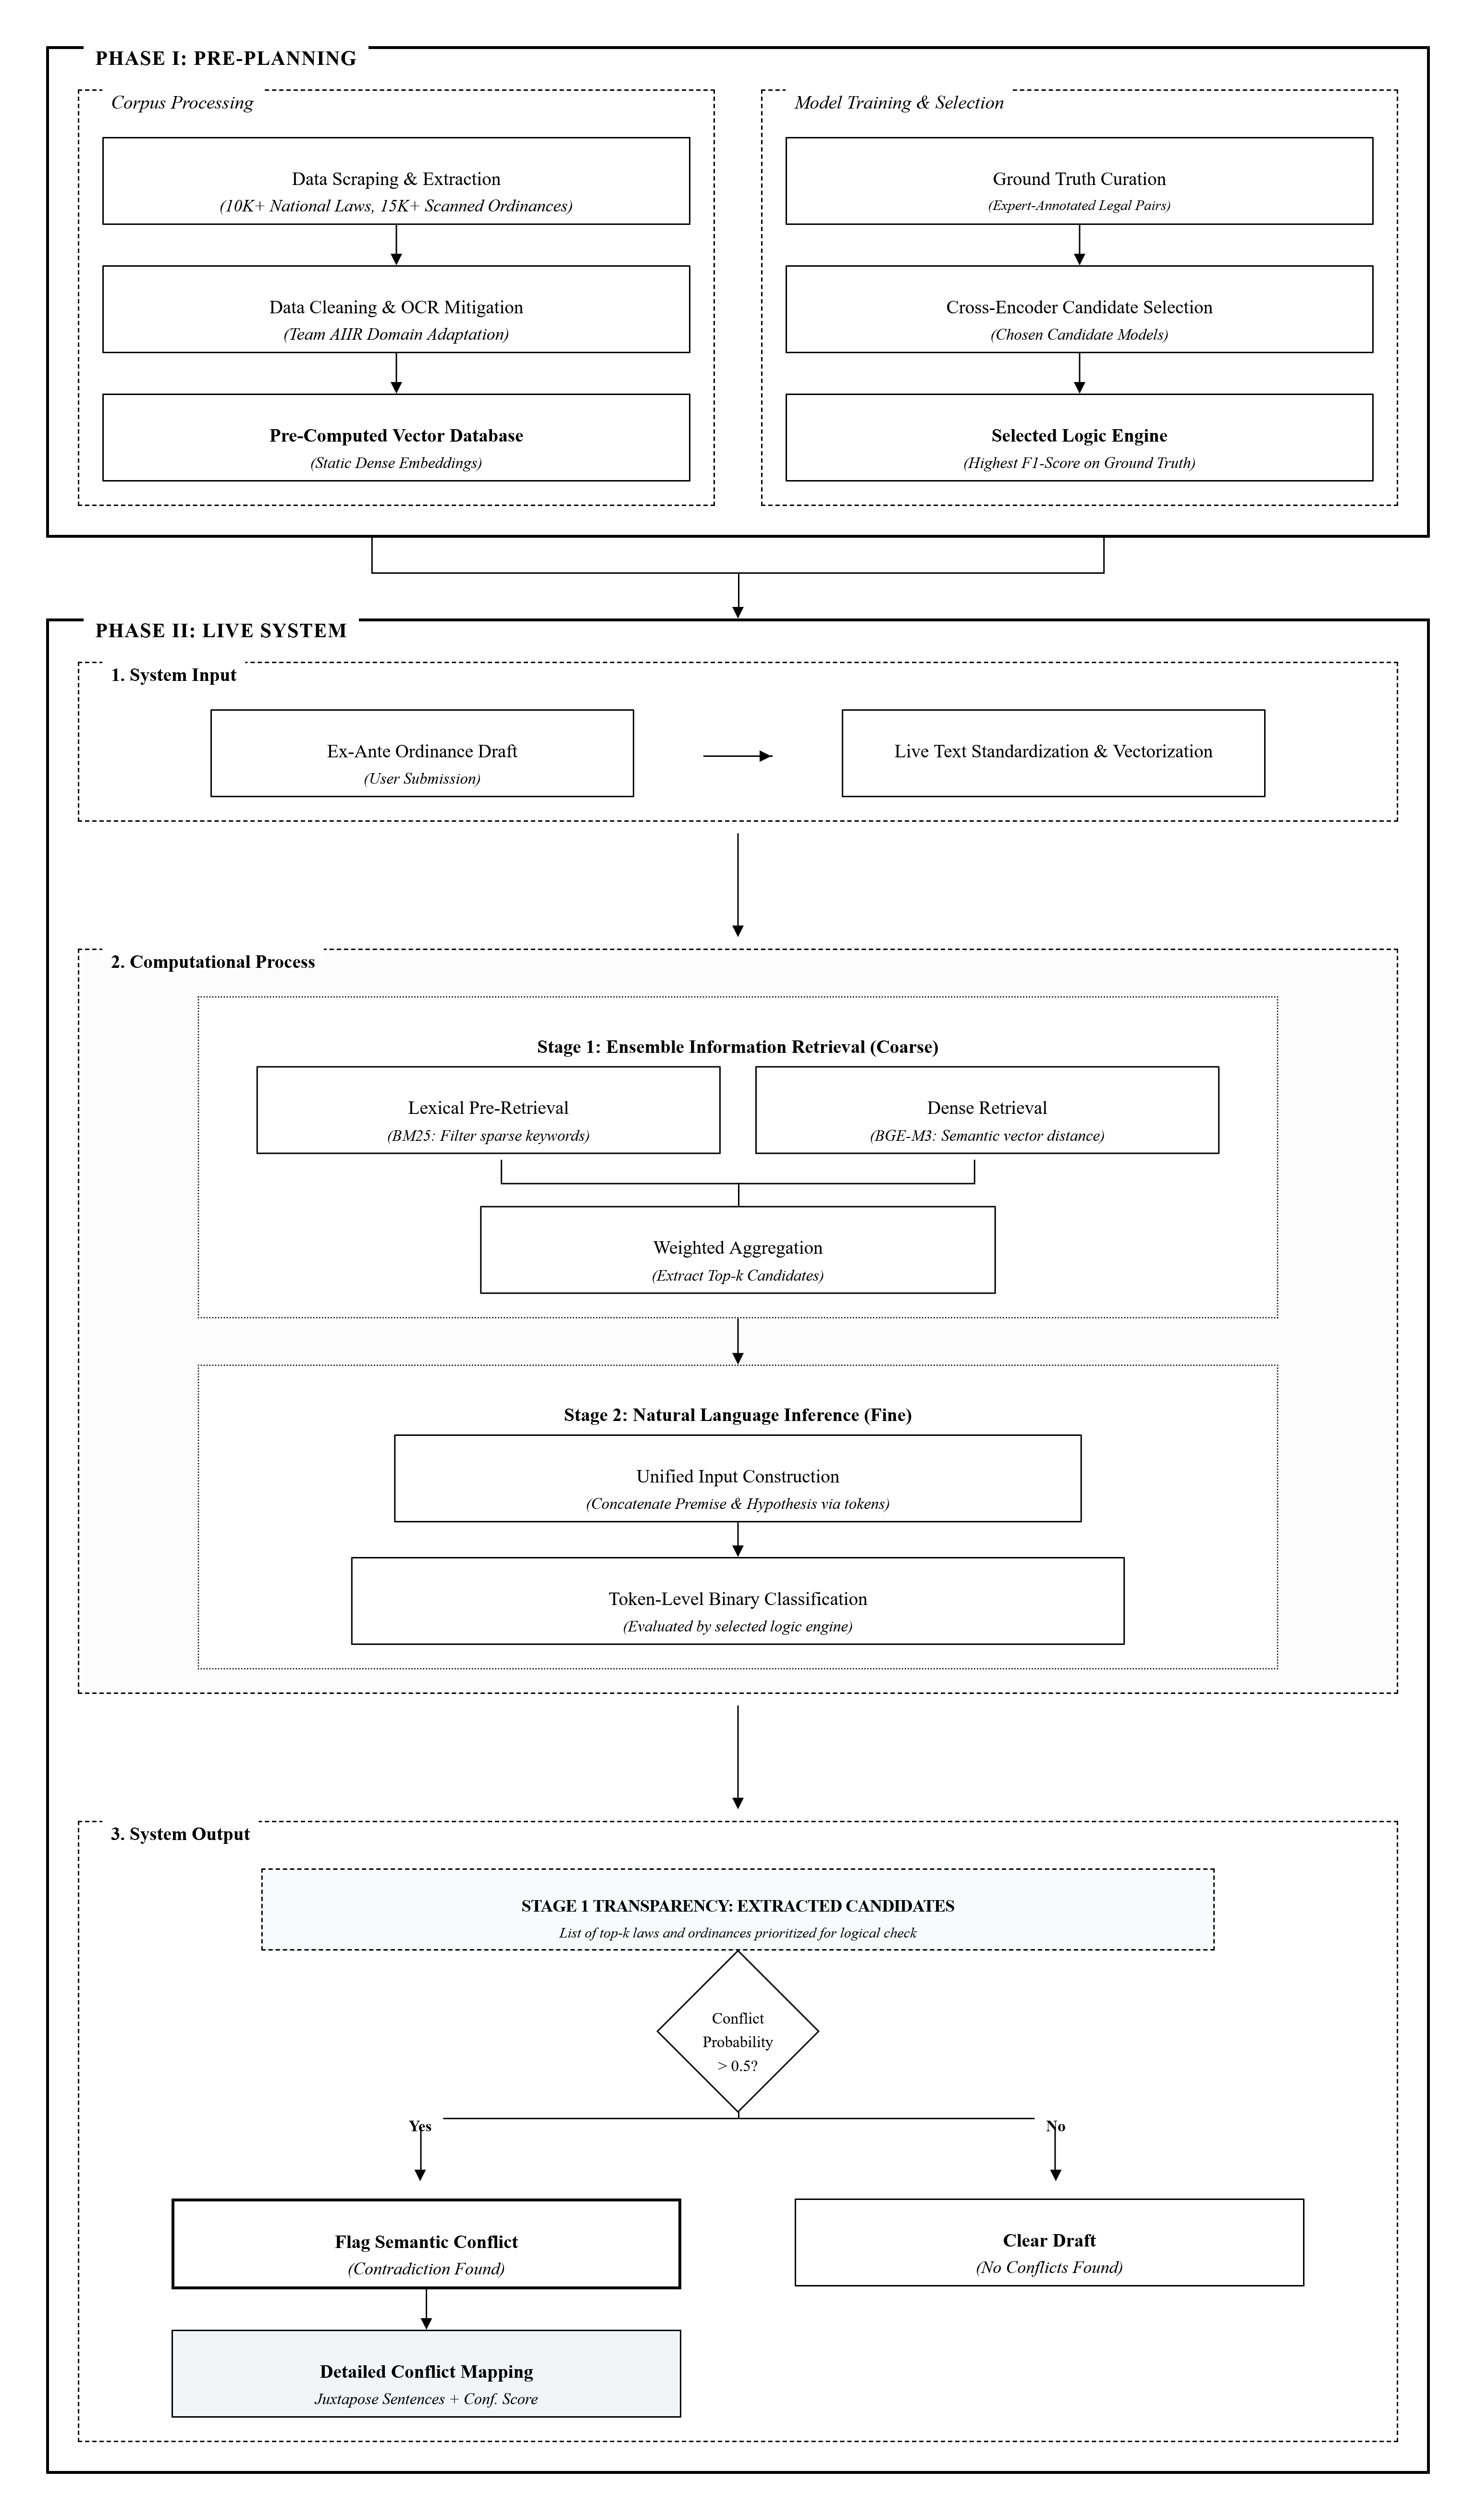
\includegraphics[width=0.88\linewidth]{figs/conceptual_framework_flowchart.png}
        \caption{Detailed Information Flow of the Coarse-to-Fine Semantic Conflict Detection Architecture.}
        \label{fig:conceptualframework}
    \end{figure}

    \subsection{Phase 1: Pre-Planning (Offline Foundation \& Optimization Protocol)}
    This preliminary phase establishes the empirical foundation of the system by compiling the statutory corpus, building pre-computed retrieval indexes, and selecting the optimal transformer logic engines through a structured benchmark screening protocol.

    \begin{description}
        \item[Dual-Corpus Ingestion \& Pre-Computation Protocol.] The system compiles a comprehensive dual-jurisdiction statutory archive combining the Philippine national statutory collection (Republic Acts, Executive Orders, Presidential Decrees, Acts, Batas Pambansa, and Commonwealth Acts) with Davao City municipal legislation (historical Landmark Ordinances and digital LISSP municipal records). The compiled corpus undergoes legal text normalization, optical character recognition (OCR) noise mitigation on historical scans, and structural section segmentation into granular, self-contained regulatory units ($\sim 200\text{--}300$ tokens). Cleaned statutory provisions are then indexed offline: dense semantic representations are pre-computed using a lightweight transformer bi-encoder, while sparse inverted lexical indexes are constructed using BM25 ($k_1 = 1.5, b = 0.75$) alongside unsupervised statutory topic modeling.
        
        \item[Model Benchmark \& Selection Protocol.] Candidate architectures are screened and fine-tuned against a curated Ground Truth Legal Benchmark stratified across three granular difficulty tiers: Tier~1 (Surface Lexical), Tier~2 (Structural Preemption), and Tier~3 (Latent Semantic). A multi-stage empirical screening and ablation protocol evaluates candidate bi-encoders (balancing inference latency against candidate Recall@$k$) and candidate cross-encoders (evaluating precision, latency, and quantization trade-offs across FP32, FP16, and INT8 axes). Based on these empirical evaluations, the highest-performing models are selected as the production engines: an optimal dense bi-encoder for Stage~1 candidate retrieval, and an optimal fine-tuned cross-encoder for Stage~2 contradiction reasoning.
    \end{description}

    \subsection{Phase 2: Live System (Online Retrieve-then-Entail Pipeline)}
    The live system executes the automated conflict detection pipeline when a newly drafted municipal measure is submitted for pre-enactment review, operating through an Input-Process-Output structure.

    \begin{description}
        \item[1. System Input.] A legislative researcher uploads a newly proposed ex-ante ordinance draft. Because draft measures originate within local government offices as digital-born documents (.docx or digital PDF), they are free from optical scanning noise. The ingestion pipeline segments the draft into individual substantive provisions, filtering out non-regulatory procedural boilerplate (such as the Title, Separability, Repealing, and Effectivity clauses). The isolated substantive provisions are vectorized in real time via the selected dense bi-encoder alongside sparse lexical token extraction.
        
        \item[2. Computational Process.] The computational core executes two complementary stages:
            \begin{description}
                \item[Stage 1: Dual-Stream Hybrid Information Retrieval.] The system narrows the comprehensive statutory search space down to a focused candidate pool. Stream~A executes lexical sparse search via BM25 to match exact statutory citations, numerical penalty amounts, and administrative agency terms. Stream~B executes dense semantic search via the selected bi-encoder, measuring cosine similarity between the draft provision and statutory embeddings to capture abstract regulatory intent. The ranked outputs are combined using Reciprocal Rank Fusion (RRF) integrated with a Statutory Hierarchy Safeguard (prioritizing higher-ranking national statutes over municipal provisions). This hybrid coarse filter extracts the Top-$k$ candidate provisions without overburdening local LGU compute resources.

                \item[Stage 2: Natural Language Inference.] Each retrieved statutory candidate is paired with the draft ordinance provision into a single cross-encoder sequence:
                \[
                    \mathbf{x} = [\text{CLS}] \; \text{Retrieved Statutory Premise} \; [\text{SEP}] \; \text{Proposed Ordinance Clause} \; [\text{SEP}]
                \]
                The unified sequence is processed by the selected fine-tuned cross-encoder NLI engine, which performs full inter-token cross-attention to classify the directional logical relationship (entailment, neutral, or contradiction) and produce a calibrated contradiction probability $P(\text{Contradiction})$.
            \end{description}

        \item[3. System Output \& Explainable Reporting.] The system presents an audit trail displaying the Top-$k$ shortlisted candidate statutes for human oversight before evaluating contradiction probability against a calibrated decision threshold $\tau^*$ (optimized for recall priority via $F_2$-score weighting):
            \begin{itemize}
                \item \textbf{Flag Semantic Conflict ($P(\text{Contradiction}) \ge \tau^*$):} The system flags a normative legal inconsistency and routes it through a Two-Tiered Jurisdictional Conflict Classification:
                \begin{enumerate}
                    \item \textit{Critical Vertical Preemption Alert:} Flags collisions with superior national statutes under the \textit{Magtajas} doctrine and RA~7160 \S5(a) (e.g., an ordinance permitting what a national statute forbids).
                    \item \textit{Horizontal Inconsistency Notice:} Flags collisions or uncoordinated overlaps with prior Davao City municipal ordinances, signaling necessary amendments or harmonization.
                \end{enumerate}
                To provide transparency, the system renders Intrinsic Structural Explainability (XAI) featuring side-by-side comparative spans, highlighted conflicting phrases, and calibrated confidence percentages.

                \item \textbf{Clear Draft Measure ($P(\text{Contradiction}) < \tau^*$):} If no normative contradictions exceed the calibrated decision threshold, the system issues a formal legislative compliance confirmation, accompanied by a Statutory Clearance and Traceability Audit confirming both national statutory harmony and local municipal code coherence.
            \end{itemize}
    \end{description}


\section{Research Design and Implementation}
This section outlines the methodology for data collection, system engineering, and evaluation. It explains the protocols used to build the pipeline from raw text gathering to the final prototype demonstration.

\subsection{Research Design}
    This study uses an applied research design to build a practical software tool for local governance. The researchers use an experimental systems development approach to solve the delays and difficulties of manual ordinance review through automated detection. This setup connects principles from legal informatics and natural language processing to address a real local need. By focusing on practical transformer-based models, the design connects theoretical computer science with everyday government office work. The experiment directly tests whether a retrieve-then-entail pipeline can operate reliably in a local legislative setting.

    The experimental setup tests the retrieval and classification modules separately to measure search speed and accuracy independently. Building the system step-by-step allows the researchers to adjust the information retrieval and natural language inference stages using local legal texts. This engineering process ensures that the finished tool accounts for the writing styles found in both city ordinances and national statutes. In this way, applied research methods help turn modern NLP concepts into a usable tool for the Davao City Sangguniang Panlungsod. As a result, the findings establish a clear benchmark for automating pre-enactment legal checks on local legislation.

    \subsection{Corpus Acquisition}
    \label{sec:corpus_acquisition}
    Building the legal database requires collecting text from different public repositories so that the system includes as many relevant laws as possible. These sources provide the national statutes and city ordinances needed to check draft legislation for consistency. To keep the language consistent and make vector processing simpler, the system gathers only the English-language versions of all legal texts. This choice matches Philippine statutory rules under Section~20, Chapter~5, Book~I of Executive Order No.~292 (Administrative Code of 1987)~\cite{philgov1987eo292}, which explicitly mandates that in the interpretation of laws promulgated in official languages, the English text shall control unless otherwise specifically provided. National statutes and local ordinances are gathered using separate automated scripts designed for the format of each source.

        \subsubsection{Corpus Composition}
        The Lawphil Project (Arellano Law Foundation) serves as the primary digitized extraction source for national statutory text because its documents are provided in clean HTML, follow a consistent layout, and offer broad historical coverage~\cite{lawphil2000}. Automated scraping scripts browse through chronological and alphabetical indexes to collect Republic Acts, Batas Pambansa, Commonwealth Acts, Acts, Executive Orders, and Presidential Decrees. Using a custom web extraction pipeline built by the proponents, statutory extraction was conducted as of \textbf{March 2026}, collecting 25,432 unique legal records enacted between 1900 and 2026. The Official Gazette of the Republic of the Philippines~\cite{officialgazette} and the Chan Robles Virtual Law Library were used as authoritative secondary cross-references to verify enactment dates, chronological numbering, and historical amendment status. All collected national laws are converted into standardized JSON records with metadata, such as dates of approval, titles, and section numbers. Listing~\ref{lst:corpus_extraction} illustrates the web scraping and provision extraction logic implemented to retrieve and structure the statutory archive. As illustrated in Figure~\ref{fig:lawphil_web_interface}, the Lawphil repository presents statutory text in clean, unstyled HTML typography with a predictable hierarchical URL schema (e.g., \texttt{/statutes/repacts/ra2018/ra\_11035\_2018.html} for Republic Act No.~11035). This standardized structure separates introductory legislative headers from operative provisions and eliminates the need for dynamic JavaScript browser rendering, facilitating rapid, fault-tolerant web scraping.

        \begin{figure}[!htbp]
            \centering
            
\includegraphics[width=0.92\linewidth]{figs/lawphil_republic_act_sample.png}
            \caption{Sample Statutory Enactment Webpage from the Lawphil Project Repository (Republic Act No.~11035, \textit{Balik Scientist Act}). The repository features a streamlined, clean HTML document layout without intrusive styling or dynamic client-side rendering. Furthermore, its transparent and predictable URL hierarchy (\texttt{/statutes/repacts/ra2018/ra\_11035\_2018.html}) systematically organizes enactments by instrument type, legislative year, and statutory numbering, enabling automated, fault-tolerant corpus harvesting.}
            \label{fig:lawphil_web_interface}
        \end{figure}

        \begin{lstlisting}[language=Python, caption={Code Snippet of the Statutory Corpus Acquisition and Provision Extraction Pipeline}, label={lst:corpus_extraction}]
def extract_statutory_corpus(base_url, start_year=1900, end_year=2026):
    """
    Extracts, sanitizes, and structures national statutes from the online archive.
    """
    statute_records = []
    
    for year in range(start_year, end_year + 1):
        year_index = fetch_page(f"{base_url}/year/{year}")
        statute_links = parse_index_links(year_index)
        
        for link in statute_links:
            # Fetch raw web page and parse HTML DOM tree
            html_content = fetch_page_with_retry(link, delay_seconds=1.0)
            soup = BeautifulSoup(html_content, "html.parser")
            
            # Extract statutory metadata and clean document body
            metadata = extract_header_metadata(soup)
            body_text = clean_document_body(soup)
            
            # Segment statute into discrete section-level provisions
            sections = segment_into_sections(body_text)
            
            record = {
                "statute_id": metadata.id,
                "title": metadata.title,
                "instrument": metadata.type,
                "date_enacted": metadata.date,
                "sections": sections
            }
            statute_records.append(record)
            
    return statute_records
        \end{lstlisting}

        Collecting national laws from Lawphil helps avoid the disorganization common to public legal websites. Although the Official Gazette and congressional websites also host statutory records, their web pages frequently change layout and often provide older laws only as image-only PDF scans. In contrast, Lawphil keeps a standard HTML structure across all historical eras, clearly separating introductory preambles from operative legal sections. Scraping from this repository ensured uniform text formatting across the national collection (over 25,000 enactments), preventing formatting differences from skewing vector embeddings during Stage~1 retrieval. The resulting collection provides a clean, consistent text foundation for semantic analysis and conflict detection.

        To capture the complete statutory search space, the national collection is paired with Davao City municipal legislation gathered across two complementary channels:
        \begin{enumerate}
            \item \textbf{Davao City SP Public Web Portal:} Provides historical ``Landmark Ordinances'' spanning approximately 15 years, capturing prominent regulatory codes in public safety, zoning, and health.
            \item \textbf{Legislative Information Support System Program (LISSP):} Acquired directly through formal coordination with the Sangguniang Panlungsod (SP) IT Department, providing approximately 1,000 digitized ordinances enacted between 2021 and 2026 (retrieved as of March 2026)~\cite{citygov2025lissp}.
        \end{enumerate}
        Together, these two channels yield an archive of approximately 1,500 local enactments. When combined with the 25k+ national statutes, the total statutory search space comprises \textbf{over 27,000+ legal enactments}. Unlike national statutes available in digital text, the local ordinances are scanned image-based PDF files currently undergoing optical character recognition (OCR) cleaning and text extraction led by co-author Ralph Paolo Dulce before downstream exploratory analysis.

        \subsubsection{Corpus Biases}
        A close look at the collected national laws reveals a large imbalance across legal topics. Over 40\% of the national statutes consist of routine administrative actions, such as converting local schools, renaming roads, adjusting municipal boundaries, or granting broadcast franchises. In contrast, major regulatory areas that interact with city powers, such as public health, land zoning, and local taxation, make up less than 15\% of the total national collection. Searching through this raw distribution without filtering would cause search algorithms to return irrelevant administrative laws instead of actual regulatory rules. To keep search results useful, the system must separate these routine administrative laws from substantive regulatory provisions.

        The municipal archive also shows an uneven time distribution and gaps in older records. For ordinances passed before 2021, city record-keeping mainly focused on digitizing major ``Landmark Ordinances,'' leaving ordinary regulations from earlier decades in physical paper storage~\cite{spdavao2026}. As a result, the pre-2021 local records represent a selective collection of prominent laws rather than a complete legislative record. While post-2021 records from the digital LISSP database are much more complete, some numerical gaps remain due to missing committee drafts and unindexed attachments. These gaps mean that the available municipal archive contains more recent ordinances than older ones.

        The physical state of the scanned city ordinances adds both visual and linguistic noise. Older ordinances scanned at low resolution suffer from faded print, ink smudges, and crooked pages, as illustrated in Figure~\ref{fig:davao_ordinance_scan}. The paper copies also contain non-text items such as government stamps, official signatures, and handwritten notes that confuse sentence splitting tools. At the language level, local ordinances sometimes include regional terms and administrative Taglish in their introductory sections~\cite{dreisbach2021language}. These informal drafting habits differ noticeably from the formal, standardized English found in national laws.

        \begin{figure}[!htbp]
            \centering
            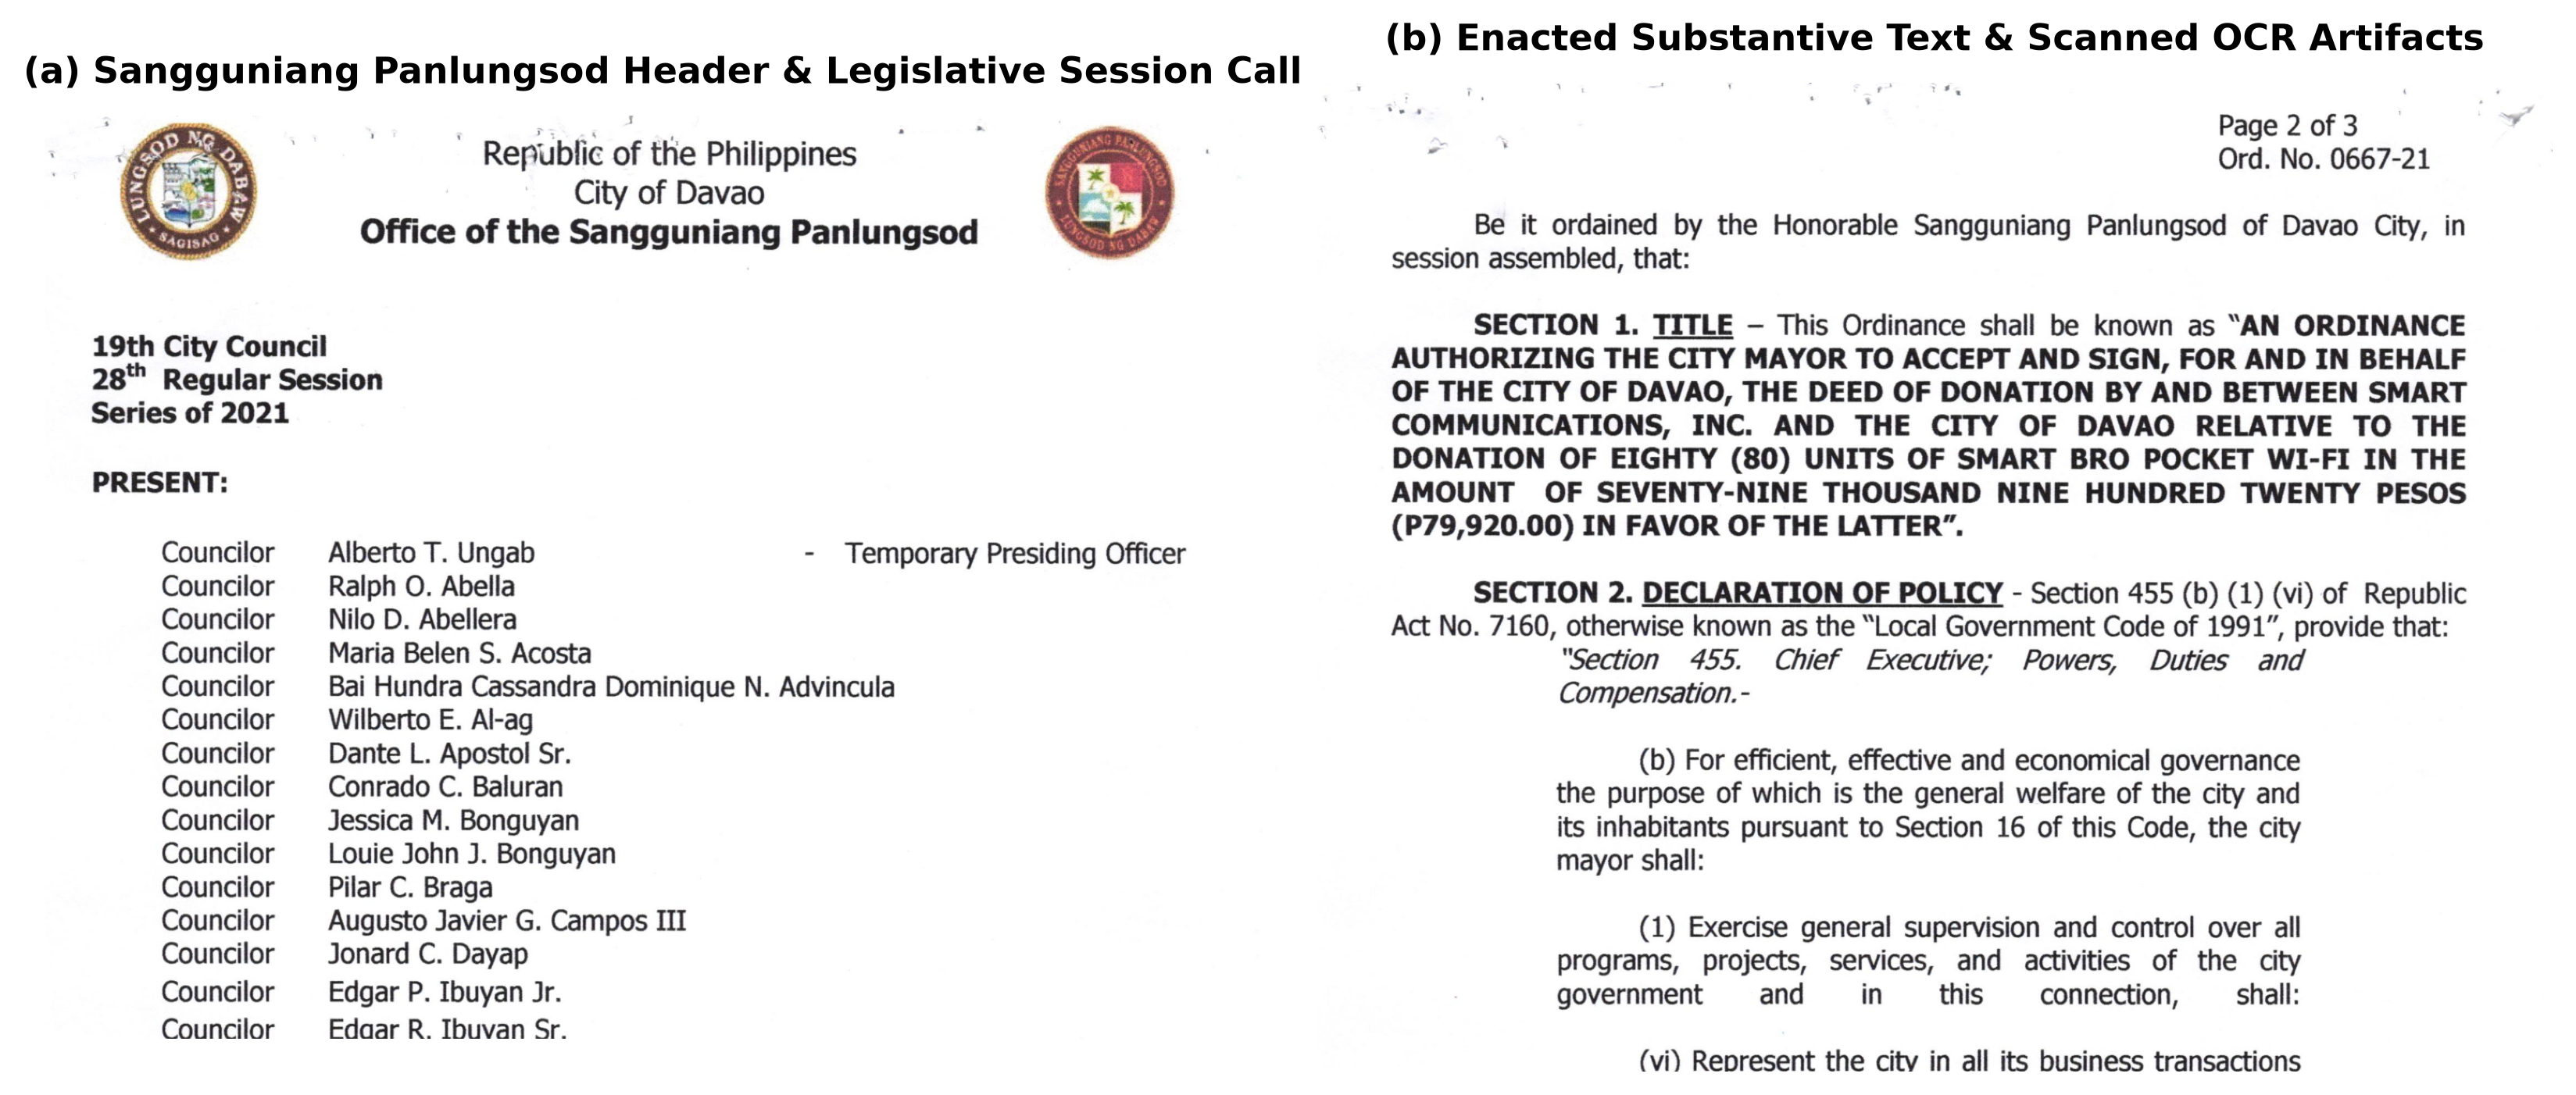
\includegraphics[width=0.96\linewidth]{figs/davao_ordinance_scan_sample.png}
            \caption{Sample Archival Document from the Davao City Sangguniang Panlungsod Corpus Illustrating Physical Scanning Artifacts and Optical Character Recognition (OCR) Noise. Panel (a) illustrates the official municipal session heading, seal, and city council metadata. Panel (b) shows the enacted substantive provisions exhibiting real OCR scanner noise, character substitutions (e.g., ``0667-2L'' for 2021, ``TITTE'' for Title), and document skew.}
            \label{fig:davao_ordinance_scan}
        \end{figure}

        In real-world legislation, direct contradictions between laws are very rare. Lawmakers generally try to write rules that work alongside existing higher laws rather than directly opposing them~\cite{fuller1964the}. As a result, actual legal conflicts make up less than 1\% of random pairs formed between municipal ordinances and national statutes. Taking random pairs of text from the unedited collections would lead to an overwhelming majority of unrelated pairs. A machine learning model trained on such unbalanced data could score 99\% nominal accuracy simply by guessing ``Neutral'' every time, while remaining unable to detect real legal conflicts.

        \subsubsection{Corpus Analysis}
        Across the five main types of legislation with sequential numbers, the collected corpus includes 19,683 statutes out of an estimated 20,246 historical laws, achieving a coverage rate of 97.22\%. When combined with the 5,749 Executive Orders from fifteen presidential administrations, the compiled national archive holds 25,432 out of about 26,451 total historical legal documents, reaching a national recall rate of 96.15\%. All official legislative totals reflect the chronological numbering sequence established by Congress and presidential records as of \textbf{March 2026}, where sequential Republic Acts reached Republic Act No.~12,313. Table~\ref{tab:statute_type_composition} provides a breakdown of the national corpus, comparing the collected documents with official legislative totals for each statutory type. Figure~\ref{fig:statute_type_composition} shows the share of each legal instrument in the archive, illustrating the large volume of executive orders alongside congressional acts.

        A key methodological decision in compiling this database is the explicit inclusion of \textbf{Executive Orders (EOs)} alongside congressional legislation. Under Article~VII, Section~17 of the 1987 Philippine Constitution and Book~III, Title~I, Chapter~2, Section~2 of the Administrative Code of 1987 (Executive Order No.~292)~\cite{philgov1987eo292}, Executive Orders are presidential acts providing rules of a general or permanent character in implementation or execution of constitutional or statutory mandates. Unlike Supreme Court decisions—which function as \textit{ex-post} judicial dispute resolutions settling private adversarial controversies under the doctrine of \textit{stare decisis} (Article~8, Civil Code)—Executive Orders operate as \textit{ex-ante}, forward-looking statutory instruments possessing the full force and effect of law. Furthermore, during both the Martial Law period (1972--1986) and the Revolutionary Government under the Freedom Constitution (Proclamation No.~3, 1986--1987), the President exercised direct legislative decree-making powers, enacting substantive national rules that remain active law today. Modern Executive Orders establish binding nationwide regulatory mandates—such as Executive Order No.~26 (s.~2017) mandating nationwide public smoking bans, or Executive Order No.~168 (s.~2014) creating the IATF with binding quarantine standards—that legally preempt inconsistent local ordinances. Excluding Executive Orders would create an artificial regulatory vacuum, allowing local ordinances to contradict operative presidential mandates.

        \begin{table}[!htbp]
            \centering
            \footnotesize
            \setlength{\tabcolsep}{3.8pt}
            \caption{Comparative Statutory Coverage and Composition of the Philippine National Legal Archive ($N = 25,432$)}
            \label{tab:statute_type_composition}
            \begin{tabularx}{\linewidth}{c>{\RaggedRight}p{2.85cm}rrrr>{\RaggedRight}X}
                \toprule
                \textbf{ID} & \shortstack[l]{\textbf{Statutory}\\\textbf{Instrument}} & \textbf{Corpus} & \shortstack[r]{\textbf{Official}\\\textbf{Total}} & \shortstack[r]{\textbf{Coverage}\\\textbf{Rate}} & \shortstack[r]{\textbf{Corpus}\\\textbf{Share}} & \textbf{Historical Era and Governing Authority} \\
                \midrule
                01 & Republic Acts (RA) & 11,963 & 12,313 & 97.16\% & 47.04\% & Post-war and Fifth Republic legislation (1946--present, up to RA 12313 as of March 2026) \\
                02 & Executive Orders (EO) & 5,749 & 6,205\textsuperscript{*} & 92.65\% & 22.61\% & Presidential administrative issuances (1901--2026, across 15 administrations) \\
                03 & Acts & 4,257 & 4,275 & 99.58\% & 16.74\% & American Insular Government enactments (1900--1935) \\
                04 & Presidential Decrees (PD) & 1,844 & 2,036 & 90.57\% & 7.25\% & Martial law legislative decrees enacted by executive fiat (1972--1986) \\
                05 & Batas Pambansa (BP) & 886 & 889 & 99.66\% & 3.48\% & Unicameral parliamentary legislation under the 1973 Constitution \\
                06 & Commonwealth Acts (CA) & 733 & 733 & 100.00\% & 2.88\% & Transitional governance enactments under the 1935 Constitution \\
                \midrule
                \multicolumn{2}{l}{\textbf{Sequential Subtotal}} & \textbf{19,683} & \textbf{20,246} & \textbf{97.22\%} & \textbf{77.39\%} & \textbf{All numbered legislative enactments of Congress} \\
                \multicolumn{2}{l}{\textbf{Total Archive}} & \textbf{25,432} & \textbf{26,451} & \textbf{96.15\%} & \textbf{100.00\%} & \textbf{Comprehensive corpus extracted from the Lawphil Project} \\
                \bottomrule
                \multicolumn{7}{p{0.97\linewidth}}{\scriptsize \textsuperscript{*}Historical total for Executive Orders represents the aggregate sum of maximum numbered issuances across all fifteen presidential administrations (1935--2026) and colonial governorships (1901--1935) as recorded in the Official Gazette and Lawphil archives as of March 2026.}
            \end{tabularx}
        \end{table}

        \begin{figure}[!htbp]
            \centering
            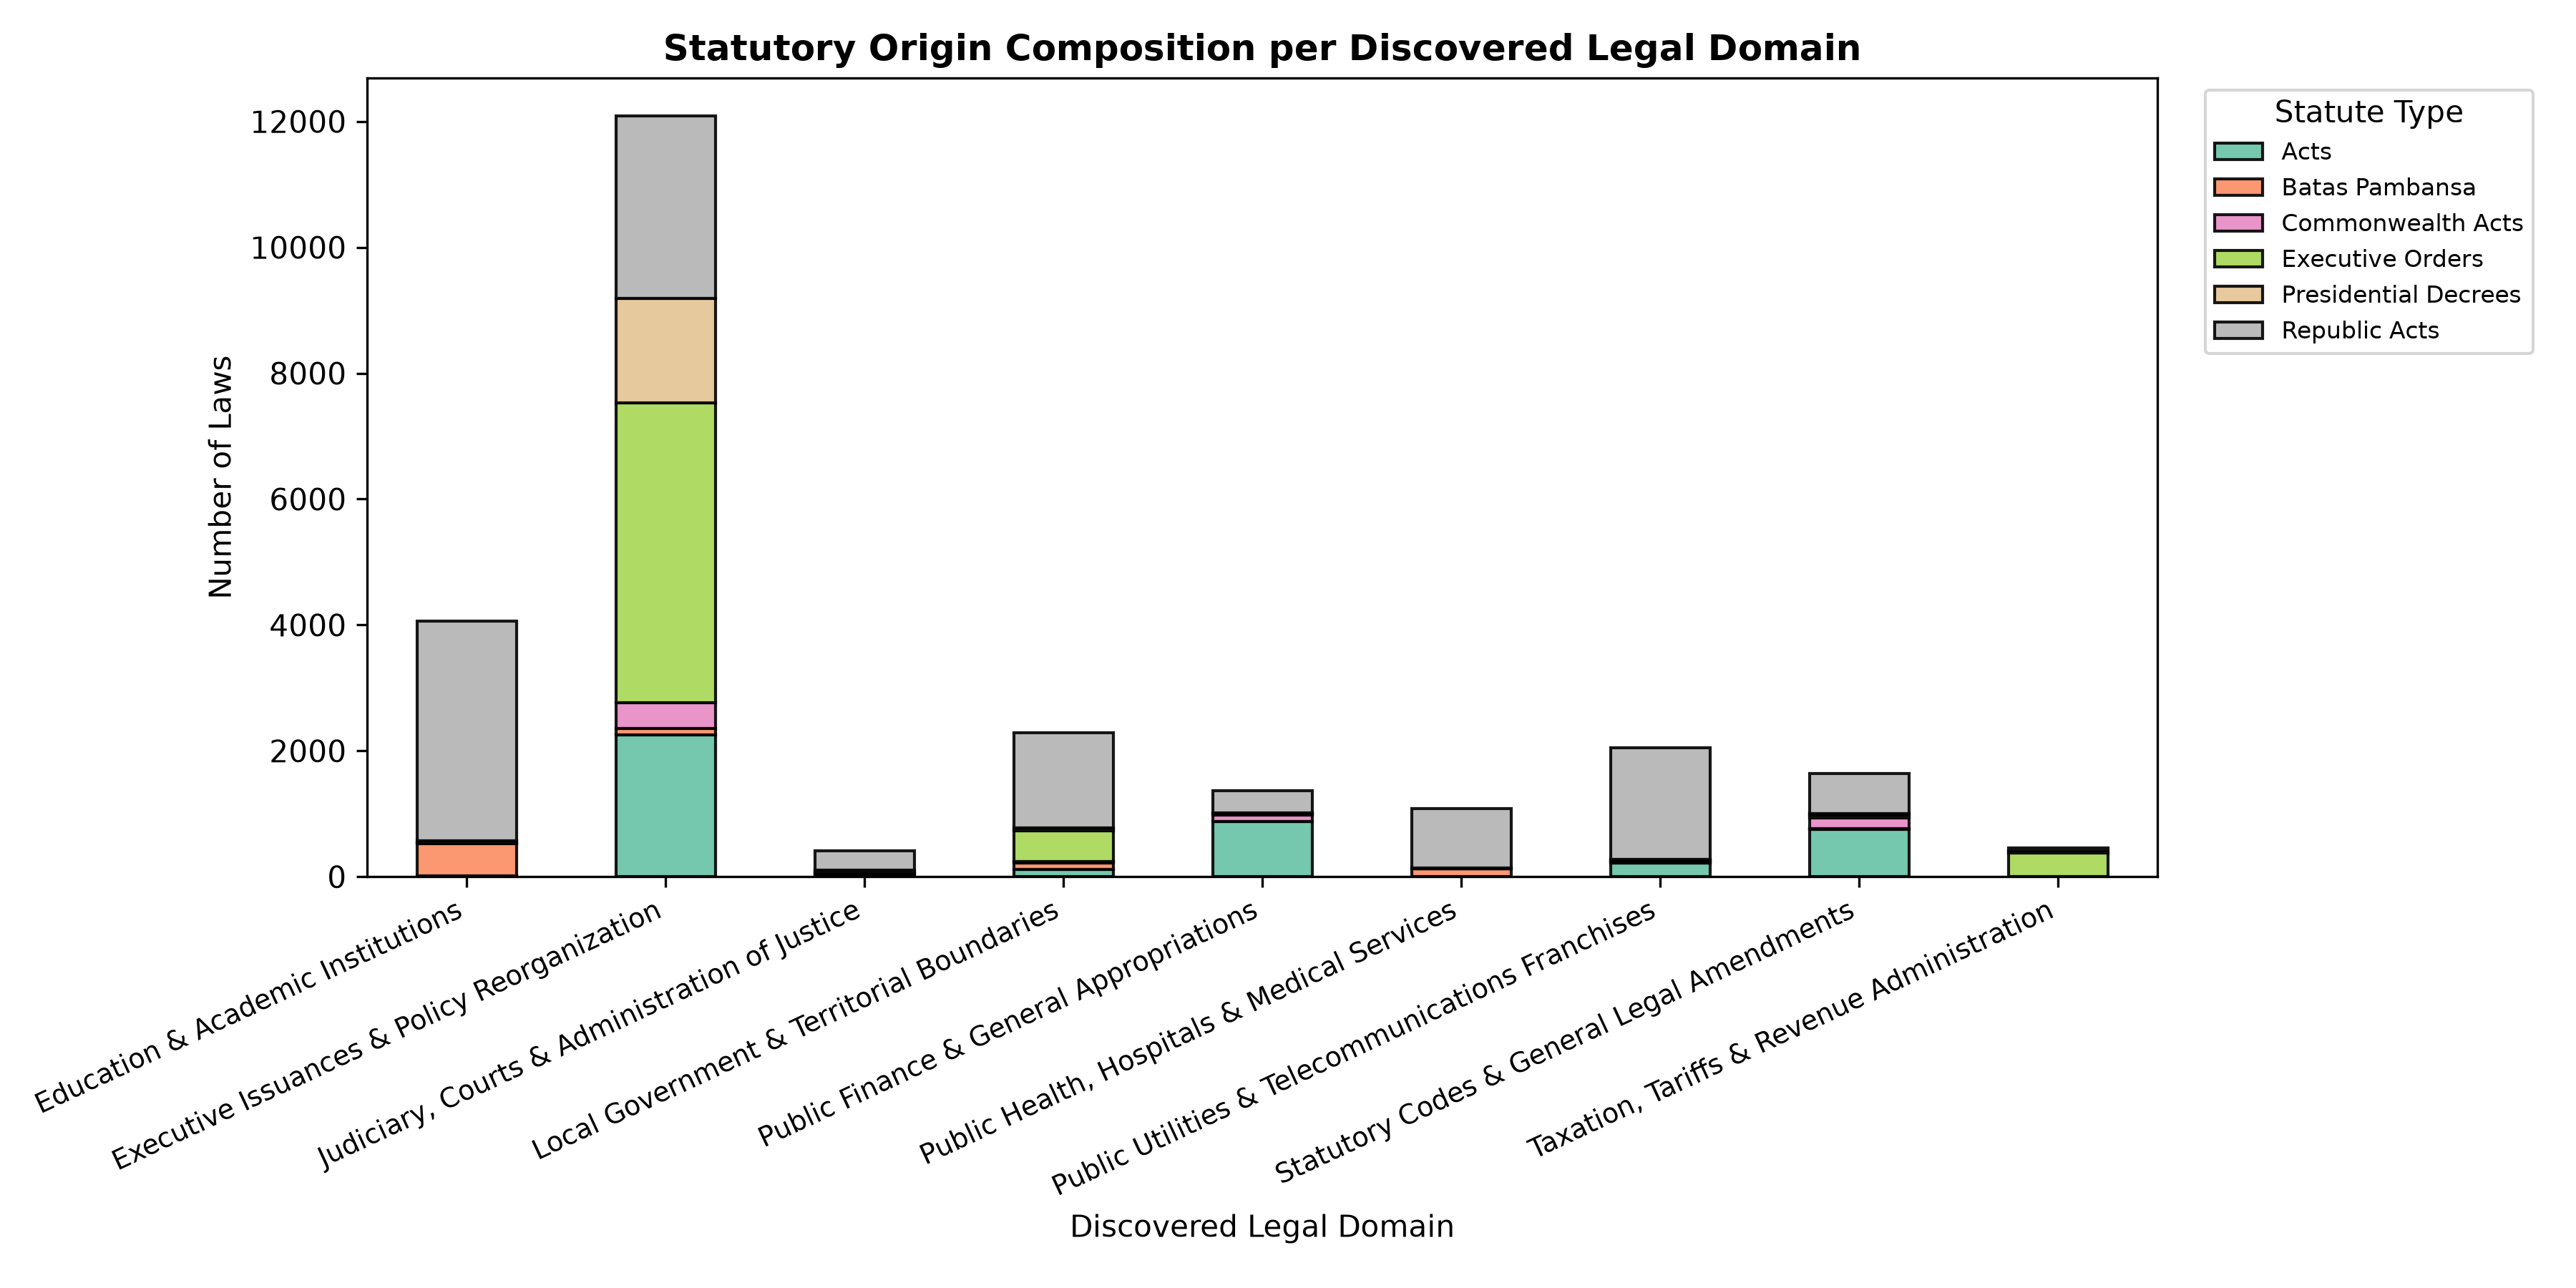
\includegraphics[width=0.78\linewidth]{figs/statute_type_composition.png}
            \caption{Composition of the Philippine National Statutory Corpus by Legislative Instrument ($N = 25,432$).}
            \label{fig:statute_type_composition}
        \end{figure}

        The coverage rates confirm that the national legal archive is nearly complete. Commonwealth Acts show full 100.00\% coverage across all 733 enactments, while American-era Acts (99.58\%) and Batas Pambansa (99.66\%) miss only 18 and 3 enactments, respectively. For Republic Acts, the 11,963 collected records cover 97.16\% of the 12,313 official total, with missing entries mainly being local bills or recent laws still being indexed. For Presidential Decrees, the 1,844 gathered records represent 90.57\% of the 2,036 numbered decrees from the Martial Law period, where uncollected entries were unpublished directives until the Supreme Court required full publication in \textit{Tañada v. Tuvera}~\cite{sc1985tanadavtuvera}. For Executive Orders, the 5,749 collected records represent 92.65\% of the 6,205 numbered orders issued across fifteen presidential terms, offering an extensive record of administrative policy.

        This breakdown also explains why executive and administrative orders account for nearly half (48.01\%) of the subsequent topic groups. Executive Orders (22.61\%) and Presidential Decrees (7.25\%) together make up 7,593 documents, representing nearly one-third of the entire national archive. When combined with colonial-era civil administration Acts and agency reorganizations, administrative directives form the largest single category of Philippine legal text. In language processing, this large volume of administrative text poses a challenge during search, as queries can easily match routine bureaucratic language rather than municipal regulations. This reality shows why automated topic grouping is needed to keep local ordinance checks focused on relevant laws.

        To trace how the six statutory instruments evolved across Philippine jurisprudence, the proponents categorized statutory enactments across six chronological eras. Each historical era established distinct legislative authorities, ranging from colonial commissions to modern constitutional congresses. Figure~\ref{fig:historical_temporal_evolution} charts the chronological succession and aggregate volume of statutory instruments from 1900 through 2026. The distribution reflects the shifting primacy of legislative acts, presidential decrees, and administrative executive orders across political transitions. Examining these enactment waves illustrates how historical governance structures directly shaped the composition of the national legal corpus.

        \begin{figure}[htbp]
            \centering
            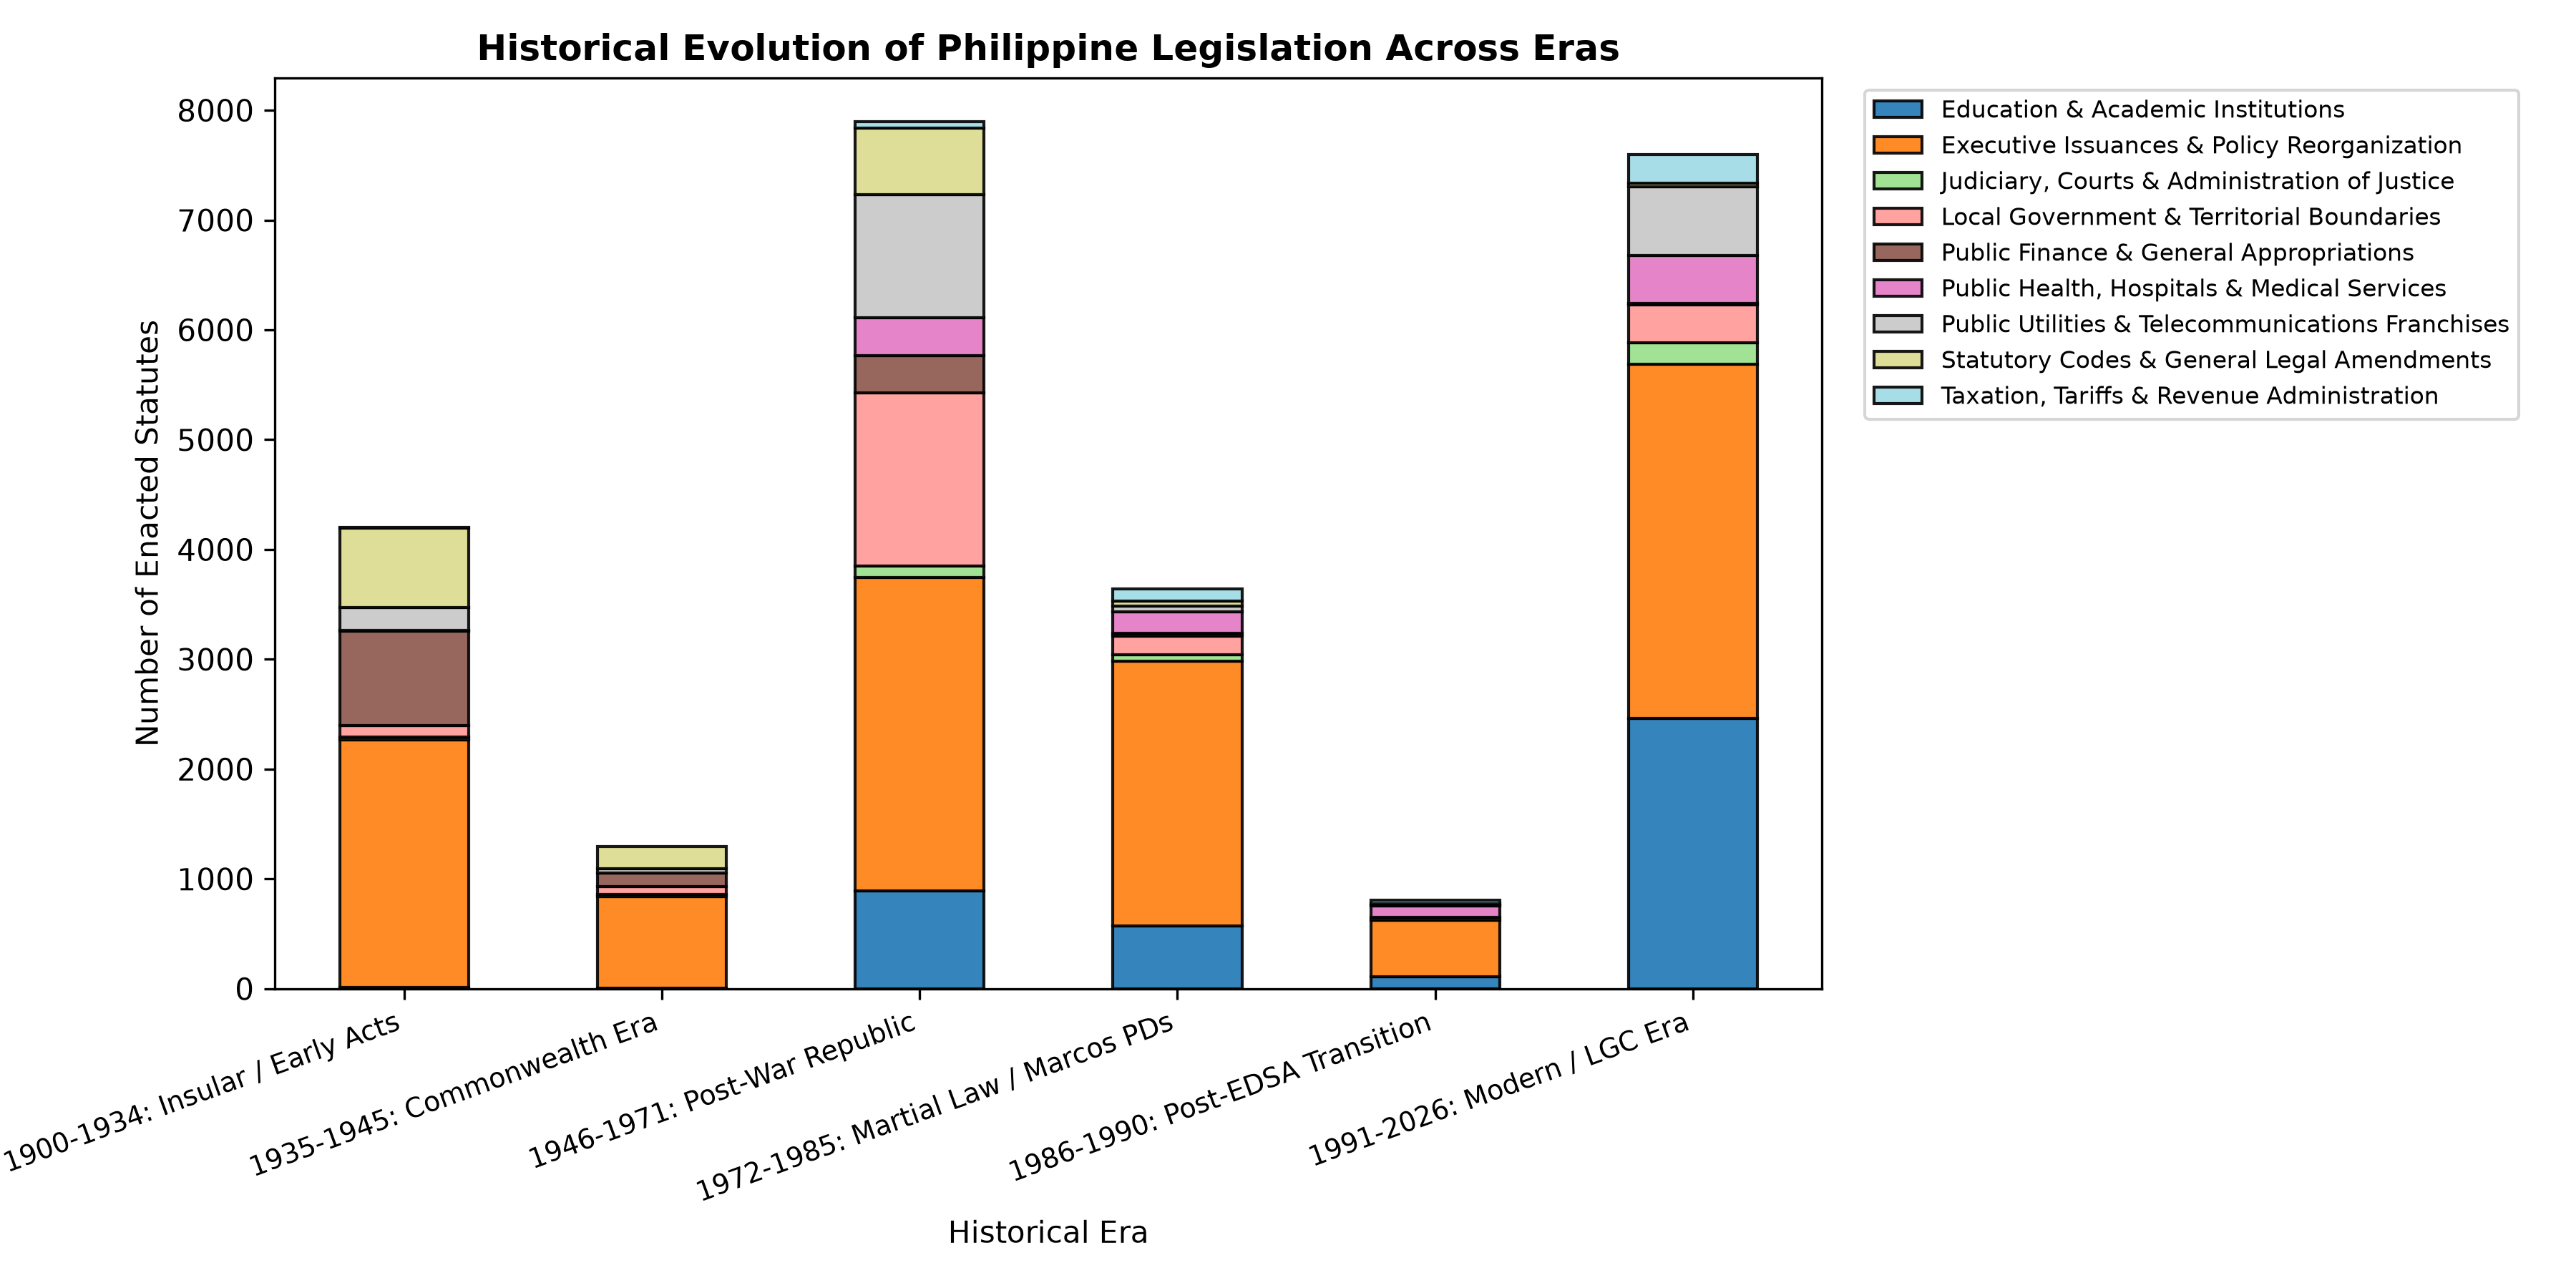
\includegraphics[width=0.96\linewidth]{figs/historical_temporal_evolution.png}
            \caption{Historical Succession and Volume of Statutory Instruments across Six Chronological Eras (1900--2026, $N = 25,432$).}
            \label{fig:historical_temporal_evolution}
        \end{figure}

        The temporal breakdown reveals that Philippine lawmaking expanded during periods of national administrative reorganization. Early colonial governance relied entirely on 4,199 foundational Acts during the Insular period (1900--1934). Centralized presidential lawmaking predominated during the Martial Law period through 1,844 Presidential Decrees and 886 Batas Pambansa parliamentary enactments (1972--1985). In the modern era governed by Republic Act No.~7160 (1991--2026), statutory production stabilized into a dual stream of 4,900 congressional Republic Acts and 2,421 executive policy orders. Because vocabulary standards shifted markedly across these legislative transitions, search models require chronological awareness to avoid misinterpreting historical statutory phrasing.

    \subsection{Preprocessing and Filtering}
    \label{sec:preprocessing_filtering}
    Because the raw downloaded files vary widely in formatting, they require thorough cleaning, grouping, and text normalization. While national statutes are already available as clean digital text, the scanned Davao City ordinances contain most of the OCR errors in the dataset. Since these local records come from image-based PDFs, extracting the text often produces misread characters and broken lines. The pipeline uses rule-based filters to find and correct these errors specifically within the local ordinance files. This targeted cleaning ensures that the subsequent vector conversion process is not disrupted by broken words or garbled text.

        \subsubsection{Digital-Born Draft Ingestion and Section Segmentation}
        \label{sec:draft_ingestion_segmentation}
        A critical operational distinction in this research separates the historical training archive from live ex-ante draft submissions. While the historical Davao City collection (~1,660 enactments from 1946 to 2025) consists of scanned physical PDFs requiring intensive optical character recognition (OCR) and text normalization, newly drafted ordinances submitted for ex-ante review are digital-born documents. Legislative staff create these proposed measures using standard word processing software, generating clean electronic text or searchable PDF files. Because digital-born drafts contain authentic character encodings without scanning artifacts, the live pipeline bypasses OCR error correction entirely. This structural decoupling allows the preprocessor to focus immediately on automated section boundary parsing and clause segmentation.

        To evaluate legislative commands without semantic distortion, an automated regular expression parser splits the submitted draft at formal section boundaries into discrete operative blocks. In Philippine local legislative practice, proposed measures follow standardized structural templates established by the Department of the Interior and Local Government~\cite{dilg2022drafting}. However, real-world legislative drafts contain substantial procedural boilerplate that does not express substantive legal commands. If routine clauses such as title declarations, repealing clauses, and effectivity dates are fed into Stage~1 retrieval, they match thousands of administrative national statutes containing similar formulaic phrases. To prevent search drift and computational waste, the preprocessor automatically filters out non-operative sections---specifically Title, Separability, Repealing, and Effectivity clauses---directing candidate retrieval exclusively toward substantive regulatory and penal provisions.

        Listing~\ref{lst:jsonl_sample} displays an authentic raw ingestion record from the scraped national statutory collection (\texttt{corpus/national\_laws/republic\_acts.jsonl}), capturing the raw unparsed text, enactment year, and source URL for Republic Act No.~11035 (\textit{Balik Scientist Act}, matching the Lawphil page illustrated in Figure~\ref{fig:lawphil_web_interface}). Listing~\ref{lst:provision_extractor} details the regular expression parser that segments live draft measures into discrete operative sections while filtering out procedural boilerplate.

        \begin{lstlisting}[language=Python, caption={Sample Raw JSONL Ingestion Record from the National Statutory Archive (Republic Act No. 11035)}, label={lst:jsonl_sample}]
# Raw Ingestion Record from corpus/national_laws/republic_acts.jsonl (ra_11035_2018)
raw_statute_record = {
    "law_id": "ra_11035_2018",
    "year": 2018,
    "url": "https://lawphil.net/statutes/repacts/ra2018/ra_11035_2018.html",
    "scraped_at": "2026-02-17T18:44:04.745654",
    "text": (
        "Seventeenth Congress\nSecond Regular Session\nBegun and held in Metro Manila, "
        "on Monday, the twenty-fourth day of July, two thousand seventeen.\n"
        "REPUBLIC ACT No. 11035\n"
        "An Act Institutionalizing the Balik Scientist Program, Appropriating Funds "
        "Therefor, and for Other Purpose\n"
        "Be it enacted by the Senate and House of Representatives of the Philippines "
        "in Congress assembled:\n"
        "Section 1. Title. - This Act shall be known as the \"Balik Scientist Act.\"\n"
        "Section 2. Declaration of Policy. - The State recognizes that the utilization "
        "of the expertise of science, technology or innovation experts of Filipino descent "
        "is a vital component of the national political, economic, and social development "
        "efforts...\n"
        "Section 3. Balik Scientist Program. - There is hereby created a Balik Scientist "
        "Program, hereinafter referred to as the \"Program\", to be administered by the "
        "Department of Science and Technology (DOST)...\n"
        "[Raw statutory text continues across 2,493 total words]"
    )
}
        \end{lstlisting}

        \begin{lstlisting}[language=Python, caption={Code Snippet of the Operative Provision Extractor and Boilerplate Filter}, label={lst:provision_extractor}]
import re

def extract_operative_provisions(draft_text):
    """
    Parses digital-born draft ordinance into discrete sections,
    filtering out non-operative procedural boilerplate clauses.
    """
    # Regex pattern to segment text at formal section boundaries
    pattern = r'(SECTION\s+\d+\.?[^\n]*\n.*?)(?=(?:SECTION\s+\d+|CERTIFIED|ENACTED|\Z))'
    matches = re.findall(pattern, draft_text, re.DOTALL | re.IGNORECASE)
    
    # Procedural clauses that do not carry substantive regulatory commands
    boilerplate_keywords = ["TITLE", "SEPARABILITY", "REPEALING", "EFFECTIVITY"]
    operative_sections = []
    
    for match in matches:
        clean_chunk = ' '.join(match.strip().split())
        header = clean_chunk.split('.')[0] if '.' in clean_chunk else clean_chunk[:30]
        
        # Exclude non-operative procedural boilerplate
        if any(kw in header.upper() for kw in boilerplate_keywords):
            continue
            
        operative_sections.append({
            "section_header": header,
            "operative_text": clean_chunk
        })
        
    return operative_sections
        \end{lstlisting}

        Once operative sections are isolated, evaluating granular statutory provisions requires preserving their governing legislative identity. An isolated sub-clause (such as a standalone penalty statement) stripped of its parent enactment number and title suffers from severe semantic vector dilution, causing retrieval models to confuse municipal regulatory penalties with unrelated national tax or criminal codes. To maintain semantic precision and hierarchy across both stages, the pipeline applies structural context prepending. Listing~\ref{lst:context_prepending} details the context prepending protocol, while Listing~\ref{lst:model_ready_chunk} demonstrates the concrete transformation from an isolated provision into a Stage~1 indexed chunk and the resulting Stage~2 asymmetric input sequence.

        \begin{lstlisting}[language=Python, caption={Pseudocode of the Section Context Prepending Protocol for Granular Provision Chunking}, label={lst:context_prepending}]
def prepend_statutory_context(statute_record, section):
    """
    Prepends governing legislative identity to isolated section text
    to prevent semantic vector dilution and preserve hierarchical rank.
    """
    prefix = (
        f"[{statute_record['instrument_type']} No. {statute_record['enactment_number']}: "
        f"{statute_record['title']} | {section['section_number']}: {section['section_title']}] "
    )
    model_ready_text = prefix + section['raw_text']
    return model_ready_text
        \end{lstlisting}

        \begin{lstlisting}[language=Python, caption={Sample Model-Ready Statutory Chunk and Stage 2 Input Sequence with Context Prepending}, label={lst:model_ready_chunk}]
# 1. Isolated Statutory Provision (Without Context Prepending)
# Lacks parent statutory identity; dense embeddings match ambiguous administrative powers.
isolated_section = (
    "Section 458. (a) The sangguniang panlungsod, as the legislative body of the city, "
    "shall enact ordinances... (v) Approve ordinances which shall impose a fine not "
    "exceeding Five thousand pesos (P5,000.00) or an imprisonment not exceeding one (1) "
    "year, or both."
)

# 2. Model-Ready Contextualized Provision Chunk (Indexed by Stage 1 BM25 & Dense Bi-Encoders)
# Prepends statutory title and citation to establish legal hierarchy and topical specificity.
stage1_indexed_chunk = (
    "[Republic Act No. 7160: Local Government Code of 1991 | Section 458: Powers, Duties, "
    "and Functions of the Sangguniang Panlungsod] Section 458. (a) The sangguniang panlungsod, "
    "as the legislative body of the city, shall enact ordinances... (v) Approve ordinances which "
    "shall impose a fine not exceeding Five thousand pesos (P5,000.00) or an imprisonment not "
    "exceeding one (1) year, or both."
)

# 3. Assembled Asymmetric Input Sequence Passed to Stage 2 Cross-Encoder
# Formatted with [CLS] and [SEP] tokens pairing governing premise with proposed draft hypothesis.
stage2_input_sequence = (
    "[CLS] Premise: [Republic Act No. 7160: Local Government Code of 1991 | Section 458: "
    "Powers of the Sangguniang Panlungsod] Section 458. (a)... Approve ordinances which shall "
    "impose a fine not exceeding Five thousand pesos (P5,000.00)... "
    "[SEP] Hypothesis: [Proposed Davao City Ordinance No. 2024-012 | Section 6: Penalties] "
    "SECTION 6. PENALTY CLAUSE. Any person violating this Ordinance shall be penalized with "
    "a fine of Fifteen Thousand Pesos (PHP 15,000.00) or two years imprisonment. [SEP]"
)
        \end{lstlisting}

        \subsubsection{Domain Categorization}
        \label{sec:domain_categorization}
        During preliminary exploratory research, the proponents conducted initial machine learning experiments on the national statutory archive and identified severe dataset imbalances. In the national collection of 25,432 statutes, routine executive issuances and administrative reorganizations comprise nearly half of all historical enactments, while specialized regulatory domains remain relatively small. Searching for a local regulatory ordinance across this raw, unfiltered collection causes severe search drift because dense retrieval models readily match repetitive administrative phrasing across unrelated legal areas. To resolve these dataset quirks, the proponents formalized a two-stage topic modeling architecture that organizes the statutory archive into cohesive, well-separated subject areas. This structured categorization prevents routine administrative directives from crowding the candidate shortlist during coarse retrieval, establishing a balanced foundation for subsequent conflict checks.

        The topic classification pipeline groups documents automatically while running smoothly on standard local computers. First, the 25,432 statutory texts are cleaned by removing HTML tags and routine metadata. The pipeline removes a custom list of 49 common legal stopwords, such as ``hereby,'' ``enacted,'' and ``republic,'' which appear in almost every law without helping identify its specific topic. Second, the cleaned texts are converted into term frequency-inverse document frequency (TF-IDF) feature vectors, capped at a vocabulary of 25,000 single words and two-word phrases. In text mining and information retrieval, TF-IDF is a statistical weighting that measures the relative importance of a term within a document relative to an entire corpus; it rewards words that appear frequently within a particular statute while penalizing ubiquitous terms that appear indiscriminately across the broader archive~\cite{manning2008introduction}. To keep calculations fast on local hardware while preserving conceptual cohesion, the pipeline uses Truncated Singular Value Decomposition (SVD) to project the sparse word vectors into 64 latent semantic dimensions~\cite{deerwester1990indexing}. In latent semantic modeling, Landauer et al.~\cite{landauer1998introduction} established that projecting vocabulary matrices into a 50-to-300 dimensional latent subspace captures underlying semantic associations while filtering out high-frequency lexical noise and idiosyncratic drafting variations. This is followed by standard $L_2$ vector normalization.

        Grouping legal texts directly into a small number of broad topics risks mixing very different types of laws together. To avoid this problem, the normalized 64-dimensional vectors are first divided into $K = 28$ smaller micro-clusters using MiniBatch $K$-Means clustering~\cite{sculley2010webscale}. Following the over-clustering strategy recommended by Grootendorst~\cite{grootendorst2022bertopic} and Aggarwal~\cite{aggarwal2012mining}, setting an over-complete cluster space ($K \approx 20\text{--}30$) isolates repetitive narrow enactments, such as school conversions or telecom franchises, into tight individual clusters before macro consolidation. Next, the pipeline adapts the class-based TF-IDF ($c\text{-}TF\text{-}IDF$) method from Grootendorst~\cite{grootendorst2022bertopic} to find the most representative keywords for each group. By treating all text within a micro-cluster as a single combined document, $c\text{-}TF\text{-}IDF$ measures how important a word is to that specific cluster compared to the rest of the collection:

        \[
            c\text{-}TF\text{-}IDF_{i, c} = \frac{|t_{i, c}|}{|c|} \times \log\left(1 + \frac{A}{\sum_{k} |t_{i, k}|}\right)
        \]
        where $|t_{i, c}|$ represents the absolute frequency of word $i$ within cluster $c$, $|c|$ denotes the total word count of cluster $c$, and $A$ indicates the mean word count per cluster across the full collection.

        In order to connect these mathematical clusters to real legal subjects, the extracted $c\text{-}TF\text{-}IDF$ keywords are matched against a curated Philippine legal taxonomy. This taxonomy reflects the main local government duties and regulatory powers outlined in the Local Government Code of 1991~\cite{philgov1991ra7160}. Micro-clusters that share the same general legal topic are merged into consolidated macro domains. To remove minor edge cases, the pipeline requires each macro domain to contain at least 1.0\% of the corpus ($N \ge 254$ statutes). Micro-clusters that fall below this cutoff are reassigned to their nearest semantic center, ensuring each macro domain has enough documents for reliable search indexing:

        \[
            \mathbf{C}_m = \frac{\sum_{i \in \mathcal{D}_m} \mathbf{z}_i}{\left\|\sum_{i \in \mathcal{D}_m} \mathbf{z}_i\right\|_2}, \quad P(m \mid \mathbf{z}_i) = \frac{\exp(\tau \cdot \cos(\mathbf{z}_i, \mathbf{C}_m))}{\sum_{j} \exp(\tau \cdot \cos(\mathbf{z}_i, \mathbf{C}_j))}
        \]
        where $\mathbf{z}_i$ represents the normalized 64-dimensional SVD vector of document $i$, $\mathbf{C}_m$ denotes the normalized centroid of macro domain $m$, and $\tau = 6.0$ functions as the inverse temperature scaling parameter governing prediction confidence. Adapting temperature scaling principles from Guo et al.~\cite{guo2017calibration}, this scaling factor prevents uncalibrated softmax dispersion across high-dimensional cosine distances, ensuring that dominant domain probabilities are sharply delineated without over-confident saturation.

        Running this topic grouping workflow across all 25,432 national statutes organizes the historical collection into eight Consolidated Macro Legal Domains. Table~\ref{tab:national_macro_domains} lists the final distribution, showing document counts, percentages, and the most descriptive keywords for each domain. Figure~\ref{fig:macro_domain_distribution} illustrates the relative size of each discovered macro domain.

        \begin{table}[htbp]
            \centering
            \footnotesize
            \caption{Consolidated Macro Legal Domains of the Philippine National Statutory Corpus ($N = 25,432$)}
            \label{tab:national_macro_domains}
            \begin{tabularx}{\linewidth}{r>{\RaggedRight}p{5.8cm}rr>{\RaggedRight}X}
                \toprule
                \textbf{ID} & \textbf{Consolidated Macro Domain} & \textbf{Statutes} & \textbf{Share} & \textbf{Top Salient $c\text{-}TF\text{-}IDF$ Keywords} \\
                \midrule
                00 & Executive Issuances \& Policy Reorganization & 12,210 & 48.01\% & executive, commission, committee, policy, code \\
                01 & Education \& Academic Institutions & 3,492 & 13.73\% & high school, elementary school, campus, college \\
                02 & Local Government \& Territorial Boundaries & 2,134 & 8.39\% & barangay, municipality, boundary, sitio, territorial \\
                03 & Public Utilities \& Telecom Franchises & 2,041 & 8.03\% & franchise, broadcast, telecommunications, radio \\
                04 & Public Health, Hospitals \& Medical Services & 1,890 & 7.43\% & hospital, bed capacity, medical center, infirmary \\
                05 & Statutory Codes \& General Legal Amendments & 1,873 & 7.36\% & administrative code, revised, amend, article, penalty \\
                06 & Public Finance \& General Appropriations & 1,335 & 5.25\% & appropriation, treasury, funds, expenditures \\
                07 & Taxation, Tariffs \& Revenue Administration & 457 & 1.80\% & tariff, customs code, internal revenue, excise \\
                \midrule
                \multicolumn{2}{l}{\textbf{Total Consolidated National Corpus}} & \textbf{25,432} & \textbf{100.00\%} & \textbf{All Enacted Statutes (1900--2026)} \\
                \bottomrule
            \end{tabularx}
        \end{table}

        \begin{figure}[htbp]
            \centering
            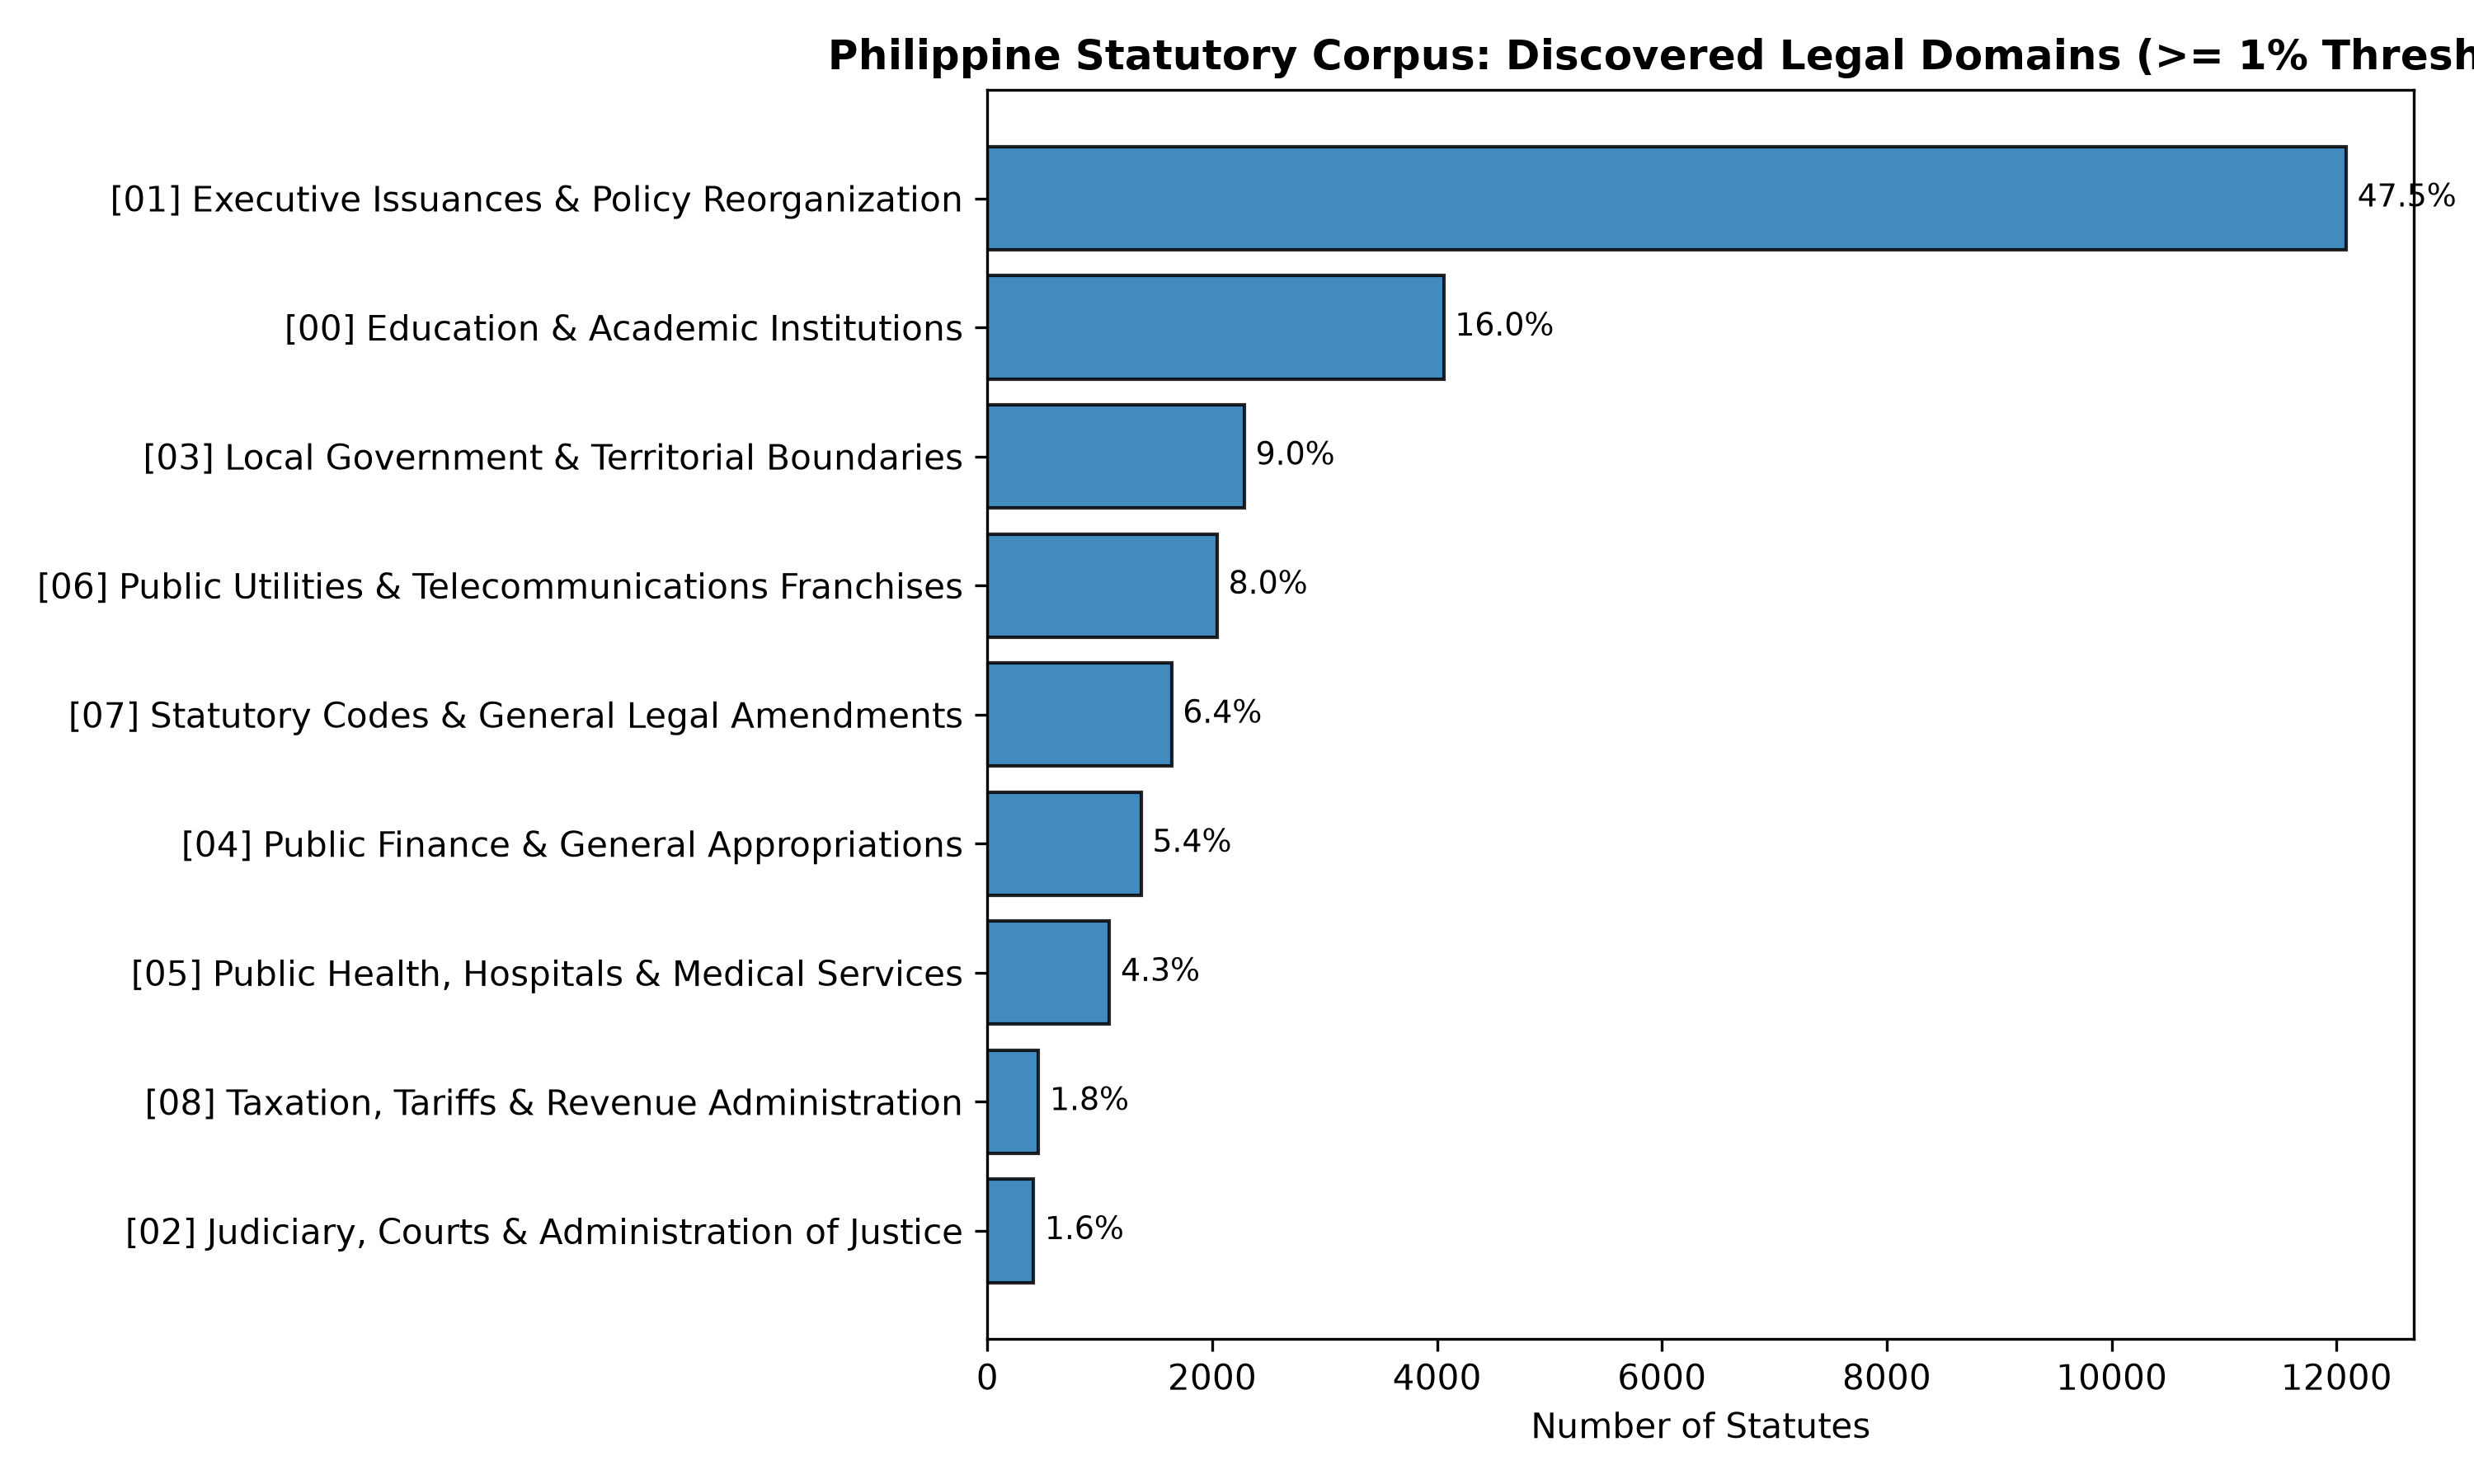
\includegraphics[width=0.88\linewidth]{figs/macro_domain_distribution.png}
            \caption{Distribution of the 25,432 Philippine National Statutes across the Consolidated Macro Legal Domains.}
            \label{fig:macro_domain_distribution}
        \end{figure}

        The topic distribution reflects the historical patterns of Philippine lawmaking. Executive issuances, administrative orders, and presidential decrees make up nearly half of the entire statutory collection, reflecting centralized authority during past political transitions. Common municipal subjects, including school infrastructure (13.73\%) and public utility franchises (8.03\%), form large distinct clusters with repetitive drafting patterns. In contrast, key regulatory topics like taxation (1.80\%) and public health (7.43\%) occupy smaller, highly focused portions of the database. Separating these regulatory clusters keeps routine administrative orders from crowding the candidate list during Stage~1 retrieval.

        To examine the geometric separation of these legal topics, the proponents projected the 64-dimensional SVD document vectors into a two-dimensional latent semantic landscape. Dimensionality reduction maps document similarities onto coordinate axes, allowing direct visual inspection of cluster cohesion. Figure~\ref{fig:semantic_topic_landscape_2d} illustrates this topic landscape across a representative stratified sample ($N = 3,500$), highlighting the core clusters and their spatial distributions.

        \begin{figure}[htbp]
            \centering
            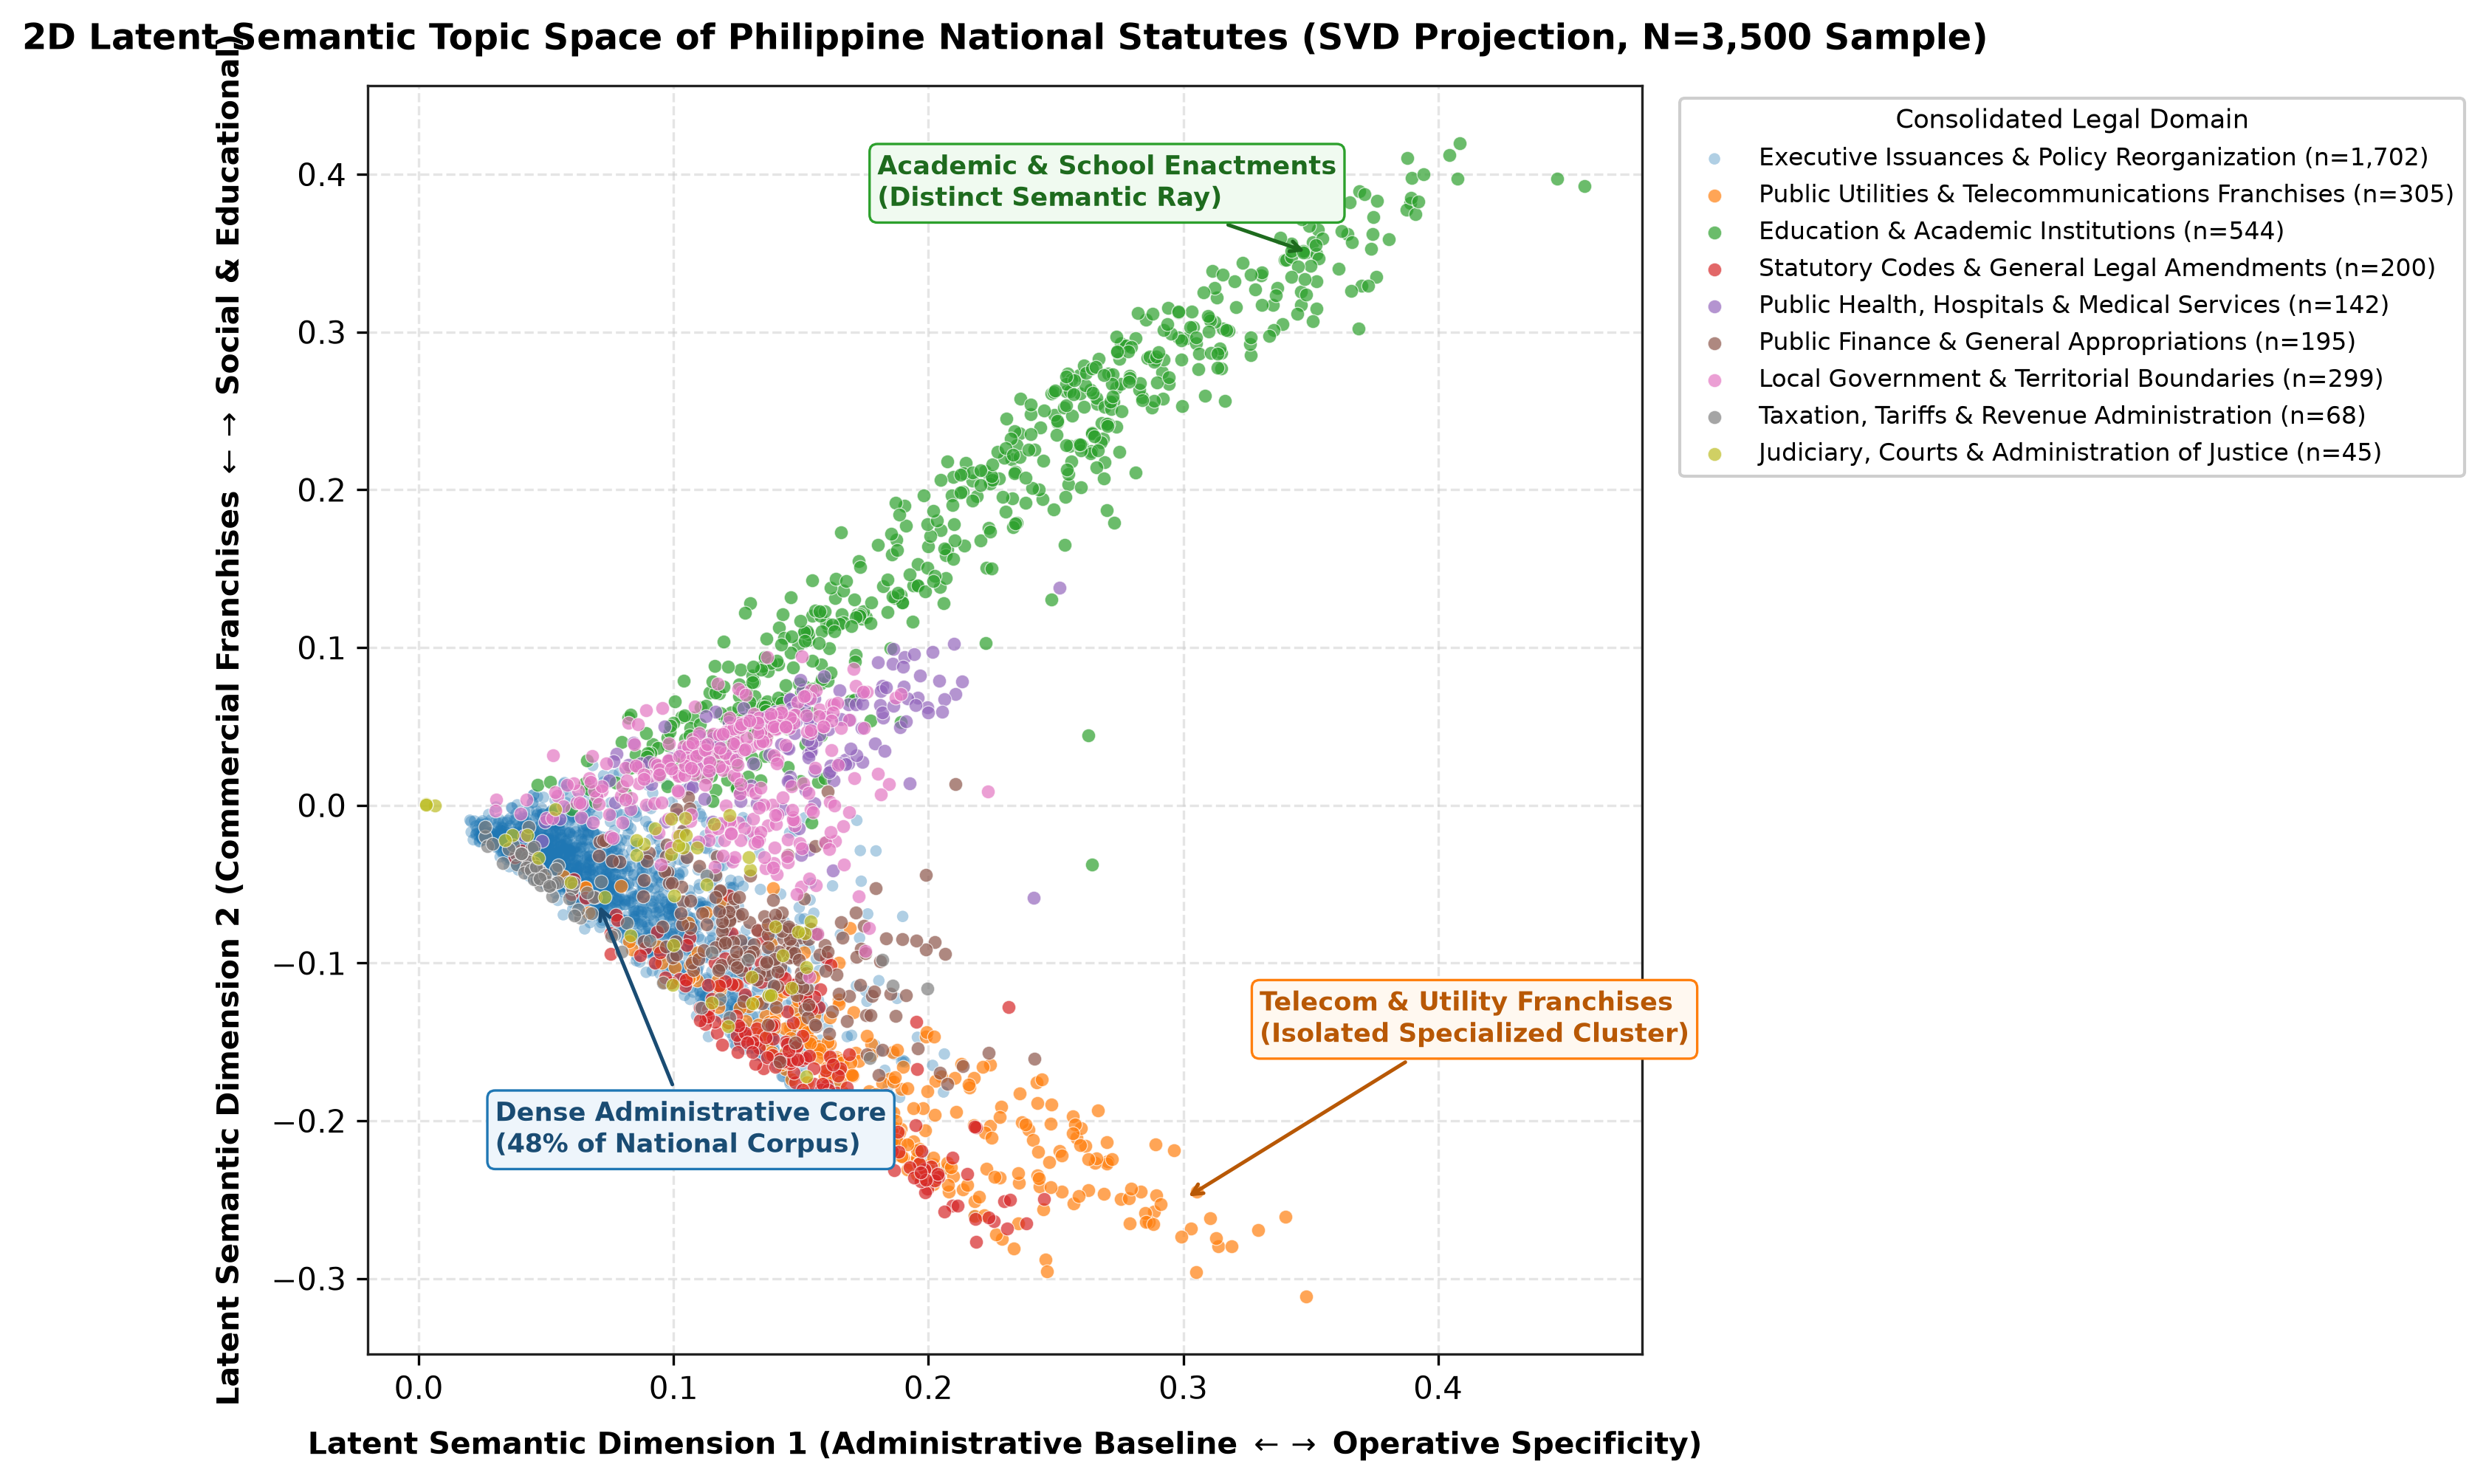
\includegraphics[width=0.92\linewidth]{figs/semantic_topic_landscape_2d.png}
            \caption{Two-Dimensional Latent Semantic Topic Space of the Philippine National Statutory Corpus (SVD Projection, $N = 3,500$ Representative Sample).}
            \label{fig:semantic_topic_landscape_2d}
        \end{figure}

        The two-dimensional semantic landscape reveals two distinct structural properties in Philippine statutory text. First, specialized regulatory domains project outward as distinct, isolated rays along the periphery of the vector space. Enactments establishing academic institutions and telecommunications franchises form tight, cohesive rays with minimal dispersion. In contrast, administrative issuances and executive orders cluster densely near the origin, comprising almost half of the entire archive. This dense central mass explains why unconstrained semantic searches frequently drift toward routine bureaucratic orders unless restrained by hierarchical safeguards.

        The coordinate axes reflect the two primary orthogonal directions of vocabulary variation discovered through singular value decomposition. The horizontal axis measures operative statutory specificity against general administrative phrasing, where higher positive values indicate detailed technical mandates rather than procedural orders. Conversely, the vertical axis captures functional divergence between social infrastructure such as public schools and commercial infrastructure such as telecommunications franchises. Although the dense cluster on the left appears visually compacted on a two-dimensional plane, the underlying MiniBatch $K$-Means clustering was performed in 64 dimensions where mathematical boundaries remain well-separated. Projecting 64 dimensions onto a flat plane inevitably collapses higher-order distinctions, yet this dense central mass visually demonstrates why unconstrained semantic retrieval suffers from search drift without domain filtering.

        To confirm that the mathematical clusters reflect substantive legal categories rather than shared administrative boilerplate, the proponents examined the most salient vocabulary terms discovered by the model. Words that appear frequently across all documents fail to differentiate legal topics, requiring class-based weightings to isolate subject matter. Figure~\ref{fig:top_keywords_per_domain} displays the top class-based TF-IDF ($c\text{-}TF\text{-}IDF$) keywords across all eight consolidated macro domains.

        \begin{figure}[!htbp]
            \centering
            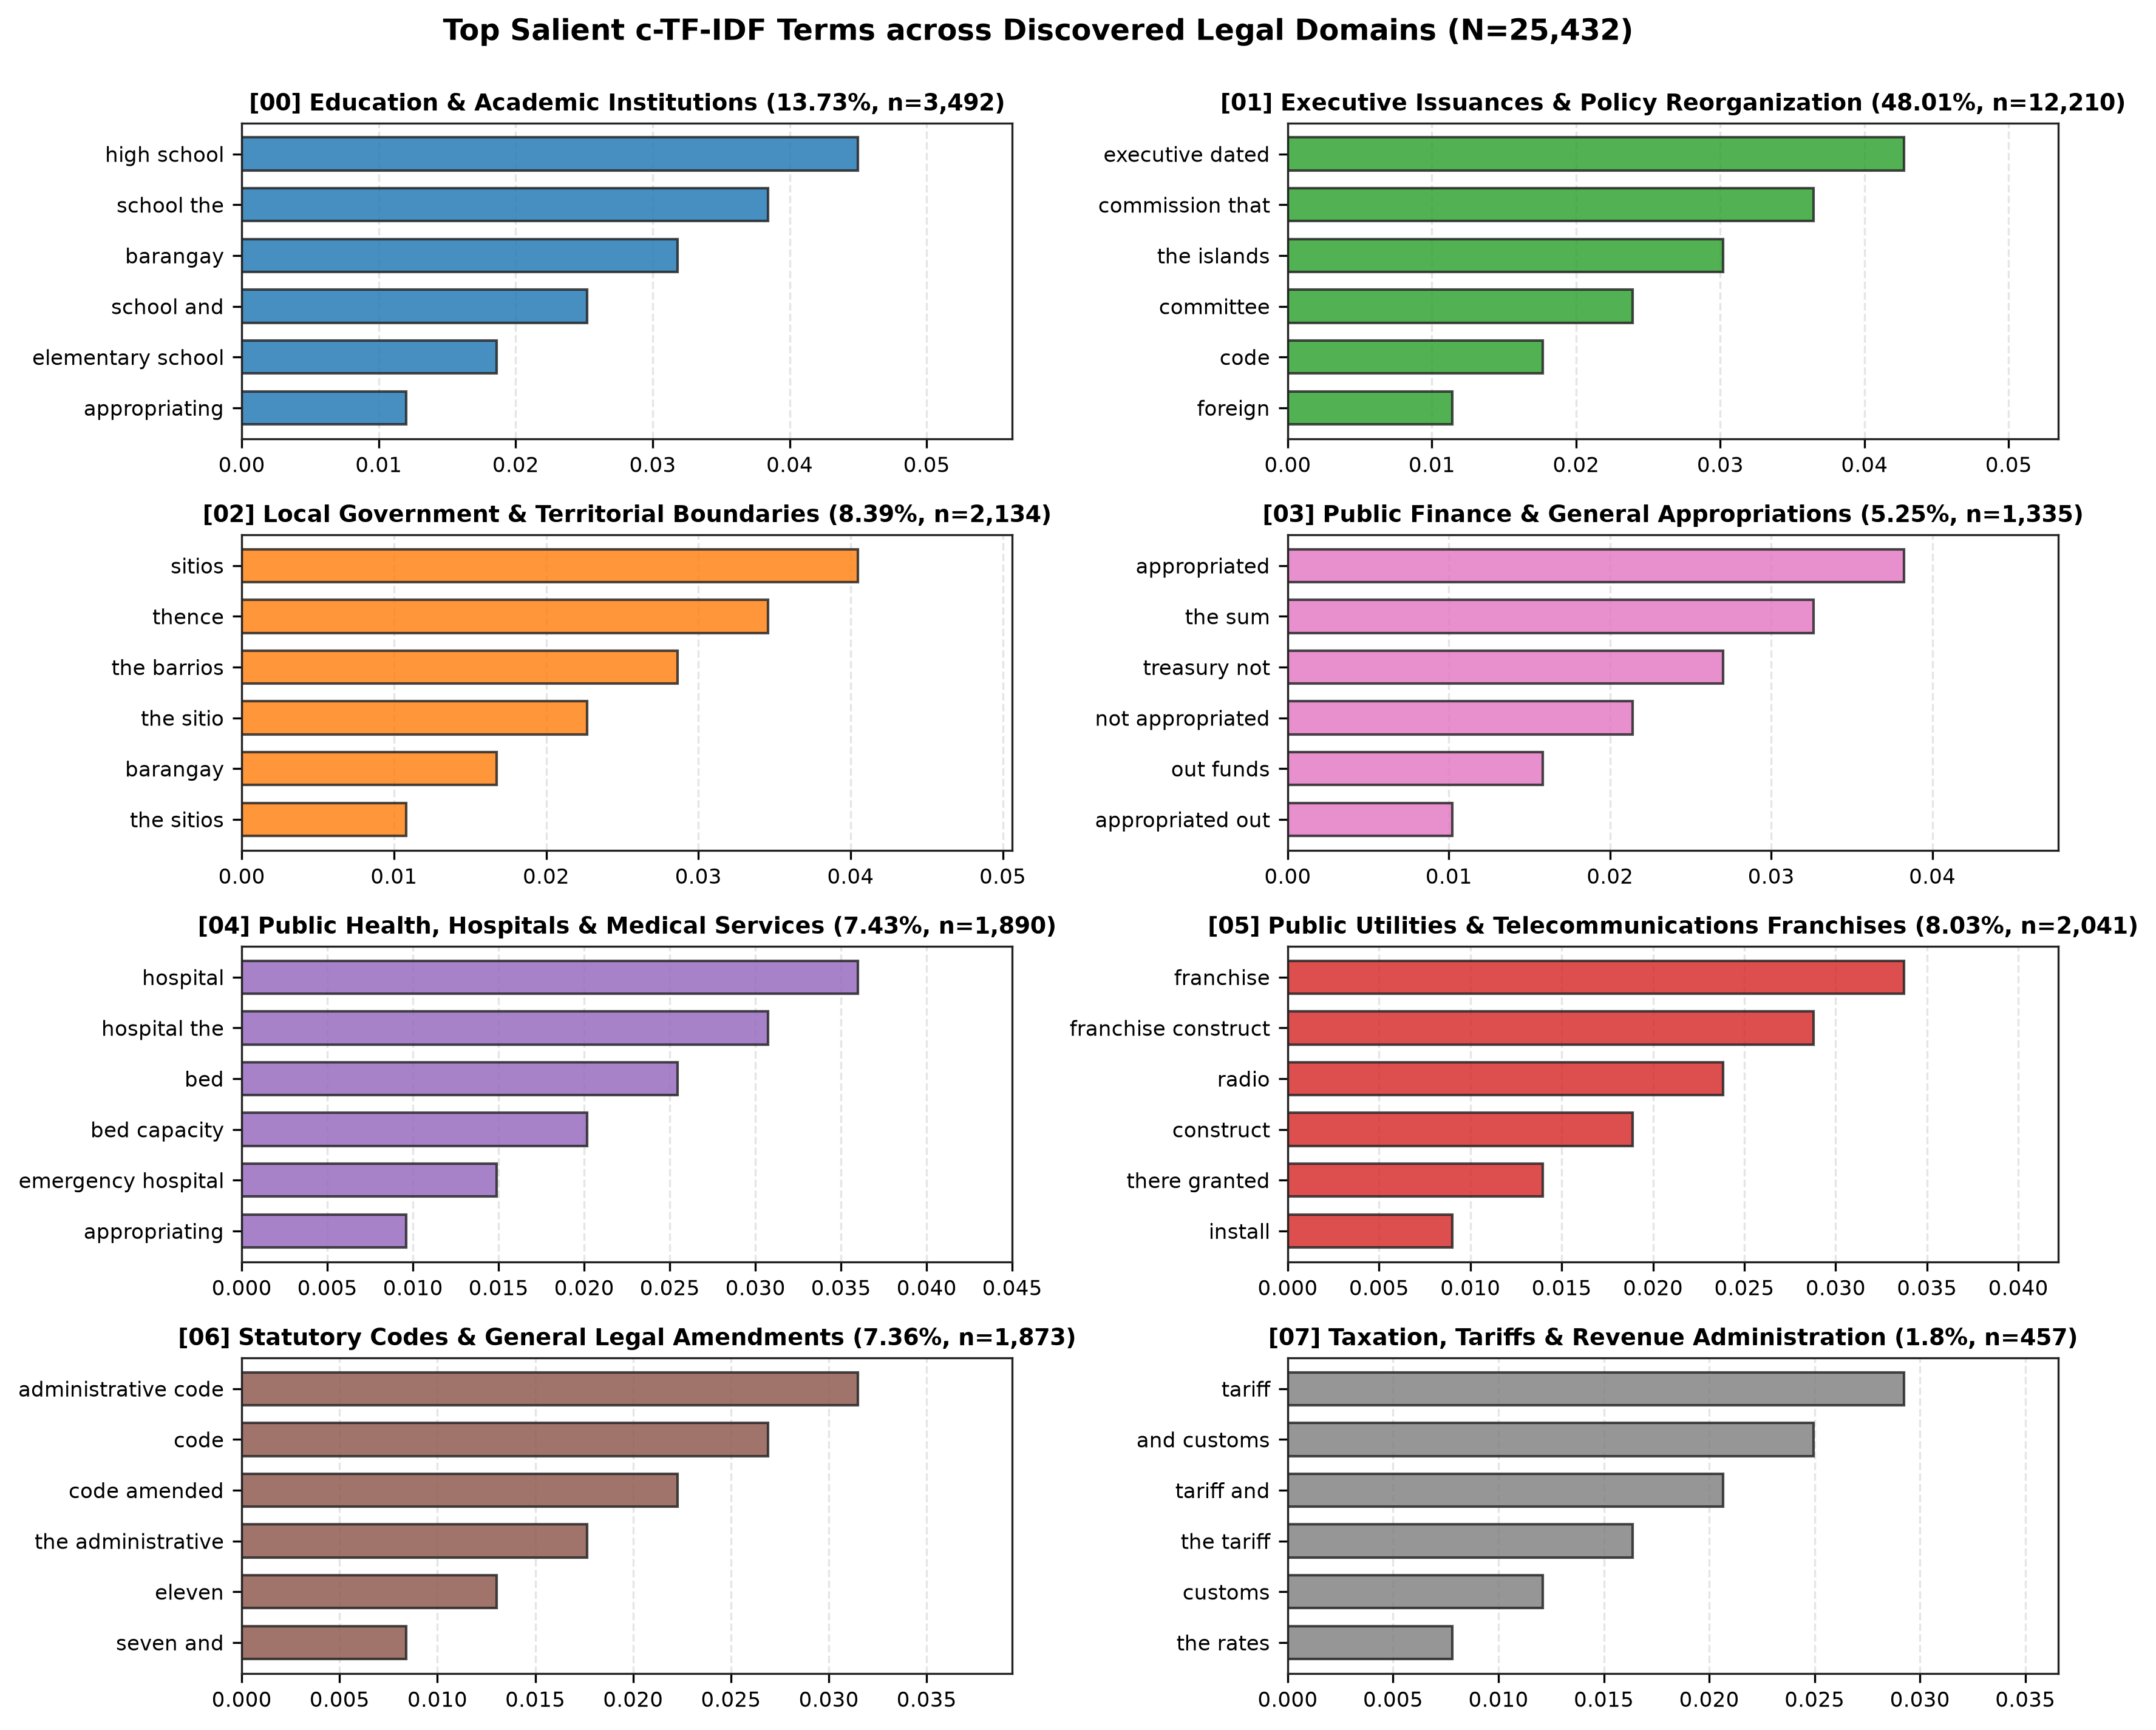
\includegraphics[width=0.78\linewidth]{figs/top_keywords_per_domain.png}
            \caption{Top Salient $c\text{-}TF\text{-}IDF$ Keyword Profiles across the Eight Consolidated Macro Legal Domains ($N = 25,432$).}
            \label{fig:top_keywords_per_domain}
        \end{figure}

        The vocabulary profiles confirm that each macro domain is defined by operative legal terminology unique to its statutory field. Specialized clusters such as public health are dominated by concrete institutional terms, including ``hospital,'' ``bed capacity,'' and ``medical center.'' Similarly, territorial boundary enactments display spatial cartographic markers such as ``sitio,'' ``barrio,'' and directional bearings. General administrative codes feature broader amendment verbs and statutory cross-references. These distinct vocabulary distributions confirm that the unsupervised clustering algorithm captures authentic legal subject matter across diverse legislative eras.

        To examine how individual lawmaking authorities contribute to these eight subject areas, the proponents mapped the six statutory instruments across the consolidated macro domains. In Philippine legislative history, different legal instruments serve distinct constitutional functions, ranging from broad congressional acts to presidential executive directives. Figure~\ref{fig:statute_source_domain_cross_allocation} presents this cross-allocation matrix, detailing both absolute enactment counts and percentage distributions for each statutory source. This cross-tabulation reveals an explicit division of legal responsibility across Philippine statutory instruments. Analyzing this allocation confirms that regulatory subjects concentrate within specific legislative formats rather than distributing evenly across the archive.

        \begin{figure}[!htbp]
            \centering
            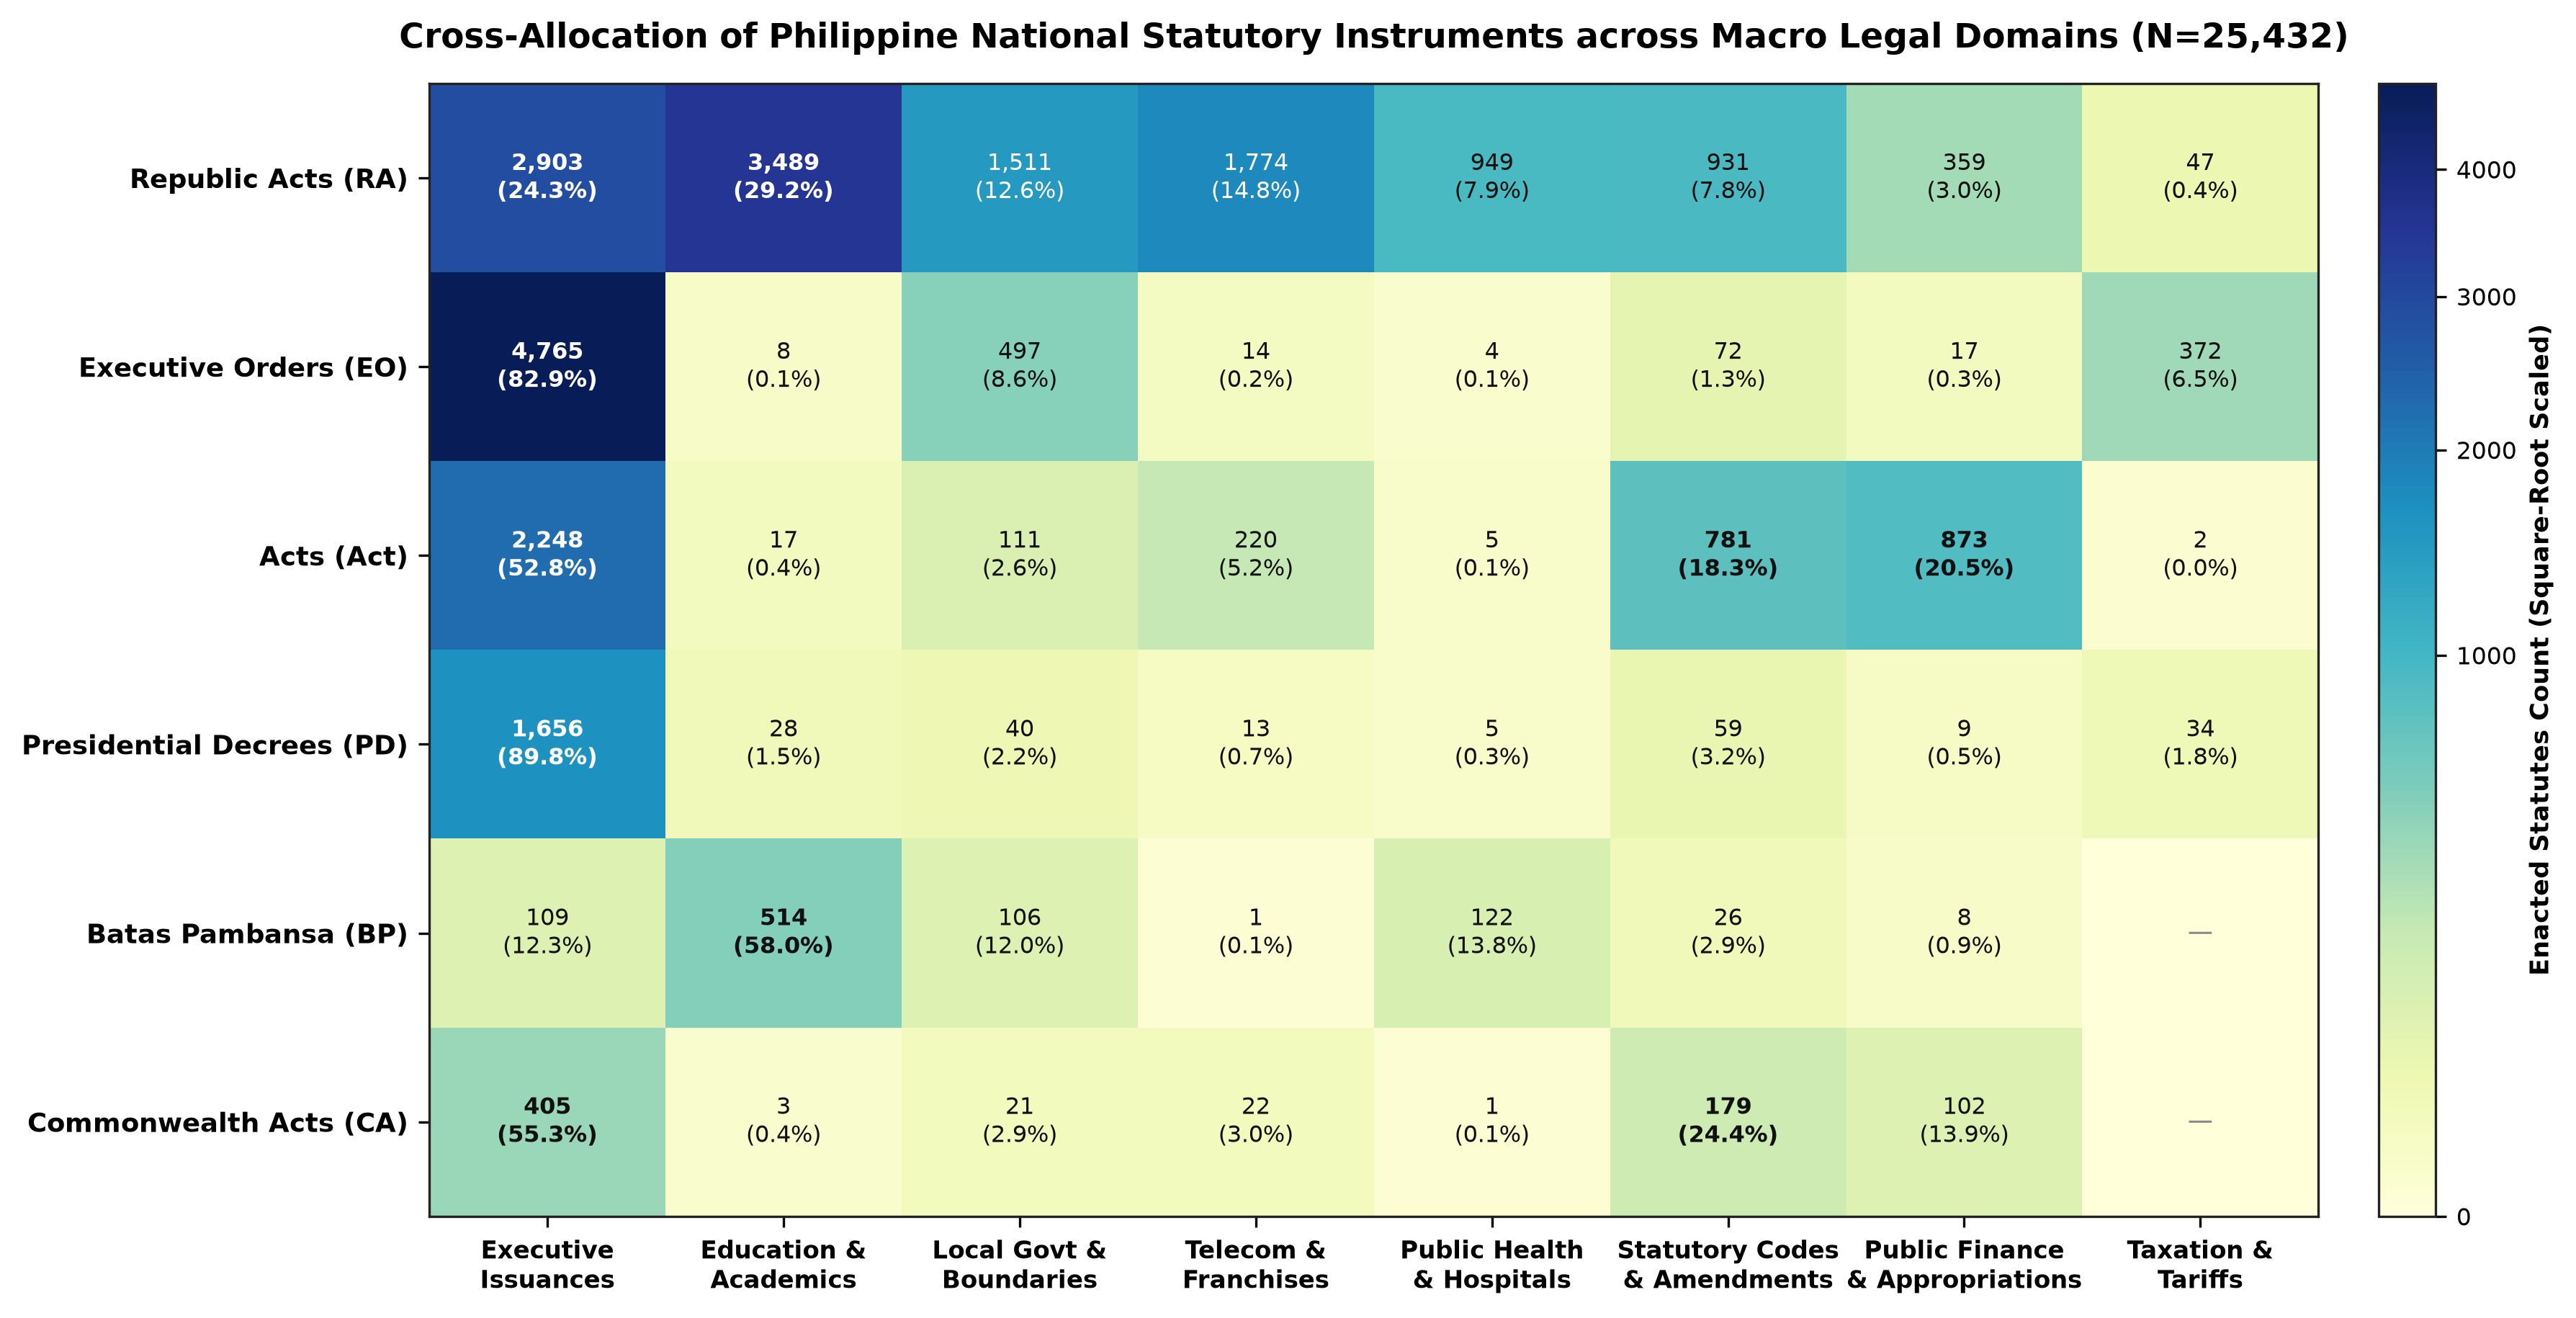
\includegraphics[width=0.80\linewidth]{figs/statute_source_domain_cross_allocation.png}
            \caption{Cross-Allocation Matrix of the Six National Statutory Instruments across the Eight Consolidated Macro Legal Domains ($N = 25,432$).}
            \label{fig:statute_source_domain_cross_allocation}
        \end{figure}

        The cross-allocation matrix reveals that congressional enactments and executive orders govern entirely separate legal spheres. Republic Acts account for nearly all specialized regulatory measures, containing 99.9\% of academic enactments and 86.9\% of telecommunications franchises. In contrast, Executive Orders concentrate heavily within administrative policy (82.9\%) and presidential tariff adjustments (81.4\%). Because municipal ordinances regulate local community behavior rather than internal executive operations, matching draft local clauses against executive orders produces high rates of irrelevant candidate retrievals. These empirical disparities validate using statutory source indicators and domain filters during Stage~1 retrieval to keep candidate shortlists focused on genuine regulatory mandates.

        To confirm that the topic pipeline discovered authentic legal boundaries rather than grouping surface vocabulary, the proponents evaluated the model using a stratified 80/20 train/test split. The 80/20 proportion follows the standard Pareto partition for large-scale legal collections exceeding 20,000 documents~\cite{aggarwal2012mining}, withholding 20\% of the corpus (5,087 statutes) to test generalizability on unseen enactments while training the model on the remaining 80\% (20,345 statutes). In statistical testing, an out-of-sample holdout of 5,087 legal texts provides high statistical power with a margin of error below $\pm 1.4\%$, making repetitive cross-validation computationally redundant as vocabulary frequencies and SVD components stabilize asymptotically at this volume. Stratified sampling preserves the natural historical proportions of the eight macro domains, ensuring that smaller regulatory categories like taxation (1.80\%, $N=457$) maintain adequate representation in the test set ($N_{\text{test}} \approx 91$) without class starvation. Table~\ref{tab:topic_holdout_validation} presents the out-of-sample performance scores, default random baselines, literature targets, and empirical verdicts across all evaluation criteria.

        \begin{table}[!htbp]
            \centering
            \footnotesize
            \renewcommand{\arraystretch}{0.95}
            \setlength{\tabcolsep}{3.5pt}
            \caption{Empirical Holdout Validation Metrics, Baseline Comparisons, and Literature Targets for the Topic Modeler ($N_{\text{train}} = 20,345, N_{\text{test}} = 5,087$)}
            \label{tab:topic_holdout_validation}
            \begin{tabularx}{\linewidth}{>{\RaggedRight}p{4.5cm}cc>{\Centering}p{2.3cm}>{\RaggedRight}X}
                \toprule
                \textbf{Validation Metric / Benchmark Test} & \textbf{Observed} & \shortstack[c]{\textbf{Default}\\\textbf{Baseline}} & \shortstack[c]{\textbf{Target}\\\textbf{Range}} & \textbf{Empirical Verdict} \\
                \midrule
                Out-of-Sample Supervised Accuracy & 97.37\% & 12.50\% & $\ge 85.0\%$ & Strong Generalization \\
                Out-of-Sample Macro F1-Score & 96.26\% & 12.50\% & $\ge 80.0\%$ & Balanced Discrimination \\
                Mean Test Cosine \mbox{Confidence} & 0.5508 & 0.1250 & $> 0.4000$ & Strong Dominant Probability \\
                High-Confidence Predictions ($\ge 0.50$) & 56.97\% & $< 20.0\%$ & $> 50.0\%$ & Clear Majority Cluster \\
                Holdout Cosine Silhouette Score & 0.1602 & $\le 0.0000$ & $0.1000\text{--}0.2000$ & Solid Text Separation \\
                Holdout Davies-Bouldin Index & 2.4496 & $> 4.0000$ & $2.0000\text{--}3.0000$ & Compact Cluster Scatter \\
                \midrule
                \multicolumn{5}{l}{\textbf{Explicit Statutory Title Probes} (\textit{Unambiguous Indicator Subsets, $N=1,259$})} \\
                \midrule
                Telecom Franchise Pattern & 97.8\% & 12.50\% & $> 90.0\%$ & High Precision ($N=360$) \\
                Hospital Bed Capacity \mbox{Pattern} & 96.6\% & 12.50\% & $> 90.0\%$ & High Precision ($N=203$) \\
                School Infrastructure \mbox{Pattern} & 92.2\% & 12.50\% & $> 90.0\%$ & High Precision ($N=645$) \\
                Judiciary \& Court Pattern & 72.5\% & 12.50\% & $> 70.0\%$ & Acceptable ($N=51$, embedded laws) \\
                \bottomrule
            \end{tabularx}
        \end{table}

        The supervised benchmark results confirm that the discovered macro domains generalize reliably to unseen legislation. In an eight-domain classification setting, the uniform proportional chance criterion established by Morrison~\cite{morrison1969interpretation} yields a default random baseline accuracy of only 12.50\% ($1/8$). In contrast, the validation classifier reached an out-of-sample accuracy of 97.37\% and a Macro F1-Score of 96.26\%, surpassing the 85.0\% target threshold typically expected for reliable document categorization~\cite{aggarwal2012mining}. To provide an external sanity check beyond learned cluster labels, the evaluation tested four explicit statutory title probes ($N=1,259$ total) where legislative intent is unmistakable from the statutory catchline. The model achieved 97.8\% precision on telecommunications franchises ($N=360$), 96.6\% on hospital bed capacity acts ($N=203$), and 92.2\% on school infrastructure laws ($N=645$). The lower precision on court reorganization acts (72.5\%, $N=51$) occurs because historical judicial reforms were frequently enacted as embedded chapters within general administrative codes rather than separate court charters.

        The probabilistic confidence metrics evaluate how decisively the model assigns unseen statutes to their respective legal domains. In an eight-domain distribution, equal uncertainty across all classes results in a default probability baseline of 0.1250 (12.50\%) under standard multinomial chance models~\cite{morrison1969interpretation}. Across all 5,087 holdout statutes, the model achieved a Mean Test Cosine Confidence of 0.5508 (55.08\%), exceeding the typical 0.4000 operational target and demonstrating that the top assigned category captured more than half of the total probability mass. Furthermore, 56.97\% of all unseen statutes were classified with high certainty ($\ge 0.50$ probability), well above the majority target threshold of 50.0\%. The remaining 43.03\% of statutes received confidence scores between 0.25 and 0.49 because Philippine legislation frequently addresses multiple regulatory areas within a single enactment. For example, general appropriations bills and administrative reorganizations distribute their probability across public infrastructure and local governance while still correctly assigning the dominant primary domain.

        The geometric clustering metrics evaluate whether the 64-dimensional SVD vector space forms well-separated and compact legal clusters. The holdout evaluation yielded a Cosine Silhouette Score of 0.1602 against the foundational baseline established by Rousseeuw~\cite{rousseeuw1987silhouettes}, where values near or below zero indicate overlapping, unseparated data points. While synthetic low-dimensional benchmarks often target silhouette scores above 0.50, text-mining literature demonstrates that high-dimensional document clustering rarely exceeds 0.20 due to shared vocabulary across legal topics~\cite{aggarwal2012mining}. In natural language processing, a positive silhouette score between 0.10 and 0.20 provides solid evidence of meaningful cluster cohesion and separation. Similarly, the model achieved a Davies-Bouldin Index of 2.4496, well within the target range of 2.0000 to 3.0000 formulated by Davies and Bouldin~\cite{davies1979cluster} and substantially below the diffuse clustering threshold of 4.0000. These geometric measurements prove that the topic model establishes stable, mathematically separated legal boundaries before documents are indexed for coarse retrieval.

        \subsubsection{Preprocessing and Chunking}
        To determine effective chunking boundaries, the proponents analyzed document and section lengths across the entire national statutory corpus ($N = 25,432$). Full national enactments span a wide spectrum of text lengths, ranging from brief presidential decrees to massive statutory codes containing hundreds of articles. In transformer-based natural language processing, text is segmented into subword units or ``tokens'' (where 1,000 tokens correspond to approximately 750 words in formal English legal text) and processed through self-attention mechanisms bounded by a fixed maximum sequence length (typically 512 tokens)~\cite{devlin2019bert}. Direct document-level matching causes severe context dilution because long enactments far exceed this 512-token sequence limit~\cite{wu2025aiir}. Dividing national legislation into natural section units aligns with legislative drafting structures where each section forms a self-contained legal rule. Figure~\ref{fig:statutory_length_disparity} illustrates the character length distribution of full statutes alongside the empirical token distributions and domain compliance rates across all 164,620 extracted section provisions.

        \begin{figure}[htbp]
            \centering
            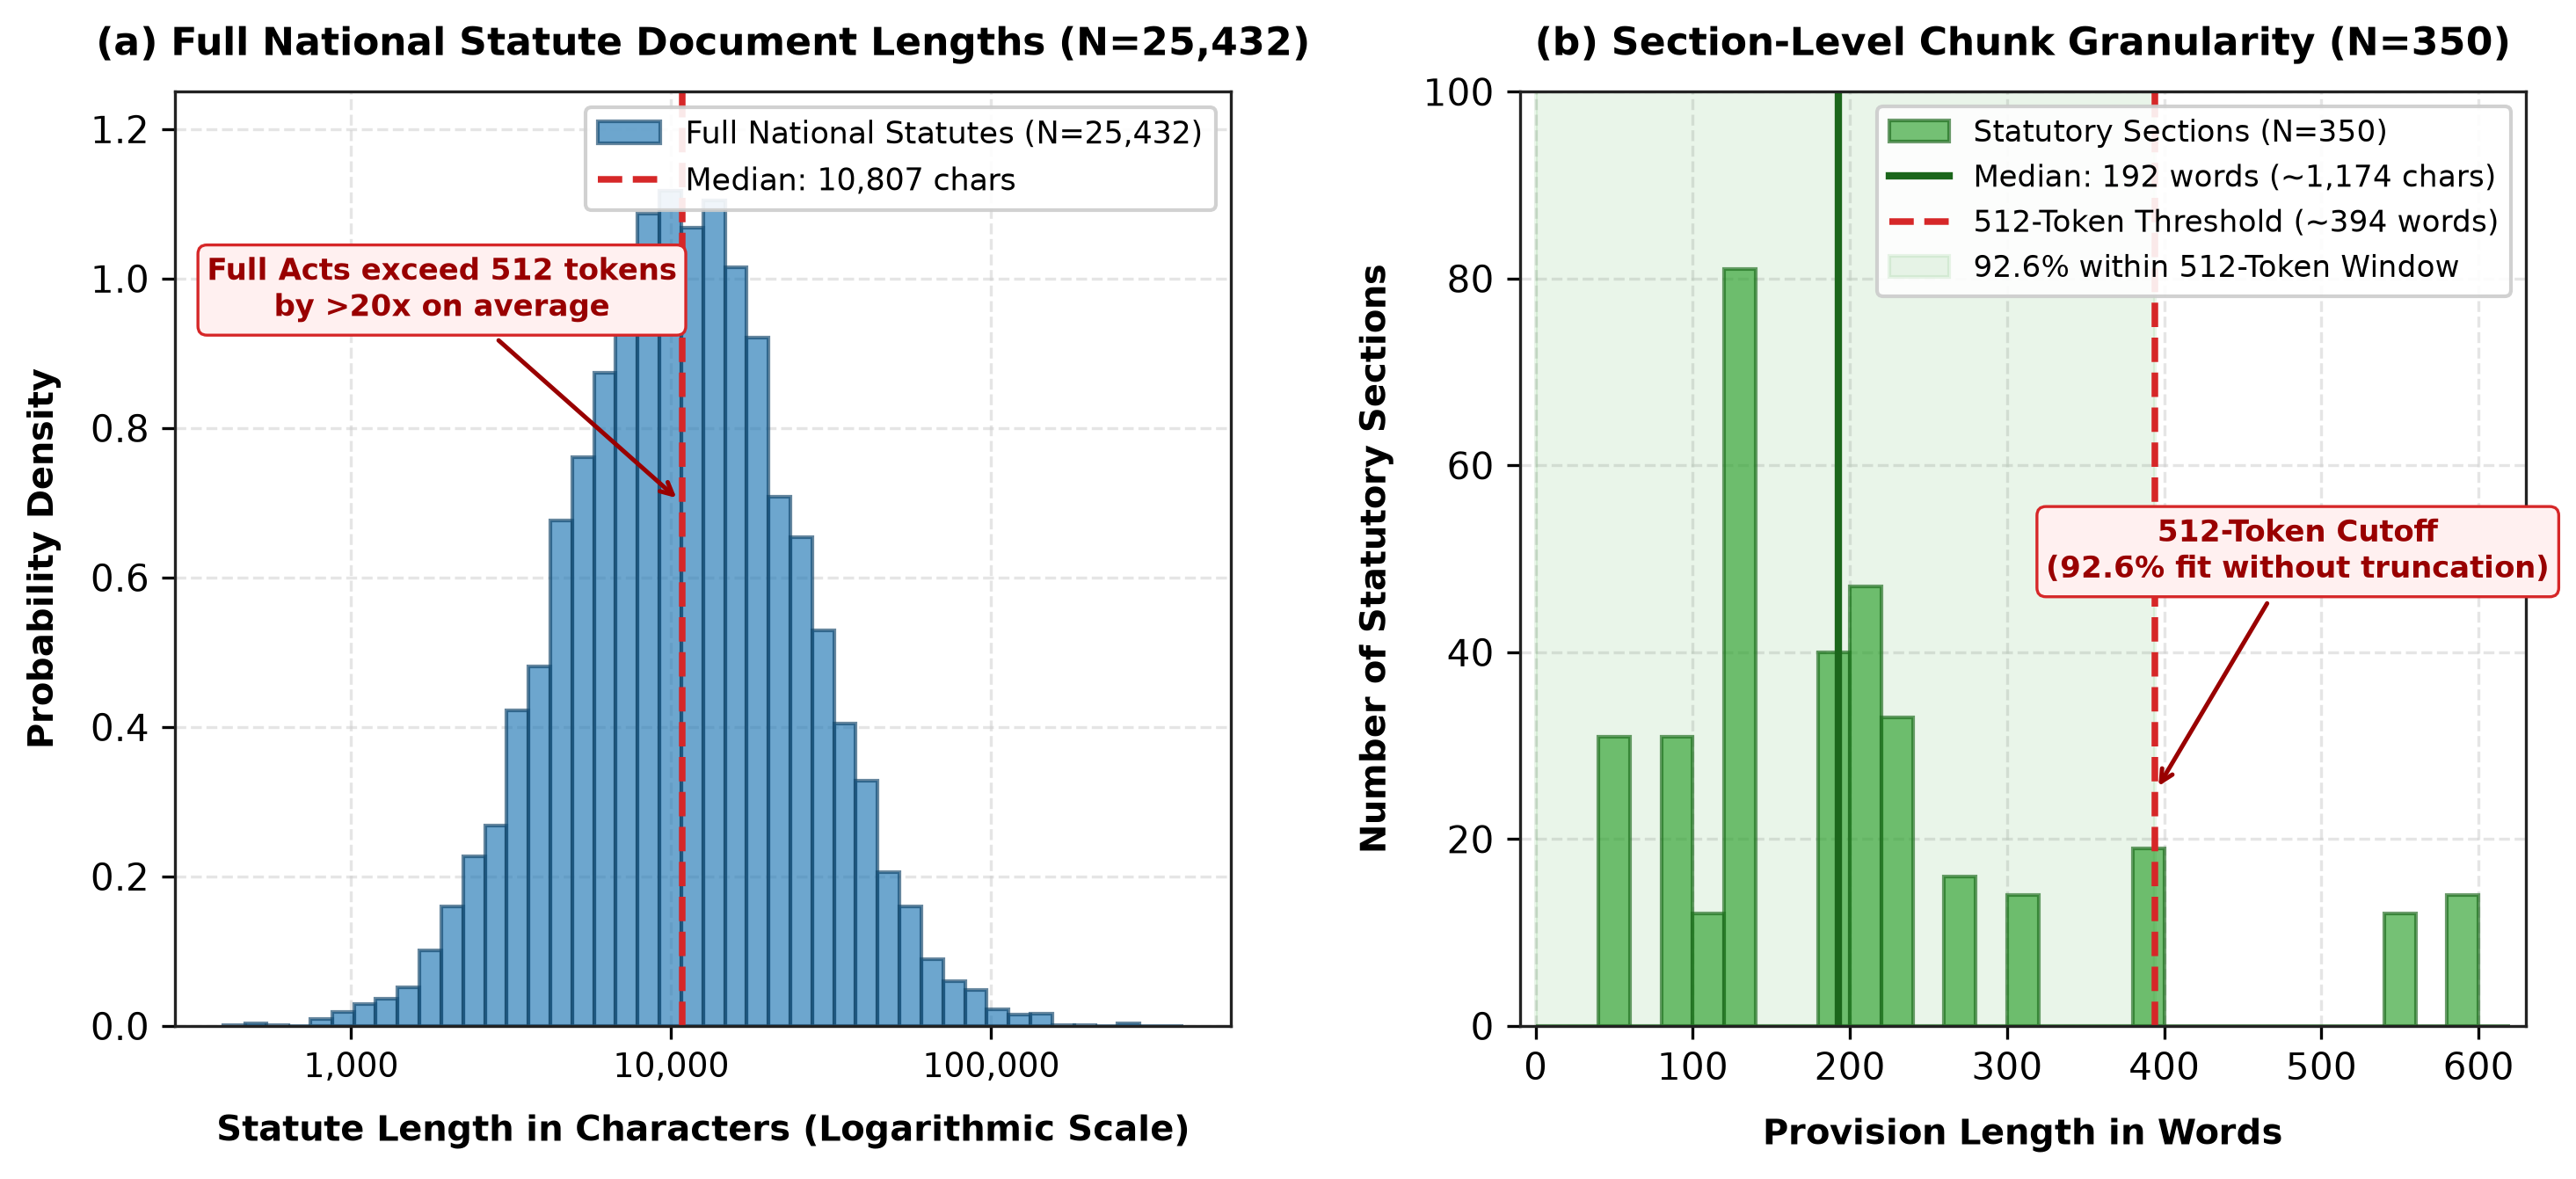
\includegraphics[width=0.98\linewidth]{figs/statutory_length_disparity.png}
            \caption{Document Length Distributions, Prepended Section Token Granularity, and 512-Token Compliance Rates across the Philippine National Statutory Corpus ($N = 25,432$ Statutes, $N = 164,620$ Sections).}
            \label{fig:statutory_length_disparity}
        \end{figure}

        The empirical distributions confirm that section-level chunking provides a practical input format for statutory retrieval. Across all 25,432 national statutes, full enactments exhibit a median length of 10,807 characters, with comprehensive codifications regularly exceeding one hundred thousand characters. In contrast, an empirical census of all 164,620 statutory sections reveals a median length of only 122.0 tokens after prepending the structural metadata header. Exactly 94.83\% of all prepended provisions (156,109 sections) fit completely within the 512-token attention window of standard transformer encoders. Segmenting legislation at natural section boundaries preserves complete legal rules while eliminating the need for arbitrary sliding windows that fragment statutory conditions.

        Examining token lengths across the eight macro legal domains explains how drafting styles differ between statutory subjects. Regulatory categories interact closely with municipal powers and demonstrate high compliance rates, led by Public Health (99.16\%), Public Utilities (98.78\%), Education (98.64\%), and Taxation (95.86\%). The only category with a noticeable exceedance tail is Local Government and Territorial Boundaries, where 12.54\% of sections exceed 512 tokens due to lengthy metes-and-bounds surveying descriptions. Across the entire national corpus, only 5.17\% of provisions exceed the 512-token threshold.

        To handle provisions in this 5.17\% tail without information loss under standard-context models, the pipeline implements a hierarchical overlapping sub-chunking fallback. Adapting the sliding window strategy formulated by Devlin et al.~\cite{devlin2019bert} for transformer sequence constraints, when an extracted statutory section exceeds a safety threshold of 448 tokens, the preprocessing module divides the section into overlapping sub-chunks using a window of $w = 384$ tokens and a stride of $s = 256$ tokens (128-token overlap). Capping the sub-chunk window at 384 tokens reserves a 64-token structural buffer within the 512-token ceiling to accommodate the prepended metadata header along with mandatory special tokens ($[CLS]$, $[SEP]$)~\cite{devlin2019bert}. Each sub-chunk preserves the prepended structural metadata header $\left[ \text{Statute Title}, \text{ Section } S_i\text{: Catchline} \right]$ to maintain institutional context. In Stage~1 retrieval, the parent provision embedding is computed by mean-pooling the sub-chunk vectors, capturing semantic concepts across all paragraphs. In Stage~2 inference, the Cross-Encoder evaluates each sub-chunk independently against the local ordinance hypothesis $h$, determining the provision-level conflict through max-pooling across sub-chunk contradiction probabilities:
        \[
            \hat{P}(\text{Contradiction} \mid p_i, h) = \max_{j} P\left(\text{Contradiction} \mid p_{i,j}, h\right)
        \]
        where $p_{i,j}$ denotes the $j$-th sub-chunk of statutory section $p_i$. This max-pooling aggregation ensures that an isolated prohibition or restrictive condition buried deep in a multi-paragraph section triggers the contradiction alert without being diluted by surrounding agreeable text.

        Alongside the sub-chunking fallback, the proponents evaluate ModernBERT as a long-context candidate architecture~\cite{warner2024modernbert, kadowaki2025modernbert}. By combining FlashAttention-2 with rotary positional embeddings, ModernBERT natively processes input sequences up to 8,192 tokens, completely bypassing the need for text segmentation. The researchers hypothesize that ModernBERT is uniquely valuable for this 5.17\% tail of lengthy codifications and boundary descriptions where sequence truncation could otherwise occur. However, for the 94.83\% majority of concise provisions with a median length of only 122 tokens, standard-context architectures such as DeBERTa-v3~\cite{he2023debertav3} and MiniLM~\cite{reimers2019sentencebert} may achieve sharper semantic discrimination and faster inference on local office workstations. Evaluating both model families directly tests whether native long-context support outperforms compact, standard-window models across Philippine statutory texts.

        After establishing the need for granular text units, the preprocessing pipeline cleans local ordinance texts and national statutory provisions. Custom regular expressions find and remove repetitive introductory preamble paragraphs and official signature blocks from city ordinances. Unlike ordinary documents, legal acts follow an organized structure divided into numbered chapters and sections. The researchers divide statutes at the section level rather than using fixed word-count windows~\cite{wu2025aiir}. In Philippine legal drafting, each section acts as a complete rule, stating a main legal command along with its specific conditions and exceptions.

        Splitting text by an arbitrary word count can easily cut a legal rule in half, separating exceptions from the main requirement. When sub-clauses are separated this way, they lose the context of who must follow or enforce the rule. To preserve complete legal meaning, the preprocessing pipeline adds a structural metadata header to each chunk before saving it in the vector database. Every extracted statutory section begins with a header containing the statute title, section number, and section title:
        \[
            \mathbf{x}_{\text{chunk}} = \left[ \text{Statute Title}, \text{ Section } S_i\text{: Catchline} \right] \mathbin{\Vert} \mathbf{t}_{\text{verbatim}}
        \]
        where $\mathbf{t}_{\text{verbatim}}$ denotes the exact text extracted from Lawphil, and $\mathbin{\Vert}$ represents text joining. This prefix helps the Stage~2 Cross-Encoder immediately recognize the governing authority and official context of the provision.

        The practical need for these headers is shown by sections within composite legal codes. In Republic Act No.~7160, Section~447 sets penalty limits for municipalities, while Section~458 sets distinct penalty limits for city councils. Without adding the section title and number, downstream Cross-Encoders can confuse different levels of local government and misjudge municipal powers. Adding the structural metadata ensures that the model evaluates each legal clause under its correct administrative level. As a result, the vector embeddings retain both the exact wording of the clause and its broader statutory context.

        \subsubsection{Exception Handling}
        A key challenge in conflict detection is telling the difference between a real legal clash and an authorized legal exception. In regulatory laws, general prohibitions and permitted exceptions often appear in the same section using conditional phrasing. Because statutory sections average between 200 and 500 words, an entire section fits within the 512-token input limit of candidate Cross-Encoders. The model's attention mechanism can read the general rule and its internal exceptions together, preventing the system from incorrectly flagging valid local exceptions as conflicts. This structure helps keep the legal relationship between general rules and local exceptions clear.

        When a general ban and an exception appear in separate sections of a statute, the pipeline relies on the two-stage search process. An ordinance clause that drafts an authorized exception often uses words that match both the general ban and the exception section. The Stage~1 hybrid retriever searches both keyword and vector indexes, helping bring both candidate sections into the top-$k$ candidate shortlist. Stage~2 then evaluates each candidate section individually, allowing the system to identify the authorizing provision and confirm that the local rule is valid. This multiple-candidate review prevents premature conflict warnings on complex laws that place their exceptions in separate sections.

        In Philippine statutory construction, related enactments and provisions governing the same subject matter must be interpreted together as a harmonious whole under the doctrine of \textit{in pari materia}~\cite{agpalo2009statutory}. Under this established legal rule, an isolated subsection cannot be understood in a vacuum without the overarching context of its governing section and related statutory exemptions. If an ordinance draft relies on an authorized statutory exemption, evaluating a specific clause like a penalty rule without retrieving the parent exception can trigger an incorrect conflict warning. The system addresses this challenge by prepending hierarchical catchlines to granular sub-clauses during preprocessing and using hybrid retrieval to pull both general bans and specific exception clauses into the candidate shortlist. The Cross-Encoder can then evaluate the draft against the authorizing exception clause and assign an Entailment classification, confirming that the local measure operates within valid legislative authority.

        \subsection{Ground Truth Benchmark Construction}
Evaluating candidate Cross-Encoder models in Stage~2 requires a high-quality ground truth dataset. Unlike the broad search phase, the Natural Language Inference (NLI) model needs expert-verified examples to train and measure its classification accuracy. Because standard NLP benchmarks do not include Philippine local laws, a custom dataset had to be created for Davao City. This curated collection provides a clear benchmark for identifying legal conflicts between draft local ordinances and national statutes. In this way, the ground truth dataset connects basic language processing with real-world legal analysis.

\subsubsection{Span Pairing}
        \label{sec:span_pairing}
        To construct a representative ground truth benchmark, candidate statutory premises must reflect the full breadth of Philippine national law. During the exploratory phase of this research, the proponents conducted preliminary machine learning experiments on the national statutes, uncovering severe class imbalances and repetitive drafting formulas across historical eras. These exploratory findings directly informed the consolidated topic modeling architecture detailed in Section~\ref{sec:domain_categorization}, which organizes the corpus into eight validated Macro Legal Domains such as local governance, public health, and taxation. The proponents then sampled national statutory sections across these eight domains to establish the fixed premises for the evaluation benchmark. To evaluate multi-sentence legal commands without breaking internal qualifications, the pipeline uses Asymmetric Span-Level Pairing, coupling each statutory premise with a multi-sentence ordinance hypothesis block~\cite{yin2021docnli}. This asymmetric structure ($1\text{ premise vs } N\text{ hypothesis sentences}$) ensures that local exceptions, cross-references, and penalty conditions are evaluated together against the national law~\cite{koreeda2021contract}.

        To make the evaluation as realistic as possible, the drafted test sentences closely mirror the writing style of Davao City ordinances. The proponents analyzed municipal laws enacted between 2021 and 2025 to identify standard drafting phrases, administrative office names, and structural penalty clauses following the official drafting conventions of the Department of the Interior and Local Government (DILG)~\cite{dilg2022drafting}. Each drafted clause uses standard enacting syntax, such as: ``\textit{SECTION X. [TITLE]. --- It shall be unlawful for any person, natural or juridical, within the territorial jurisdiction of Davao City, to...}'' The draft sentences also name real local enforcement bodies, such as the City Transport and Traffic Management Office (CTTMO), the City Health Office (CHO), the City Environment and Natural Resources Office (CENRO), and the Business Bureau of Davao City. Operational units such as the Anti-Vices Task Force (AVTF) and the Davao City Police Office (DCPO) are also included to reflect genuine local enforcement.

        The synthetic ordinance clauses are also linked to real administrative districts in Davao City. Draft rules specify geographic areas from urban centers like Poblacion and Talomo to suburban districts like Buhangin and Toril. Local offices such as the City Disaster Risk Reduction and Management Office (CDRRMO) and the City Social Welfare and Development Office (CSWDO) are included to match actual city administration. This realistic drafting prevents evaluators from reviewing artificial example sentences that differ from real legal texts. As a result, the 15 Sangguniang Panlungsod legal researchers evaluate draft provisions that look like real measures introduced on First Reading.

        The proponents deliberately utilized expert-curated, domain-grounded hypothesis construction based on authentic local templates rather than unconstrained synthetic generation via large language models. Recent evaluations by Gururangan et al.~\cite{gururangan2018annotation} and Poliak et al.~\cite{poliak2018hypothesis} demonstrated that automated or crowd-generated NLI hypotheses frequently introduce severe ``annotation artifacts''—systematic lexical cues such as negation markers (``not'', ``never'') that allow neural models to cheat and predict contradictions without genuinely reading the statutory premise. In specialized legal domains, authoritative benchmarks such as SARA (tax law)~\cite{holzenberger2020a}, DocNLI~\cite{yin2021docnli}, and Clash-of-Leges~\cite{italiani2026clash} establish that rigorous evaluation requires domain-grounded hypotheses reflecting authentic legislative syntax, ensuring models are tested on genuine statutory reasoning rather than superficial generation heuristics.

        While the system uses multi-sentence spans to understand local context, it does not attempt cross-document multi-hop reasoning (detecting conflicts that appear only by combining two or more separate national laws). Resolving dependencies across multiple separate laws is an active research challenge in natural language inference. Current systems that attempt this require either complex knowledge graphs~\cite{lu2023multi} or very large generative language models~\cite{shen2025hopweaver}. Running those multi-premise models would exceed the consumer-grade hardware limits set for local government deployment. For this reason, the ground truth benchmark and the inference system focus strictly on single-premise evaluations.

        \subsubsection{Class Balancing and Adversarial Injection}
        In standard machine learning on tabular data, researchers often handle uneven classes using methods like the Synthetic Minority Over-sampling Technique (SMOTE)~\cite{chawla2002smote}. However, the proponents avoid continuous vector oversampling for this legal text pipeline. SMOTE creates artificial examples by interpolating between numerical feature vectors ($x_{\text{new}} = x_i + \lambda(x_{zi} - x_i)$). In high-dimensional language models representing discrete words, averaging or blending token vectors creates artificial representations that confuse attention layers and carry no real legal meaning. Simple word replacement also fails with legal texts because statutory words have exact legal definitions; for example, swapping mandatory words like ``shall'' with permissive words like ``may'' fundamentally changes a legal duty.

        To build a balanced, reliable Ground Truth dataset, the researchers combined historical legal records with expert-guided text adjustments. First, the researchers gathered documented legal clashes from local government records, including mayoral veto messages, repealed ordinances, and explicit statutory amendments~\cite{italiani2026clash}. Second, following the evaluation methods of Koreeda and Manning~\cite{koreeda2021contract} and Nie et al.~\cite{nie2020anli}, legal annotators introduced conflicting rules into real statutory provisions. Annotators reversed permissions, changed numerical zoning limits, and added conflicting penalties into ordinance clauses. This expert-guided process produced a balanced distribution across the Entailment, Neutral, and Contradiction classes in the 350 Ground Truth pairs, preventing class imbalance without creating unnatural legal phrasing.

    \subsubsection{Jurisprudential Difficulty Tiers}
        Building an effective evaluation benchmark requires pairs with varying levels of difficulty. If all contradiction examples were simple penalty ceiling violations or obvious word swaps, models could score well by memorizing shallow keyword patterns~\cite{mccoy2019right}. To construct a rigorous evaluation suite, the proponents adapted the difficulty tiering methodology established by Koreeda and Manning in the ContractNLI benchmark~\cite{koreeda2021contract}. This approach is supported by the behavioral stress-testing frameworks of Ribeiro et al.~\cite{ribeiro2020beyond} and Naik et al.~\cite{naik2018stress}, which separate surface competence tests from semantic challenge sets. Furthermore, the 30\% Tier~1, 40\% Tier~2, and 30\% Tier~3 quota follows the adversarial challenge partitioning established in benchmark engineering literature, such as SQuAD~2.0~\cite{rajpurkar2018know}, FEVER~\cite{thorne2018fever}, and ANLI~\cite{nie2020anli}. These foundational benchmarks establish that maintaining an adversarial challenge quota of 30\% to 40\% is optimal to prevent models from exploiting superficial lexical artifacts while preserving sufficient representation of standard rule-based compliance. Table~\ref{tab:conflict_difficulty_tiers} outlines the stratified difficulty tiers, legal conflict mechanisms, and representative examples for the 350-pair benchmark.

        \begin{table}[htbp]
            \centering
            \footnotesize
            \setlength{\tabcolsep}{4pt}
            \caption{Stratified Jurisprudential Difficulty Tiers for the 350-Pair Ground Truth Evaluation Benchmark}
            \label{tab:conflict_difficulty_tiers}
            \begin{tabularx}{\linewidth}{>{\RaggedRight}p{3.4cm}>{\centering\arraybackslash}p{1.4cm}>{\RaggedRight}X>{\RaggedRight}p{4.5cm}}
                \toprule
                \textbf{Difficulty Tier} & \textbf{Target Share} & \textbf{Legal Conflict Mechanism} & \textbf{Representative Statutory Example} \\
                \midrule
                \textbf{Tier 1: Surface \& Quantitative} & 30\% & Direct penalty ceiling violations and explicit changes in mandatory words (\textit{shall} converted to \textit{may}). & Local draft imposes a PHP~15,000 fine for traffic obstruction when RA 7160 Sec. 458 caps city penalties at PHP~5,000. \\
                \addlinespace[3pt]
                \textbf{Tier 2: Preemption \& Carve-Outs} & 40\% & Exceeding local regulatory powers under \textit{Magtajas}, and blanket local bans that omit statutory exceptions. & Draft ordinance enacts a total ban on commercial freight transit without exempting national agricultural and medical logistics. \\
                \addlinespace[3pt]
                \textbf{Tier 3: Latent \& Paraphrastic} & 30\% & Subtle conflicts where the draft redefines statutory terms or creates incompatible rules without using the exact statutory words. & Draft anti-vagrancy ordinance assigns apprehended minors to detention cells, violating non-custodial diversion under RA 9344 without citing the law. \\
                \bottomrule
            \end{tabularx}
        \end{table}

        The three difficulty tiers map directly to established Philippine municipal preemption doctrines and linguistic challenge categories, reflecting the jurisprudential distinction between rule-based and value-based normative conflicts formulated by Sartor~\cite{sartor2005legal} and Bench-Capon and Sartor~\cite{benchcapon2003theory}. Tier~1 evaluates surface and quantitative preemption, reflecting direct penalty ceiling violations under Section~458 of Republic Act No.~7160 and explicit modal verb clashes (\textit{shall} versus \textit{may}). Tier~2 adapts the ``negation by exception'' category from Koreeda and Manning~\cite{koreeda2021contract}, evaluating unhonored statutory exemptions and local overreach under \textit{Magtajas v. Pryce Properties}~\cite{scp1994magtajasvpryce} and \textit{City of Manila v. Laguio, Jr.}~\cite{scp2005manilavlaguio}. Tier~3 evaluates latent and paraphrastic contradictions, testing whether the model detects substantive statutory friction when a draft redefines terms without sharing exact statutory words. Allocating the benchmark into 30\% Tier~1, 40\% Tier~2, and 30\% Tier~3 establishes an adversarial quota that reflects real-world committee reviews while preventing models from exploiting simple lexical heuristics~\cite{mccoy2019right}.

        Grounding Tier~3 contradictions in legal doctrine ensures that models are evaluated on genuine language understanding rather than keyword presence. Under established Supreme Court rulings, a local council cannot enact indirect prohibitions that take away rights protected by national statutes~\cite{scp1994magtajasvpryce, scp2005manilavlaguio}. To enforce this distinction during testing, the proponents verified that all 104 Tier~3 draft sentences contain zero numbers or monetary amounts. Without explicit numerical clues, the Cross-Encoder must evaluate the underlying legal meaning of the text, such as recognizing when an anti-vagrancy draft detains minors in violation of Republic Act No.~9344. This design ensures that the benchmark provides an authentic diagnostic test of semantic preemption for the subsequent analysis in Chapter~4.

        \subsubsection{Annotation Workflow}
        Classifying the sampled text pairs requires domain-specific legal training to ensure authentic and reliable labels. The Davao City Sangguniang Panlungsod currently comprises 24 elected councilors across the city's three legislative districts, supported by a professional staff of approximately 48 active legal researchers~\cite{cortez2025leadership}. In the initial administrative correspondence transmitted to the Sangguniang Panlungsod Secretariat alongside the Legal Annotation Guidebook, the proponents formally requested a cohort of 15 volunteer legal researchers. Unlike general NLP tasks that rely on open crowdsourcing, legal natural language inference requires formal statutory interpretation skills to prevent superficial keyword matching~\cite{snow2008cheap, zheng2021when}. The recruited legal researchers review local ordinances as their regular professional duty, providing the necessary institutional competence for building a dependable gold standard~\cite{chalkidis2022lexglue}.

        To establish an objective and transparent panel structure, the proponents gathered baseline qualifications during the initial intake communication. The intake request systematically recorded two key criteria from each volunteer: highest educational attainment and total years of professional experience in legislative drafting. Using these reported credentials, the 15 researchers were organized into five balanced sub-panels of three members each ($k = 3$). Within each three-member sub-panel, the evaluator possessing the highest educational attainment and the longest drafting tenure was designated as that panel's Senior Annotator. The proponents then communicated these panel assignments and Senior Annotator designations in a follow-up confirmation email to establish operational readiness before annotation began.

        Following the consensus guidelines adapted from Ablazo~\cite{ablazo2019designing}, a label is accepted into the final Ground Truth if at least two of the three reviewers in a sub-panel agree. In cases where all three reviewers select different categories, resulting in a three-way split with no majority, the pair is referred to that panel's designated Senior Annotator for binding qualitative adjudication~\cite{gao2022hierarchical, artstein2008inter}. The Senior Annotator reviews the pair against the standardized codebook to resolve whether the split arose from statutory ambiguity or an overlooked proviso. This hierarchical adjudication step ensures that every item in the 350-pair benchmark reaches an authoritative label while preserving the initial independent ratings for calculating Fleiss' Kappa ($\kappa$). Maintaining this structured division between initial independent scoring and expert tie-breaking guarantees both statistical validity and qualitative consistency across the dataset.

        \subsubsection{Annotation Codebook}
        To help the 15 legal researchers apply consistent criteria, the proponents developed a standardized Legal Annotation Codebook. Adapting principles from Koreeda and Manning~\cite{koreeda2021contract} and Italiani et al.~\cite{italiani2026clash}, the codebook turns the three-class NLI framework into clear legal decision rules. Each evaluated pair consists of a single national statute section as the premise and a multi-sentence municipal ordinance clause as the hypothesis. Annotators assign one of three labels: Contradiction, Entailment, or Neutral. Table~\ref{tab:annotation_codebook} summarizes the working definitions, legal triggers, and example patterns used in the annotation guidelines.

        \begin{table}[htbp]
            \centering
            \footnotesize
            \setlength{\tabcolsep}{4pt}
            \caption{Sangguniang Panlungsod Ground Truth Legal Annotation Codebook and Decision Rules}
            \label{tab:annotation_codebook}
            \begin{tabularx}{\linewidth}{>{\RaggedRight\arraybackslash}p{2.4cm}>{\RaggedRight\arraybackslash}p{4.0cm}>{\RaggedRight\arraybackslash}X>{\RaggedRight\arraybackslash}p{4.0cm}}
                \toprule
                \textbf{Logical State} & \textbf{Operational Legal Definition} & \textbf{Primary Legal and Structural Triggers} & \textbf{Representative Statutory Pattern} \\
                \midrule
                \textbf{Contradiction} & The municipal ordinance prohibits what national statute permits, permits what statute prohibits, or exceeds statutory ceilings~\cite{scp1994magtajasvpryce}. & Clashes in mandatory words (\textit{shall} vs. \textit{may}); penalty limit violations (RA 7160 Sec. 458); territorial or franchise preemption. & National statute caps ordinance fines at PHP~5,000; draft ordinance mandates a PHP~15,000 penalty. \\
                \addlinespace[3pt]
                \textbf{Entailment} & The municipal ordinance directly executes, complies with, or derives its regulatory authority from the national premise without adding conflicting mandates. & Compliant devolved implementation; literal statutory adoption; regulatory enforcement within prescribed legislative boundaries. & Local draft establishes a municipal health board strictly adhering to the composition mandated by RA 7160. \\
                \addlinespace[3pt]
                \textbf{Neutral} & The national statute and municipal ordinance address the same broad legal domain, but govern independent obligations without mutual conflict or derivation. & Shared topic without direct legal clash; complementary administrative scopes; distinct non-overlapping legal subjects. & National statute establishes hospital licensing standards; local draft regulates municipal market sanitary permits. \\
                \bottomrule
            \end{tabularx}
        \end{table}

        The decision rules for Contradiction directly apply the consistency test established in the Magtajas Doctrine~\cite{scp1994magtajasvpryce}. Because local governments have delegated rather than unlimited legislative powers under Republic Act No.~7160~\cite{philgov1991ra7160}, any local draft that exceeds national statutory limits is legally invalid (*ultra vires*). Annotators look for shifts in mandatory language, such as turning a strict command (``shall'') into an optional choice (``may''), or removing an exemption that national law protects. In the test samples, numerical rules are audited against national limits, including tax caps and penalty ceilings. These criteria ensure that conflict warnings highlight actual legal problems rather than minor wording choices.

        The guidelines follow a structured consensus process to resolve disagreements among the three panel reviewers. When two or three reviewers agree, the majority label is accepted directly into the benchmark. In cases where all three reviewers select different categories, the item is referred to the sub-panel's designated Senior Annotator for final qualitative review~\cite{gao2022hierarchical}. The Senior Annotator reviews the evaluators' optional notes against the codebook to determine whether the difference came from subtle statutory phrasing or an overlooked exception. This review step ensures that every item in the 350-pair Ground Truth reaches an authoritative label while preserving the original votes to calculate Fleiss' Kappa.

        To illustrate the structure of the evaluated instances, Listing~\ref{lst:ground_truth_pair} presents an authentic sample record (Pair ID: \texttt{GT-001}) from the 350-pair Ground Truth benchmark dataset, showcasing the paired national statutory premise, proposed municipal hypothesis, gold conflict label, and expert legal rationale.

        \begin{lstlisting}[language=Python, caption={Sample Evaluation Pair from the Ground Truth Benchmark Dataset}, label={lst:ground_truth_pair}]
# Authentic Evaluation Pair GT-001 from data/ground_truth_350.jsonl
benchmark_pair = {
    "pair_id": "GT-001",
    "macro_domain": "Executive Issuances & Policy Reorganization",
    "difficulty_tier": "Tier 1: Surface & Quantitative",
    "national_premise": {
        "statute_title": "Republic Act No. 7581 (The Price Act)",
        "citation": "Section 6",
        "statutory_text": (
            "Section 6. Automatic Price Control. - Unless otherwise declared by the "
            "President, prices of basic necessities in an area shall automatically be "
            "frozen at their prevailing prices or placed under automatic price control "
            "whenever that area is proclaimed or declared a disaster area or under a "
            "state of calamity... price control of basic necessities under this section "
            "shall remain effective for the duration of the condition that brought it about, "
            "but not for more than sixty (60) days."
        )
    },
    "ordinance_hypothesis": {
        "ordinance_title": (
            "Proposed City Ordinance No. 2024-082 (The Davao City Calamity Price "
            "Stabilization and Consumer Welfare Protection Measure)"
        ),
        "section_citation": "Section 4",
        "hypothesis_text": (
            "SECTION 4. MANDATORY LOCAL PRICE CEILINGS UPON CALAMITY. - In accordance "
            "with local civil defense standards... upon official declaration of a state "
            "of local calamity by the Sangguniang Panlungsod, the City Mayor... shall "
            "enforce mandatory price ceilings across all grocery and commercial retail "
            "establishments within Davao City, which price freeze shall remain in continuous "
            "legal effect for a mandatory period of one hundred eighty (180) calendar days..."
        )
    },
    "gold_label": "Contradiction",
    "legal_rationale": (
        "Direct breach of statutory temporal ceiling. Section 6 of RA 7581 explicitly limits "
        "automatic calamity price control to not more than sixty (60) days. The draft ordinance "
        "mandates a 180-day freeze, exceeding delegated police power limits."
    ),
    "annotator_metadata": {
        "assigned_panel": "Panel_A",
        "evaluators": ["SP-ANN-01", "SP-ANN-02", "SP-ANN-03"]
    }
}
        \end{lstlisting}

        \subsubsection{Batched Annotation Allocation}
        To prevent reviewer fatigue while keeping the results statistically sound, this study adapts the batched review framework developed by Ablazo~\cite{ablazo2019designing}. In that earlier study, each item required three independent evaluations to determine a majority label. Managing a collection of 12,054 short texts required over 36,000 individual reviews. By dividing this work among 250 students, the workload was reduced to about 145 items per person. This demonstrated how batched distribution can maintain a three-vote overlap without placing an unrealistic burden on reviewers.
        
        This study applies the same mathematical setup to the legal domain. Because reviewing multi-sentence legal provisions requires much more concentration than reading short messages, the dataset is smaller, but the distribution logic is identical. The workload for the legal reviewers is calculated as follows:
        
        $$\begin{aligned}
        N &= 350 \text{ premise-hypothesis pairs} \\
        k &= 3 \text{ independent votes per pair} \\
        P &= 15 \text{ legal annotators} \\[12pt]
        W &= N \times k \\
        W &= 350 \times 3 \\
        W &= 1,050 \text{ total annotations} \\[12pt]
        \text{Work per person} &= \frac{W}{P} \\
        \text{Work per person} &= \frac{1,050}{15} \\
        \text{Work per person} &= \mathbf{70 \text{ pairs per annotator}}
        \end{aligned}$$
        
        To organize this workflow, the dataset is divided into five equal sets of 70 pairs each. The 15 researchers are grouped into five sub-panels of three members, with each sub-panel reviewing one 70-pair set. This arrangement ensures that every pair receives three independent reviews while keeping each reviewer's workload manageable.

        While general-domain language benchmarks like SNLI~\cite{bowman2015snli} rely on crowdsourced Amazon Mechanical Turk workers to collect tens of thousands of examples, specialized legal NLP requires accredited legal professionals whose time and cognitive availability are severely constrained. In domain-specific legal benchmarking, high-quality, expert-adjudicated datasets typically operate within this curated scale: the SARA statutory tax benchmark comprises 376 cases~\cite{holzenberger2020a}, the annual COLIEE Task~4 legal entailment test sets contain approximately 100 pairs per competition cycle~\cite{rabelo2022coliee, alshehri2026cross}, and ContractNLI~\cite{koreeda2021contract} relies on curated subsets. At 350 pairs with a three-rater overlap (yielding 1,050 total human legal annotations), the dataset represents an authoritative and realistic operational benchmark for municipal legislative review.

        To reduce fatigue during the review process, the proponents provided structured reference materials. Reviewing statutory pairs requires significant effort, as reviewers must compare detailed legal clauses against local drafts. Evaluators received spreadsheets with complete statutory text to ensure they did not have to read isolated sub-clauses out of context. Each reviewer also received a one-page summary sheet explaining the \textit{Magtajas} decision steps and statutory penalty limits. These reference guides helped reviewers work consistently across their 70-pair evaluation sets.

        \subsubsection{Inter-Rater Reliability}
        To measure the consistency of the Ground Truth labels, the proponents calculate Fleiss' Kappa ($\kappa$). While raw percentage agreement shows how often reviewers picked the same label, it does not account for agreement that occurs by chance. Fleiss' Kappa isolates genuine agreement by mathematically subtracting the probability of random guessing from the final score.
        
        This metric is used instead of Cohen's Kappa because Cohen's formula is limited to exactly two raters, whereas this study assigns three reviewers to each pair. The resulting score is interpreted using the guidelines from Landis and Koch~\cite{landis1977measurement}, where a $\kappa$ score between 0.61 and 0.80 indicates ``Substantial Agreement.''

        Using this target in natural language inference is supported by Bowman et al.~\cite{bowman2015snli} in their work on the Stanford Natural Language Inference (SNLI) benchmark. Evaluating text relationships involves human judgment; in their study, Bowman et al. reached an overall Fleiss' Kappa of 0.70 (scoring 0.77 for Contradiction, 0.72 for Entailment, and 0.60 for Neutral). They showed that achieving very high agreement ($> 0.80$) in language inference is rare and usually happens only with overly simple test sentences. Because Philippine local ordinances are more complex than general English sentences, expecting agreement higher than 0.70 is unrealistic. Therefore, this study targets a minimum $\kappa$ threshold of 0.61, which confirms substantial agreement among the legal reviewers.

    \subsection{Computing Environments}
    \label{sec:hardware_software_environments}
    Rather than assuming an idealized single-machine environment, the proponents adopted a practical, task-appropriate computing allocation strategy across local workstations and cloud resources. Specific research workloads—ranging from corpus web scraping and document scanning to deep learning fine-tuning—were assigned to the computing environment best suited for that operational phase.

    \begin{description}
        \item[Primary Ingestion Workstation (Edge Simulation Node).] To manage the initial statutory data collection and establish a baseline simulation of local government IT capacity, the proponents utilized a dedicated desktop workstation. Powered by an Intel Core i3-10105F CPU (4 cores, 8 threads @ 3.70~GHz), 8.00~GB of DDR4 system RAM, an AMD Radeon RX 6600 GPU (8~GB GDDR6 VRAM), and high-speed NVMe solid-state storage running Microsoft Windows 10 Pro 64-bit, this machine served two primary roles:
        \begin{enumerate}
            \item \textit{National Statute Ingestion and Daily Scripting:} Executed the automated web scraping of the 25,432 Philippine national statutes from the Lawphil Project, raw HTML parsing, metadata structuring, and daily codebase development for simpler and exploratory scripts.
            \item \textit{LGU Edge Baseline Simulation:} Served as the physical edge-constrained testbed to verify that Stage~1 sparse (BM25) and dense retrieval index lookups can execute efficiently within the modest hardware limits typical of Davao City legislative administrative offices.
        \end{enumerate}

        \item[Neural Training Workstation (Dedicated GPU Node).] For physical document digitization and computationally demanding Stage~2 neural model training, the proponents utilized a high-performance workstation (Lenovo Legion 5 15AHP10, Model 83M0). Powered by an AMD Ryzen 7 260 processor with Radeon 780M graphics (8 cores, 16 threads @ 3.80~GHz), 32.0~GB of high-speed DDR5 RAM, an NVIDIA GeForce RTX 5050 Laptop GPU (dedicated CUDA acceleration), and PCIe NVMe storage running Microsoft Windows 11 Home 64-bit (Build 26200), this platform fulfilled two specialized functions:
        \begin{enumerate}
            \item \textit{Municipal Archive Digitization and Cleaning:} Handled the scanning, PDF text extraction, and optical character recognition (OCR) cleaning for the approximately 1,660 Davao City local ordinances acquired from the Sangguniang Panlungsod archives.
            \item \textit{Stage~2 Deep Learning Fine-Tuning and Final Evaluation:} Dedicated exclusively to Stage~2 Cross-Encoder fine-tuning, hyperparameter sweeps, latency profiling, and the final end-to-end evaluation of the full system. Performing all training and evaluation on this single workstation ensured uniform thermal profiles, deterministic CUDA execution, and strict consistency across comparative model benchmarks.
        \end{enumerate}

        \item[Cloud Computing Environment (Google Colab Pro).] To take advantage of available high-performance cloud resources without requiring local hardware upgrades, the proponents utilized Google Colab Pro GPU environments (NVIDIA A100, V100, and T4 Tensor Core GPUs with up to 51~GB of RAM). This environment was used opportunistically for exploratory Jupyter notebook experiments, heavy matrix computations (such as large-scale Singular Value Decomposition for topic modeling over the 25,432-document corpus), and generating visual assets from notebooks where strict run-to-run experimental reproducibility or latency benchmarking was not required.
    \end{description}

    Across all physical and virtual environments, the research pipeline standardizes on an identical Python software stack to ensure full cross-platform compatibility. Table~\ref{tab:system_environment_specs} summarizes the physical hardware configurations, operational research roles, and exact software library versions governing the study.

    \begin{table}[!htbp]
        \centering
        \footnotesize
        \renewcommand{\arraystretch}{0.95}
        \setlength{\tabcolsep}{3.8pt}
        \caption{Hardware Configurations, Software Environment, and Operational Roles across Computing Environments}
        \label{tab:system_environment_specs}
        \begin{tabularx}{\linewidth}{>{\RaggedRight}p{3.2cm}>{\RaggedRight}p{4.2cm}>{\RaggedRight}p{3.2cm}>{\RaggedRight}X}
            \toprule
            \textbf{Environment} & \textbf{Hardware Specifications} & \textbf{Operating System} & \textbf{Assigned Research Operations} \\
            \midrule
            \textbf{Workstation A} \newline (Ingestion \& Edge Node) & Intel Core i3-10105F (4C/8T @ 3.7 GHz) \newline 8~GB DDR4 RAM, RX 6600 8GB \newline High-Speed NVMe SSD & Microsoft Windows 10 Pro 64-bit (Build 19045) & National statute scraping (25,432 laws), HTML parsing, text normalization, daily utility scripts, and LGU edge simulation. \\
            \addlinespace[2pt]
            \textbf{Workstation B} \newline (Training \& GPU Node) & AMD Ryzen 7 260 (8C/16T @ 3.8 GHz) \newline 32~GB DDR5 RAM, NVMe PCIe SSD \newline NVIDIA RTX 5050 Laptop GPU & Microsoft Windows 11 Home 64-bit (Build 26200) & Local ordinance scanning (~1,500 ordinances) and OCR cleaning; dedicated Stage~2 DL fine-tuning, latency benchmarking, and final evaluation consistency. \\
            \addlinespace[2pt]
            \textbf{Cloud Environment} \newline (Google Colab Pro) & NVIDIA A100 / V100 / T4 GPU \newline 51~GB High-RAM Runtime & Ubuntu Linux \newline (Cloud Kernel) & Heavy exploratory notebooks, large-scale SVD matrix factorization, and non-deterministic visual asset generation. \\
            \midrule
            \multicolumn{4}{l}{\textbf{Standardized Software Stack and Execution Libraries}} \\
            \midrule
            \textbf{Runtime / Framework} & Python 3.10+ / 3.14 \newline PyTorch (\texttt{torch}) 2.14.0+ & \textbf{Transformers} & Hugging Face (\texttt{transformers}) 5.16.1+ \\
            \textbf{Dense Embeddings} & \texttt{sentence-transformers} 6.0.1+ & \textbf{Lexical Search} & \texttt{rank-bm25} 0.2.2+ (Okapi BM25) \\
            \textbf{ML \& Statistics} & \texttt{scikit-learn} 1.9.0 / \texttt{scipy} 1.18.1 & \textbf{Document Ingestion} & PyMuPDF (\texttt{fitz}) 1.28.2 / \texttt{pypdf} 6.16.2 \\
            \textbf{Data Processing} & \texttt{pandas} 3.0.5 / \texttt{numpy} 2.5.2 & \textbf{Manuscript Build} & TeX Live 2026 / MiKTeX (\texttt{pdflatex}, \texttt{bibtex}) \\
            \bottomrule
        \end{tabularx}
    \end{table}



    \subsection{Pipeline Architecture}
    \label{sec:pipeline_architecture}
    The live conflict detection workflow uses a two-stage architecture designed to combine fast searching with detailed logical analysis.

    \begin{description}
        \item[Stage 1: Information Retrieval.] The live pipeline begins when a user uploads a draft municipal ordinance. The system first runs the BM25 algorithm to quickly search the statutory database for exact lexical matches. This sparse search captures specific statutory citations, agency acronyms, and numerical penalty limits. At the same time, a dense Bi-Encoder maps the draft provision and the statutes into a continuous semantic space, measuring cosine distance to capture legal meaning that keyword matching overlooks~\cite{reimers2019sentencebert}. Rather than relying on fragile score normalization, the pipeline combines the two retrievers using Reciprocal Rank Fusion (RRF) to generate an ordered shortlist of the top-$k$ candidate provisions~\cite{cormack2009reciprocal}:
        \[
            \text{RRF}(d) = \sum_{m \in \mathcal{M}} \frac{1}{k_{\text{rrf}} + \text{rank}_m(d)}
        \]
        where $\mathcal{M} = \{\text{BM25}, \text{Dense}\}$ represents the candidate retrieval models, and $\text{rank}_m(d)$ denotes the ordinal position of document $d$ produced by model $m$. The smoothing constant $k_{\text{rrf}} = 60$ follows the standard calibration formulated by Cormack et al.~\cite{cormack2009reciprocal} to prevent high-ranking outliers from dominating the fused score. Standard linear score interpolation ($\alpha S_{\text{BM25}} + (1-\alpha) S_{\text{Dense}}$) requires min-max normalization across unbounded BM25 distributions, which fluctuates wildly across diverse queries. In contrast, Reciprocal Rank Fusion operates entirely on ordinal rankings, making the combination robust against differences in score scales. The resulting fused score ranks provisions that demonstrate both lexical precision and semantic relevance at the top of the candidate pool. Listing~\ref{lst:stage1_hybrid_retrieval} presents the procedural logic of the dual-stream hybrid retrieval and rank fusion pipeline.

        \begin{lstlisting}[language=Python, caption={Pseudocode of the Stage 1 Reciprocal Rank Fusion Hybrid Provision Retrieval Pipeline}, label={lst:stage1_hybrid_retrieval}]
def retrieve_top_k_candidates(draft_section, statutory_corpus, k=50, k_rrf=60, beta=1.20):
    """
    Stage 1 Hybrid Retrieval: Combines keyword search (BM25) and 
    semantic search (Bi-Encoder) using Reciprocal Rank Fusion (RRF).
    """
    # 1. Retrieve top-100 candidates from both sparse and dense streams
    bm25_results = search_bm25(corpus=statutory_corpus, query=draft_section, top_n=100)
    dense_results = search_dense(corpus=statutory_corpus, query=draft_section, top_n=100)

    # 2. Combine unique candidate provisions from both result lists
    candidate_pool = set(bm25_results.keys()) | set(dense_results.keys())
    fused_scores = {}

    # 3. Calculate Reciprocal Rank Fusion (RRF) score for each candidate
    for provision_id in candidate_pool:
        # Find 1-based rank position in each retriever (default to 101 if not found)
        rank_bm25 = bm25_results.get_rank(provision_id, default=101)
        rank_dense = dense_results.get_rank(provision_id, default=101)
        
        # Compute reciprocal rank score
        rrf_score = (1.0 / (k_rrf + rank_bm25)) + (1.0 / (k_rrf + rank_dense))
        
        # Apply hierarchy safeguard boost to Republic Acts
        if provision_id.startswith("RA_") or is_primary_act(provision_id):
            rrf_score *= beta  # Boost primary national acts by 20%
            
        fused_scores[provision_id] = rrf_score

    # 4. Sort candidates by fused score and return top-k shortlist
    sorted_shortlist = sorted(fused_scores.items(), key=lambda x: x[1], reverse=True)
    return sorted_shortlist[:k]
        \end{lstlisting}

        \item[Stage 1 Dense Bi-Encoder Candidate Pool.]
        \label{sec:stage1_dense_pool}
        To identify the optimal neural retriever for the coarse search stage, the proponents evaluate eight candidate open-weight bi-encoders representing the four inductive categories reviewed in Section~\ref{sec:ir_candidate_models}:
        \begin{enumerate}
            \item \textbf{Distilled Edge Baselines:} \texttt{all-MiniLM-L6-v2} (22.7M, 384 dimensions) and \texttt{bge-small-en-v1.5} (33.4M, 384 dimensions).
            \item \textbf{General MTEB Leaders:} \texttt{bge-base-en-v1.5} (109M, 768 dimensions), \texttt{e5-base-v2} (109M, 768 dimensions), and \texttt{all-mpnet-base-v2} (109M, 768 dimensions).
            \item \textbf{Legal Domain-Adapted Encoders:} \texttt{legal-bert-base-uncased} (110M, 768 dimensions).
            \item \textbf{Modern Long-Context \& Multilingual:} \texttt{ModernBERT-base} (149M, 8,192 context) and \texttt{bge-m3} (568M, 8,192 context).
        \end{enumerate}
        All candidate bi-encoders are evaluated standalone across candidate recall ($\text{Recall@}k$, $k \in \{5, 10, 20\}$), Mean Reciprocal Rank ($\text{MRR}$), mean CPU query latency, and latent paraphrastic conflict sensitivity (Tier~3). The candidate providing the optimal balance of high recall and edge latency is selected as the primary dense component for the Reciprocal Rank Fusion hybrid pipeline.

        \item[Stage 2: Natural Language Inference.] After receiving the top-$k$ shortlist from Stage~1, the pipeline moves to logical evaluation using the Natural Language Inference (NLI) module. The system formats an input sequence for each candidate provision, pairing the retrieved national law (the premise) with the draft ordinance (the hypothesis). To guide the model's attention, the pipeline places a $[CLS]$ token at the start of the sequence and a $[SEP]$ token between the two texts. This structure helps the model distinguish the existing law from the proposed draft. The combined text is then processed by the selected Cross-Encoder model. The model's attention mechanism compares every word in the premise against every word in the hypothesis to evaluate their relationship. A classification layer outputs calibrated softmax probabilities labeling the relationship as Entailment, Contradiction, or Neutral. If the contradiction probability crosses the designated threshold, the Explainable AI (XAI) module highlights the conflicting text for user review.
    \end{description}

    \subsubsection{Baseline Selection}
    \label{sec:baseline_selection}
    To evaluate whether the proposed two-stage retrieve-then-entail architecture achieves meaningful empirical advances over standard approaches, the proponents established formal baselines for both operational stages grounded in recent legal informatics literature:
    
    \begin{description}
        \item[Stage 1 Lexical Baseline (BM25).] For coarse statutory retrieval, the pipeline is benchmarked against pure Okapi BM25 lexical matching adapted from Team AIIR~\cite{wu2025aiir} in the COLIEE 2025 competition. BM25 serves as the canonical baseline for statutory information retrieval (COLIEE Task~3) because legislative drafting frequently relies on explicit section citations, formal agency acronyms, and verbatim penalty amounts. Choosing BM25 as the Stage~1 baseline provides an essential reference point to determine whether semantic dense vector representations and Reciprocal Rank Fusion genuinely improve candidate recall, especially across paraphrased or indirect preemption queries where exact keyword matching is known to fail.
        
        \item[Stage 2 Inference Baselines (Dual-Baseline Framework).] For fine natural language inference, the pipeline establishes two complementary baselines grounded in foundational NLP and legal informatics literature:
        \begin{itemize}
            \item \textit{Unadapted Task Baseline (Zero-Shot Cross-Encoder):} Following the legal textual entailment baseline established by Rabelo et al.~\cite{rabelo2022coliee} for COLIEE Task~4, an unadapted zero-shot Cross-Encoder tests the hypothesis of whether off-the-shelf general-domain or multi-task language models can detect statutory preemption without local domain adaptation. This baseline establishes the empirical lower bound and directly quantifies the severity of affirmative bias.
            \item \textit{Supervised Architectural Baseline (\texttt{bert-base-uncased}):} To evaluate whether advanced modern architectures (such as DeBERTa-v3 with disentangled attention or ModernBERT with unpadded FlashAttention-2) provide genuine empirical advantages over classic foundations, the proponents establish the standard \texttt{bert-base-uncased} model (110M parameters) developed by Devlin et al.~\cite{devlin2019bert} as the canonical supervised baseline. Fine-tuned under identical training conditions on the curated statutory pairs, standard BERT isolates the exact performance premium contributed by specialized attention mechanisms, legal domain pretraining, and warm NLI initialization over traditional masked language modeling.
        \end{itemize}
    \end{description}

    \subsubsection{Retrieval Safeguards}
    Using a two-stage retrieve-then-entail setup introduces potential search challenges when comparing draft ordinances against large statutory collections. If the coarse search misses the governing national law, the inference model cannot detect the conflict regardless of its analytical capability. Legal conflicts often appear through indirect wording, where local drafts use permissive phrasing or leave out specific statutory terms. Standard search tools can also miss isolated prohibitions tucked inside long, otherwise compliant legislative codes. To protect the pipeline against these retrieval errors, the system incorporates five architectural safeguards across data preparation and search. Table~\ref{tab:retrieval_safeguards} summarizes these statutory challenges alongside their operational countermeasures.

    \begin{table}[!htbp]
        \centering
        \footnotesize
        \renewcommand{\arraystretch}{0.95}
        \setlength{\tabcolsep}{4pt}
        \caption{Architectural Retrieval Safeguards Against Real-World Preemption Failure Modes in Stage~1}
        \label{tab:retrieval_safeguards}
        \begin{tabularx}{\linewidth}{>{\RaggedRight}p{2.8cm}>{\RaggedRight}p{3.8cm}>{\RaggedRight}X}
            \toprule
            \textbf{Statutory Challenge} & \textbf{Architectural Countermeasure} & \textbf{Operational Implementation Logic} \\
            \midrule
            \textbf{Isolated Statutory Clauses} & Structural Section Chunking ($\sim 200\text{--}300$ token windows) & Segments multi-chapter enactments into discrete provisions so isolated prohibitions rank independently without vector dilution. \\
            \addlinespace[2pt]
            \textbf{Indirect or Evasive Wording} & Dense Bi-Encoder Semantic Vectors (\texttt{all-MiniLM-L6-v2}) & Maps conceptual intent into 384-dimensional latent space, retrieving relevant statutes despite divergent local phrasing. \\
            \addlinespace[2pt]
            \textbf{Numerical Penalty Limits} & Sparse BM25 Lexical Matching with Sublinear Scaling & Matches exact statutory citations, numerical penalty limits, and administrative agency acronyms directly. \\
            \addlinespace[2pt]
            \textbf{Rank Variance in Shortlist} & Top-$k$ Candidate Safety Buffer ($k = 50$ provision shortlist) & Retains 50 candidate provisions for Stage~2 review, ensuring relevant statutes ranked below the top ten are evaluated. \\
            \addlinespace[2pt]
            \textbf{Omnibus Statute Trap \& Administrative Clutter} & Hierarchy Priority Safeguard \& Soft Domain Priors & Prioritizes primary legislative statutes (Republic Acts) over administrative orders, while applying gentle soft priors instead of destructive hard filtering. \\
            \addlinespace[2pt]
            \textbf{Long-Tail Provisions ($> 512$ Tokens)} & Dual-Stream BM25 Invariance \& Hierarchical Max-Pooling & BM25 indexes full text without sequence limits, while dense representations of tail provisions apply hierarchical sub-chunking with inference max-pooling and long-context candidate support (ModernBERT 8,192 tokens). \\
            \bottomrule
        \end{tabularx}
    \end{table}

    These safeguards directly resolve critical failure modes uncovered during preliminary retrieval experiments across the 25,432 national statutes. In particular, attempting a naive hard filter based on predicted macro domains caused candidate Recall@50 to collapse from 43.14\% down to 13.43\%. This severe degradation occurs because foundational Philippine enactments, such as Republic Act No.~7160, function as omnibus codes that span local administration, disaster response, and municipal taxation simultaneously. Hard-filtering by a single predicted topic immediately prunes the governing code whenever a draft clause touches another administrative area. Replacing hard filtering with a Hierarchy Priority Safeguard and soft domain priors follows the ranking principles of Robertson and Zaragoza~\cite{robertson2009probabilistic} and Cormack et al.~\cite{cormack2009reciprocal}, ensuring that multi-domain omnibus enactments are not prematurely excluded. This safeguard shields Republic Acts from the 12,210 administrative executive orders (48\% of the corpus), increasing the Mean Reciprocal Rank from 0.1521 to 0.2217 (+45.8\% improvement).

    Separating Stage~1 retrieval from Stage~2 inference is essential when running on standard office hardware. Feeding full-length statutes directly into a Cross-Encoder requires quadratic computation ($O((L_{\text{ord}} + L_{\text{stat}})^2)$), which quickly exhausts local memory on long legislative texts. Full-text inputs also dilute model attention, burying specific penalty clauses under thousands of routine procedural words. The hybrid retriever in Stage~1 performs a rapid coarse-to-fine filter ($25,432 \rightarrow 50 \rightarrow 1$), removing over 99.8\% of unrelated laws in milliseconds. This separation allows the Cross-Encoder to focus its attention entirely on high-probability candidate provisions.

    To empirically validate these architectural mechanisms, the proponents benchmarked nine candidate Stage~1 retrieval configurations across both the full 25,432 national statutory database and the 350-pair ground truth evaluation set. The full empirical retrieval findings, difficulty tier ablations, latency metrics, and comparative analyses are formally reported and discussed in Chapter~4 (Section~\ref{sec:results_stage1_retrieval}).


    \subsection{Model Selection}
    \label{sec:model_selection}
    Before deploying the system, the researchers evaluate candidate Cross-Encoder models to identify the most accurate architecture for semantic conflict detection. Rather than selecting an arbitrary architecture or relying on enterprise cloud APIs, the candidate pool is bounded by the computational capacity of standard Local Government Unit (LGU) workstations. Specifically, candidate models must satisfy an upper ceiling of 600M parameters, an fp16 inference memory footprint under 2~GB VRAM, and deterministic sequence classification over $\{\text{Entailment}, \text{Contradiction}, \text{Neutral}\}$. While leading systems in the COLIEE 2026 competition explored large generative ensembles requiring substantial GPU clusters~\cite{alshehri2026cross, ngo2026nowj}, the proponents intentionally evaluate compact, encoder-only models that can execute locally on consumer hardware. Once the optimal architecture is identified and calibrated, its model weights and tokenizer configurations are permanently pinned for offline execution (\texttt{local\_files\_only = True}), ensuring that the production pipeline runs securely within air-gapped municipal IT networks without external cloud dependencies.

    \subsubsection{Candidate Model Pool and Architectural Families}
    \label{sec:stage2_candidate_pool}
    To evaluate a broad spectrum of inductive biases, the candidate search space comprises 28 open-weight sequence encoders organized across the six architectural families reviewed in Chapter~2 (Section~\ref{sec:nli_candidate_models}):
    \begin{enumerate}
        \item \textbf{Legal-Domain Pretrained Encoders (5 models):} \texttt{legal-bert-base-uncased} (110M), \texttt{PoL-BERT-Large} (340M), \texttt{InLegalBERT} (110M), \texttt{CaseLaw-BERT} (110M), and \texttt{Lawformer} (110M).
        \item \textbf{Pre-Aligned NLI Reasoners and General Baselines (7 models):} \texttt{DeBERTa-v3-base-NLI} (86M), \texttt{DeBERTa-v3-large-NLI} (435M), cold \texttt{deberta-v3-base} (86M), \texttt{bert-base-uncased} (110M), \texttt{roberta-large-mnli} (355M), \texttt{bart-large-mnli} (406M), and \texttt{electra-large-disc} (335M).
        \item \textbf{Modern Long-Context Encoders (5 models):} \texttt{ModernBERT-base} (149M), \texttt{ModernBERT-large} (395M), \texttt{longformer-base-4096} (149M), \texttt{bigbird-roberta-base} (128M), and \texttt{nomic-bert-2048} (137M).
        \item \textbf{Native Cross-Encoder Rerankers (3 models):} \texttt{bge-reranker-v2-m3} (568M), \texttt{bge-reranker-base} (278M), and \texttt{ms-marco-MiniLM-L12} (33M).
        \item \textbf{Multilingual Encoders (4 models):} \texttt{mdeberta-v3-base} (86M), \texttt{xlm-roberta-base} (270M), \texttt{xlm-roberta-large} (550M), and \texttt{roberta-tagalog-base} (110M).
        \item \textbf{Distilled and Compact Edge Baselines (4 models):} \texttt{all-MiniLM-L6-v2} (22M), \texttt{nli-distilroberta-base} (82M), \texttt{distilbert-base-uncased} (66M), and \texttt{albert-base-v2} (12M).
    \end{enumerate}

    \subsubsection{Three-Stage Model Screening and Finalist Selection Protocol}
    \label{sec:two_step_screening_protocol}
    Evaluating all 28 candidate models through exhaustive multi-epoch hyperparameter sweeps and full human expert benchmarking would impose prohibitive computational and administrative overhead. In accordance with established best practices for reporting experimental search spaces in empirical machine learning~\cite{dodge2019show, caruana2004ensemble}, the proponents implement a structured Three-Stage Engineering Funnel ($28 \rightarrow 13 \rightarrow 6 \rightarrow 1$):
    \begin{description}
        \item[Stage 1: Rapid Zero-Shot Screening ($N = 28$).] In the initial screening phase, all 28 candidate architectures from each of the six architectural families are evaluated directly out-of-the-box on the held-out test split ($\mathcal{D}_{\text{test}}$, $N = 53$) without prior task adaptation. This rapid test measures the intrinsic deontic sensitivity of each model, surfaces latency and memory bounds, and quantifies baseline affirmative bias---the known failure mode where unadapted language models default toward Entailment or Neutral when reading complex legal text~\cite{alshehri2026cross, tran2026enhancing}. Models exhibiting severe affirmative bias ($F_{\text{contra}} < 0.35$), non-deterministic decoding, or memory overflows are filtered out.
        
        \item[Stage 2: Supervised Fine-Tuning and Ablation Sweeps ($N = 13$).] Architectures satisfying operational criteria advance to supervised training on the training split ($N_{\text{train}} = 245$) and validation split ($N_{\text{val}} = 52$) across standardized hyperparameter grids ($\eta \in \{1\times 10^{-5}, 2\times 10^{-5}, 3\times 10^{-5}\}$, $B \in \{8, 16\}$). This stage explores loss convergence dynamics, guards against overfitting via early stopping, isolates the causal performance drivers across the Four Candidate Ablation Axes, and calibrates the cost-sensitive decision threshold ($\tau^* \in [0.25, 0.50]$) to maximize contradiction sensitivity ($F_2$).
        
        \item[Stage 3: Out-of-Sample Ground Truth Finalist Benchmark ($N = 6$).] Rather than subjecting all 13 fine-tuned models to the final human evaluation, the search space is disciplined into an elite finalist pool comprising the \textbf{Top 5 empirical performers from the validation leaderboard} plus the \textbf{canonical supervised baseline anchor} (\texttt{bert-base-uncased}). These six finalists undergo definitive out-of-sample evaluation on the 350-pair human consensus ground truth established by the fifteen Sangguniang Panlungsod legal researchers to determine the final production engine.
    \end{description}

    \subsubsection{Finalist Selection Criteria and Methodological Grounding}
    \label{sec:shortlisting_criteria}
    The decision to advance the Top 5 validation models alongside the canonical baseline anchor to the final Ground Truth evaluation is grounded in four authoritative methodological and computational foundations:
    \begin{description}
        \item[Holdout Preservation and Data Snooping Prevention.] In foundational adaptive data analysis, Dwork et al.~\cite{dwork2015reusable} established that candidate model selection and hyperparameter tuning must be strictly quarantined to holdout validation data ($\mathcal{D}_{\text{val}}$). By pruning the 13 fine-tuned models down to the top five validation performers before exposing them to the human-adjudicated ground truth benchmark, the research prevents test-set snooping and ensures that final reported generalization metrics remain statistically unbiased.
        
        \item[Statistical Hypothesis Testing and Multiple Comparison Control.] When conducting statistical significance testing (such as McNemar's test with Edwards' continuity correction), comparing dozens of models pairwise inflates Type~I error rates and severely degrades statistical power under Bonferroni or False Discovery Rate (FDR) penalties~\cite{dietterich1998approximate}. Anchoring the evaluation to the canonical supervised baseline (\texttt{bert-base-uncased})~\cite{devlin2019bert} and evaluating a compact pool of six finalists permits rigorous, high-powered pairwise hypothesis testing ($\chi^2, p < 0.05$) without multi-testing distortion.
        
        \item[Capacity Scaling and Green AI Trade-Offs.] In practical municipal IT infrastructure, selecting an optimal neural engine requires balancing statistical accuracy against hardware constraints, operational energy, and inference latency~\cite{schwartz2020green, strubell2019energy}. Advancing both high-capacity 400M-parameter models (\texttt{DeBERTa-v3-large-NLI}, \texttt{ModernBERT-large}, \texttt{PoL-BERT-Large}) and efficient 86M-parameter workhorses (\texttt{DeBERTa-v3-base-NLI}, cold \texttt{deberta-v3-base}) enables an empirical cost-benefit analysis. This proves whether marginal accuracy gains ($\le 0.5\%$) justify the $3.3\times$ latency and memory overhead on local LGU workstations.
        
        \item[Exhaustive Hypothesis Representativeness.] Crucially, the Top 5 validation candidates naturally encompass every major inductive hypothesis formulated in the study: warm multi-task NLI pre-alignment (\texttt{DeBERTa-v3-large-NLI} and \texttt{DeBERTa-v3-base-NLI}), modern unpadded long-context attention (\texttt{ModernBERT-large}), unaligned disentangled architecture control (cold \texttt{deberta-v3-base}), and massive administrative legal-domain pretraining (\texttt{PoL-BERT-Large}).
    \end{description}
    
    The comprehensive empirical screening benchmark across all 28 candidate models, their individual zero-shot performance statistics, the asterisk designations identifying models that qualified for the supervised fine-tuning suite, and the detailed qualitative analyses of admission and disqualification decisions are formally presented and discussed in Chapter~4 (Section~\ref{sec:results_stage2_training}).

    \subsubsection{Dataset Partitioning and Power Analysis}
    To keep the model evaluation fair and reproducible, the 350 Ground Truth pairs are divided using a static 70/15/15 train, validation, and test split. This split provides 245 training pairs, 52 validation pairs, and 53 test pairs. Working with this sample size places the evaluation in a few-shot learning setting, which works well for pretrained language models~\cite{gao2021making}. In machine learning, few-shot learning refers to adapting a high-capacity pretrained model to a specialized domain task using only a modest number of annotated examples ($N \le 300$), leveraging the general linguistic foundations already encoded within the base transformer while fine-tuning classification parameters without requiring massive newly labeled datasets~\cite{gao2021making}. The proponents specifically selected a 70/15/15 partition over a standard 80/10/10 split because in a 350-pair dataset, an 80/10/10 allocation yields only 35 validation and 35 test instances. A validation set of only 35 pairs is statistically fragile for fine-grained decision threshold calibration ($\tau^*$), where a single classification error shifts accuracy by nearly 3\%. Similarly, a test set of 35 items would fall below the $N \ge 50$ sample size threshold established by Card et al.~\cite{card2020with} for reliable Minimum Detectable Effect (MDE) in NLP and would risk violating the asymptotic cell expectations of McNemar's test ($b + c \ge 20$). In contrast, allocating 52 validation pairs and 53 test pairs satisfies both the MDE statistical power criteria and the non-parametric hypothesis testing assumptions while retaining 70\% (245 pairs) for robust few-shot Cross-Encoder fine-tuning~\cite{vabalas2019machine}.

    The choice of 350 total pairs is based on statistical power analysis for multi-class evaluations~\cite{cohen1988statistical, faul2007gpower}. Under Cohen's power framework, for a multi-class contingency analysis across three categories ($\text{df} = (3-1) = 2$ for goodness-of-fit and $\text{df} = (3-1)(3-1) = 4$ for $3 \times 3$ confusion matrices), detecting a medium effect size ($w = 0.30$) at a significance level of $\alpha = 0.05$ requires a minimum of $N = 108$ items for 80\% statistical power ($(1 - \beta) = 0.80$). Using $N = 350$ pairs provides an achieved statistical power exceeding $0.985$ ($(1 - \beta) > 98\%$), effectively eliminating Type~II error risks ($\beta < 0.015$) and ensuring robust statistical power across all eight legal domains. These eight domains reflect the basic public services and regulatory powers defined in Section~17 and Section~458 of Republic Act No.~7160. As a result, 350 pairs provide sufficient data for inter-rater validation while covering a realistic cross-section of local government law.

        \subsubsection{Overfitting Controls}
        Because fine-tuning deep transformer models on a small dataset can lead to memorizing training phrasing, the researchers use several regularization techniques. First, model optimization uses the AdamW algorithm with weight decay ($\lambda = 0.01$), as developed by Loshchilov and Hutter~\cite{loshchilov2019decoupled}. This weight decay keeps network parameters small and prevents individual weights from growing disproportionately large. Second, dropout layers with a rate of $p = 0.1$ are applied across attention layers and the classification head~\cite{srivastava2014dropout}. By turning off a random subset of neurons during training passes, dropout encourages the model to learn broader semantic features rather than depending on specific word patterns.

        Third, training uses early stopping based on validation results~\cite{prechelt1998early}. The system measures validation loss and the validation Macro F1-Score after every training epoch. If the validation Macro F1-Score does not improve over four consecutive checks ($\text{patience} = 4$), training stops automatically. The system then restores the model checkpoint that achieved the lowest validation loss, preventing the model from fitting too closely to the training data. Finally, the learning rate warms up linearly over the first 10\% of training steps before decreasing steadily, which helps keep gradient updates stable during the initial phase of fine-tuning.

        Recent empirical findings from the COLIEE 2026 legal textual entailment benchmarks (Task~4) demonstrated that neural language models frequently exhibit affirmative bias, defaulting toward entailment or neutral classifications when confronted with complex statutory syntax~\cite{alshehri2026cross, tran2026enhancing}. In local legislative review, failing to detect an authentic conflict permits an invalid ordinance to proceed to enactment. To counter this affirmative bias, the proponents calibrate the decision threshold for the contradiction class using validation holdout curves. Rather than assuming an uncalibrated argmax decision rule, the threshold is adjusted to maximize the Contradiction F1-Score while maintaining high specificity. This calibration ensures that genuine preemption risks are surfaced to legislative staff rather than being suppressed by ambiguous phrasing.

        \subsubsection{Hyperparameter Tuning}
        \label{sec:hyperparameter_tuning}
        To identify the optimal internal configuration for candidate Stage~2 Cross-Encoder models, the proponents implemented a systematic Grid Search protocol. Grid search is chosen over random or Bayesian optimization because the search space across lightweight transformer encoders is compact and discrete, allowing an exhaustive, reproducible evaluation of all candidate parameter combinations on the dedicated Tier~3 mobile workstation (NVIDIA RTX 5050 Laptop GPU).

        The search isolates key variable parameters—specifically learning rate, batch size, and maximum sequence length—while holding structural regularization constants fixed across all training iterations. Table~\ref{tab:hyperparameter_grid} specifies the complete partitioning of fixed experimental parameters versus variable search ranges.

        \begin{table}[htbp]
            \centering
            \footnotesize
            \setlength{\tabcolsep}{4.5pt}
            \caption{Hyperparameter Tuning Configuration and Grid Search Space for Stage~2 Cross-Encoders}
            \label{tab:hyperparameter_grid}
            \begin{tabularx}{\linewidth}{>{\RaggedRight}p{3.8cm}>{\RaggedRight}p{3.2cm}>{\RaggedRight}X}
                \toprule
                \textbf{Hyperparameter} & \textbf{Search Status} & \textbf{Configured Value / Search Bounds} \\
                \midrule
                Optimization Algorithm & Fixed & AdamW with decoupled weight decay ($\lambda = 0.01$)~\cite{loshchilov2019decoupled} \\
                Attention \& Hidden Dropout & Fixed & $p = 0.10$ across all transformer and classification layers~\cite{srivastava2014dropout} \\
                Warmup Schedule & Fixed & Linear warmup over first 10\% of total training steps \\
                Early Stopping Patience & Fixed & $\text{patience} = 4$ validation epochs (Macro $F_1$ evaluation)~\cite{prechelt1998early} \\
                Random Initialization Seed & Fixed & $\text{seed} = 42$ (enforcing deterministic mini-batch collation) \\
                Maximum Training Epochs & Fixed & $E_{\max} = 10$ epochs (with best validation checkpoint restoration) \\
                Loss Criterion & Fixed & Multi-Class Cross-Entropy Loss with Softmax normalization \\
                \midrule
                Initial Learning Rate ($\eta$) & Variable (Grid Search) & $\eta \in \{1\times 10^{-5}, 2\times 10^{-5}, 3\times 10^{-5}, 5\times 10^{-5}\}$ \\
                Training Batch Size ($B$) & Variable (Grid Search) & $B \in \{8, 16\}$ (governed by 8~GB VRAM execution ceilings) \\
                Max Input Sequence Length ($L$) & Variable (Grid Search) & $L \in \{256, 512\}$ (8,192 tokens for native ModernBERT) \\
                \bottomrule
            \end{tabularx}
        \end{table}

        All hyperparameter configurations are evaluated strictly on the 52 validation pairs ($\mathcal{D}_{\text{val}}$) to prevent test-set data contamination. Model checkpoints are saved after every epoch, and the configuration achieving the highest validation Macro $F_1$-score is selected for final out-of-sample evaluation on the 53-pair test set.

    \subsection{Evaluation Metrics}
    Evaluating the two-stage pipeline requires separate metrics for each operational phase. The coarse retrieval phase in Stage~1 prioritizes candidate recall over final classification, while the inference phase in Stage~2 requires high precision to avoid false conflict alerts.

        \subsubsection{Stage 1 Metrics}
        Measuring search performance in Stage~1 requires ranking metrics rather than standard classification accuracy~\cite{manning2008introduction}. Because the purpose of the coarse retriever is to find candidate laws rather than make the final decision, standard accuracy does not reflect search quality. If the relevant national statute is left out of the top-$k$ shortlist, the downstream Cross-Encoder cannot detect the conflict. For this reason, the retrieval stage is evaluated primarily using Recall at rank $k$ ($\text{Recall@}k$) at thresholds of $k \in \{10, 30, 50\}$. This metric measures the percentage of test queries where the correct national law appears within the candidate shortlist:

        \[
            \text{Recall@}k = \frac{1}{|Q|} \sum_{q=1}^{|Q|} \mathbf{1}\left(\text{rank}(d_q^*) \le k\right)
        \]
        where $|Q|$ is the total number of test queries, $d_q^*$ is the correct national statute paired with query $q$, and $\mathbf{1}(\cdot)$ is an indicator function that equals one when the target law ranks within the top $k$ candidates.

        To measure how high the target law ranks within the candidate list, the researchers use Mean Reciprocal Rank ($\text{MRR@}k$)~\cite{manning2008introduction, robertson2009probabilistic}. While $\text{Recall@}k$ treats all positions within the top-$k$ list the same, $\text{MRR@}k$ gives higher scores to systems that place the governing statute near the top of the list:

        \[
            \text{MRR@}k = \frac{1}{|Q|} \sum_{q=1}^{|Q|} \frac{1}{\text{rank}(d_q^*)} \cdot \mathbf{1}\left(\text{rank}(d_q^*) \le k\right)
        \]
        In this formula, a target statute retrieved at rank one receives a reciprocal score of 1.0, while a statute retrieved at rank ten receives 0.10. The 350 curated premise-hypothesis pairs serve as the query benchmark for testing Stage~1. By using the 350 draft clauses as queries against the 25,432-statute collection, the proponents measure how often candidate retrieval models locate the paired statutory provision. Calculating $\text{Recall@}10$, $\text{Recall@}30$, and $\text{Recall@}50$ confirms whether the coarse retriever supplies a dependable candidate pool for subsequent natural language inference.

        \subsubsection{Stage 2 Metrics}
        The Stage~2 Cross-Encoder evaluates candidate statutory pairs across three discrete logical categories: $\mathcal{C} = \{\text{Entailment}, \text{Neutral}, \text{Contradiction}\}$. To assess classification quality across each relationship, the system computes class-specific Precision ($P_c$), Recall ($R_c$), and $F_1$-score ($F_{1,c}$) using standard contingency counts~\cite{sokolova2009systematic}:
        \[
            P_c = \frac{TP_c}{TP_c + FP_c}, \quad R_c = \frac{TP_c}{TP_c + FN_c}, \quad F_{1,c} = \frac{2 \cdot P_c \cdot R_c}{P_c + R_c}
        \]
        where $TP_c$, $FP_c$, and $FN_c$ represent the true positive, false positive, and false negative classifications for category $c$, respectively. Precision reflects how reliably the model avoids false alarms, while Recall measures the proportion of genuine legal relationships successfully detected. To ensure that performance across all three categories is evaluated equally without allowing dominant neutral pairs to skew the outcome, the system calculates the Macro-averaged $F_1$-score ($\text{Macro } F_1$)~\cite{manning2008introduction, sokolova2009systematic}:
        \[
            \text{Macro } F_1 = \frac{1}{|\mathcal{C}|} \sum_{c \in \mathcal{C}} F_{1,c}
        \]

        In statutory conflict detection, classification errors carry fundamentally unequal operational costs~\cite{elkan2001foundations, fawcett2006roc}. A false negative, where the system fails to flag an unconstitutional local clause, permits an invalid ordinance to be enacted. This failure triggers costly litigation and statutory invalidation under the \textit{Magtajas} doctrine~\cite{scp1994magtajasvpryce}. In contrast, a false positive, where the system flags a compliant draft clause, merely directs a human legislative researcher to examine the flagged text on the review dashboard, requiring only seconds of reviewer time. Standard classifiers default to a symmetric decision threshold of $P(\text{Contradiction}) \ge 0.50$, which assumes that false alarms and missed conflicts cause identical harm. In foundational cost-sensitive learning theory, Elkan~\cite{elkan2001foundations} proved that when false negative costs exceed false positive costs ($C(FN) > C(FP)$), setting the decision boundary at 0.50 is mathematically suboptimal and produces an unsafe number of missed conflicts~\cite{fawcett2006roc, koreeda2021contract}.

        To address this cost asymmetry, the proponents implement a validation-tuned decision boundary $\tau_{\text{conflict}}$ for contradiction alerts. Rather than using a fixed 0.50 cutoff, the pipeline sweeps candidate thresholds across $\tau \in [0.25, 0.50]$ in increments of $\Delta \tau = 0.01$ exclusively on the validation set ($\mathcal{D}_{\text{val}}$, $N = 52$). The optimal threshold $\tau^*$ is selected by maximizing the $F_2$-score on the Contradiction class~\cite{chinchor1992muc4, koreeda2021contract}:
        \[
            F_{2, \text{conflict}} = \frac{5 \cdot P_{\text{conflict}} \cdot R_{\text{conflict}}}{4 \cdot P_{\text{conflict}} + R_{\text{conflict}}}
        \]
        \[
            \tau^* = \arg\max_{\tau \in [0.25, 0.50]} F_{2, \text{conflict}}(\tau; \mathcal{D}_{\text{val}})
        \]
        Weighting recall twice as heavily as precision ensures that the system aggressively captures potential legal conflicts while preventing reviewer fatigue through a precision floor of $P_{\text{conflict}} \ge 0.70$. During live inference, a candidate provision triggers a formal conflict alert whenever its softmax contradiction probability satisfies $P(\text{Contradiction} \mid p_i, h) \ge \tau^*$.

        When evaluating complete multi-section ordinances during live system execution, Stage~1 retains its full safety buffer of $k = 50$ candidates for each substantive section ($S_i$). To prevent computational latency bottlenecks when scoring up to 500 total candidate pairs per document, the Stage~2 inference engine employs vectorized mini-batch collation ($B = 16$). Batching evaluates candidate provisions in parallel tensor forward passes rather than sequential single-item loops, keeping inference runtime under five seconds on GPU workstations and under thirty seconds on basic LGU processors. To consolidate the resulting candidate scores into a single decision for each section, the pipeline applies max-pooling aggregation across the candidate pool:
        \[
            P(\text{Conflict} \mid S_i) = \max_{j \in [1, k]} P(\text{Contradiction} \mid P_j, S_i)
        \]
        A section triggers an operative conflict warning if and only if $P(\text{Conflict} \mid S_i) \ge \tau^*$, with the system highlighting the specific governing candidate provision $P_j^* = \arg\max_{j} P(\text{Contradiction} \mid P_j, S_i)$ that produced the highest conflict probability. This max-pooling aggregation ensures that an authentic statutory clash ranked lower in the candidate shortlist is not obscured by neutral or harmonious provisions appearing at higher retrieval ranks. Listing~\ref{lst:stage2_inference_aggregation} outlines the operational inference and conflict aggregation procedure.

        \begin{lstlisting}[language=Python, caption={Pseudocode of the Stage 2 Cost-Sensitive Cross-Encoder Inference and Section-Level Conflict Aggregation}, label={lst:stage2_inference_aggregation}]
def detect_section_conflicts(draft_section, candidate_provisions, model, threshold=0.35, batch_size=16):
    """
    Stage 2 Cost-Sensitive Cross-Encoder Inference:
    Scores candidate law pairs and flags conflicts using max-pooling.
    """
    # 1. Pair each candidate statutory provision (premise) with the draft section (hypothesis)
    pairs = [(provision.text, draft_section.text) for provision in candidate_provisions]

    # 2. Run mini-batch inference through the fine-tuned Cross-Encoder
    contradiction_scores = []
    for i in range(0, len(pairs), batch_size):
        batch = pairs[i : i + batch_size]
        # Get softmax probabilities across [Entailment, Neutral, Contradiction]
        probabilities = model.predict_probabilities(batch)
        # Extract contradiction class probability (index 2)
        batch_contradictions = [p["contradiction"] for p in probabilities]
        contradiction_scores.extend(batch_contradictions)

    # 3. Find candidate provision with highest contradiction score (Max-Pooling)
    peak_score = max(contradiction_scores)
    peak_index = contradiction_scores.index(peak_score)
    governing_provision = candidate_provisions[peak_index]

    # 4. Apply cost-sensitive decision threshold
    has_conflict = peak_score >= threshold

    return {
        "alert": has_conflict,
        "conflict_probability": peak_score,
        "conflicting_law": governing_provision.citation,
        "conflicting_text": governing_provision.text
    }
        \end{lstlisting}

        \subsubsection{Statistical Tests}
        \label{sec:statistical_comparisons}
        To evaluate whether performance disparities between candidate Cross-Encoder models represent statistically significant differences rather than random sampling fluctuations, the proponents employ formal non-parametric hypothesis tests recommended by Dem{\v{s}}ar~\cite{demsar2006statistical}. Traditional paired $t$-tests assume normally distributed classification errors, an assumption routinely violated by discrete NLP accuracy and F1 scores on small test sets~\cite{demsar2006statistical}. Therefore, this study adopts McNemar's Test for pairwise model comparisons and the Friedman Test for multi-model ranking across legal domains.

        \begin{description}
            \item[McNemar's Test (Pairwise Significance).] When comparing the classification accuracy of two competing Stage~2 models (e.g., fine-tuned DeBERTa-v3 vs. fine-tuned ModernBERT) evaluated on the identical 53-item test set ($\mathcal{D}_{\text{test}}$), the proponents use McNemar's test~\cite{mcnemar1947note}. The test constructs a $2 \times 2$ contingency table analyzing discordant predictions:
            \begin{table}[htbp]
                \centering
                \footnotesize
                \caption{Contingency Matrix of Discordant Predictions for McNemar's Test}
                \label{tab:mcnemar_contingency}
                \begin{tabular}{lcc}
                    \toprule
                    & \textbf{Model B: Correct} & \textbf{Model B: Incorrect} \\
                    \midrule
                    \textbf{Model A: Correct} & $a$ (Both Correct) & $b$ (Model A Only) \\
                    \textbf{Model A: Incorrect} & $c$ (Model B Only) & $d$ (Both Incorrect) \\
                    \bottomrule
                \end{tabular}
            \end{table}
            where $b$ represents items correctly classified by Model~A but misclassified by Model~B, and $c$ represents items correctly classified by Model~B but misclassified by Model~A. Under the null hypothesis $H_0: p_b = p_c$, the two models have equivalent error rates. To account for discrete cell frequencies, the proponents apply Edwards' continuity correction to calculate the chi-squared statistic with one degree of freedom ($\text{df} = 1$):
            \[
                \chi^2 = \frac{(|b - c| - 1)^2}{b + c} \sim \chi^2_1
            \]
            A calculated $p$-value below the significance threshold $\alpha = 0.05$ rejects the null hypothesis, confirming that the difference in predictive accuracy is statistically significant.
            
            Because the Stage~2 evaluation compares three candidate models ($k = 3$: MiniLM, DeBERTa-v3, ModernBERT), pairwise evaluation yields $m = \binom{3}{2} = 3$ distinct model comparisons. To prevent Type~I error inflation (false positive significance) across multiple tests, the proponents apply the standard Bonferroni correction~\cite{demsar2006statistical}, evaluating each pair against the adjusted threshold $\alpha' = \alpha / m = 0.05 / 3 \approx 0.0167$. 

            Furthermore, when expanding candidate model explorations to larger suites (e.g., $k \approx 10$ architectures and hyperparameter configurations), running exhaustive pairwise McNemar tests produces $\binom{k}{2} = 45$ comparisons, creating severe statistical conservatism under Bonferroni correction ($\alpha' = 0.05 / 45 \approx 0.0011$). To handle larger candidate pools without losing statistical power, the proponents follow Dem{\v{s}}ar's two-step testing protocol~\cite{demsar2006statistical}: first executing the omnibus Friedman test across all $k$ models simultaneously, and only upon rejecting the global null hypothesis ($p < 0.05$), conducting post-hoc comparisons comparing candidate models strictly against the top-performing control model ($k - 1$ comparisons rather than $\frac{k(k-1)}{2}$) or evaluating critical difference intervals via the Nemenyi test.

            \item[Friedman Test (Multi-Model Ranking across Legal Domains).] To assess the consistency of candidate architectures across the eight Macro Legal Domains without making distributional assumptions, the proponents utilize the Friedman non-parametric two-way analysis of variance by ranks~\cite{friedman1937use, demsar2006statistical}. For $k$ candidate models evaluated across $N = 8$ distinct legal domains, each model is assigned a rank $r_i^j$ within domain $i$, where the best-performing model receives rank 1. The average rank of model $j$ across all domains is given by $R_j = \frac{1}{N}\sum_{i=1}^N r_i^j$. The Friedman test statistic is defined as:
            \[
                \chi_F^2 = \frac{12N}{k(k+1)}\left[\sum_{j=1}^k R_j^2 - \frac{k(k+1)^2}{4}\right]
            \]
            Under the null hypothesis that all candidate models perform equivalently across legal domains, $\chi_F^2$ follows a chi-squared distribution with $k - 1$ degrees of freedom. If the Friedman test yields $p < 0.05$, the proponents conduct post-hoc pairwise comparisons using the Wilcoxon signed-rank test with Bonferroni correction and the Nemenyi test to isolate specific models that exhibit statistically superior domain generalization~\cite{demsar2006statistical}.
        \end{description}

    \subsection{System-Level Evaluation Framework}
    \label{sec:system_evaluation_framework}
    While isolated benchmarks measure retrieval recall and natural language inference accuracy separately, evaluating the live utility of the system requires testing both stages as an integrated pipeline. In real legislative drafting, an inference engine cannot detect a contradiction if the retrieval engine fails to supply the governing statute, and a retrieval engine is useless if the inference engine misclassifies the pair. Following the multi-stage system evaluation standards established in legal information extraction competitions~\cite{rabelo2022coliee, alshehri2026cross} and fact verification benchmarks~\cite{thorne2018fever}, the proponents implement a structured Three-Tier Evaluation Framework. This multi-tier protocol connects controlled statistical benchmarking with full-document stress testing. Together, these three evaluation tiers systematically assess whether the complete pipeline can operate reliably within the Davao City Sangguniang Panlungsod.

    \begin{description}
        \item[Tier 1: Cascaded End-to-End Benchmark.] The first evaluation tier measures the combined algorithmic performance of Stage~1 and Stage~2 when executed in sequence without human guidance. Unlike isolated model testing where the Cross-Encoder receives the exact gold statutory provision, the cascaded benchmark feeds only the local draft hypothesis clause $h_q$ from the 53 held-out test pairs into Stage~1. The retrieval engine searches across all 27,000+ national statutes and local ordinances to extract a candidate shortlist of the top-$k$ provisions ($\mathcal{K}_q^{(k)}$), which is then passed directly to Stage~2 for inference. A test item is scored as a Cascaded True Positive if and only if Stage~1 retrieves the correct governing statute $p_q^*$ within the top-$k$ shortlist and Stage~2 correctly classifies the pair $(p_q^*, h_q)$ as a Contradiction:
        \[
            \text{Hit}_{\text{casc}}(q) = \mathbf{1}\left(p_q^* \in \mathcal{K}_q^{(k)}\right) \cdot \mathbf{1}\left(\hat{y}(p_q^*, h_q) = y_q^*\right)
        \]
        Adapting this joint metric from the FEVER fact verification framework~\cite{thorne2018fever} isolates whether an operational error stems from retrieval omissions ($p_q^* \notin \mathcal{K}_q^{(k)}$) or classification errors ($\hat{y} \neq y_q^*$), preventing either stage from masking pipeline failures.

        \item[Tier 2: Injected-Fault Full-Document Stress Testing.] The second evaluation tier tests how the complete coarse-to-fine pipeline processes full, multi-section legislative drafts rather than isolated sentence pairs. In municipal practice, proposed ordinances contain extensive procedural text, including administrative definitions and standard effectivity clauses, which should not trigger conflict warnings. Adapting the behavioral perturbation and fault-injection principles formulated by Ribeiro et al.~\cite{ribeiro2020beyond} and Koreeda and Manning~\cite{koreeda2021contract}, the proponents construct synthetic and semi-synthetic ordinance drafts containing controlled legal faults. In each test document, the majority of sections remain compliant with superior law, while targeted operative provisions contain deliberate statutory violations, such as unauthorized regulatory mandates or excessive penalty amounts. The automated preprocessor chunks the submitted document into operative sections, auditing every section independently against the statutory archive.

        Evaluating full documents measures both the sensitivity of the pipeline to authentic legal defects and its ability to avoid false alarms on compliant text. For every audited section, the system records whether a conflict alert is triggered and identifies the retrieved governing statute. The proponents calculate Section-Level Sensitivity to measure the percentage of injected conflicts successfully flagged, paired with Section-Level Specificity to assess false-alarm resistance:
        \[
            \text{Specificity}_{\text{sec}} = \frac{TN_{\text{sec}}}{TN_{\text{sec}} + FP_{\text{sec}}}
        \]
        Maintaining high specificity protects legislative researchers from alert fatigue, ensuring that the system does not produce spurious warnings on standard boilerplate clauses. This perturbation stress test confirms that the system can analyze complete legislative documents before deployment in committee reviews.

        \item[Tier 3: Historical Validation and Expert Evaluation.] The third evaluation tier validates the practical utility and legal soundness of the system using documented historical legal disputes and active expert review. Rather than relying solely on synthetic tests, the proponents systematically assembled an authentic judicial validation suite of 10 landmark legal controversies and municipal enactments originating strictly within Davao City. These historical cases encompass both judicial invalidations where local enactments were struck down for exceeding statutory boundaries, and landmark rulings where the Supreme Court affirmed the validity of Davao City ordinances under local police power:
        \begin{itemize}
            \item \textbf{Agrochemical and Environmental Regulation:} In \textit{Mosqueda v. Pilipino Banana Growers \& Exporters Association, Inc.}~\cite{scp2016mosqueda}, the Supreme Court invalidated Davao City Ordinance No.~0309-07 (imposing a total ban on aerial pesticide spraying in agricultural banana plantations) for violating the Equal Protection clause and invading the exclusive regulatory jurisdiction over agricultural chemicals vested in the Fertilizer and Pesticide Authority under Presidential Decree No.~1144. Conversely, in the ongoing Davao City Mining Ban dispute under Ordinance No.~0310-07~\cite{spdavao2007ord0310} (Watershed Protection Ordinance), the city's total prohibition on mineral extraction operates in direct vertical tension with State mineral ownership and concessions granted under Republic Act No.~7942.
            \item \textbf{Urban Structures and Outdoor Signage:} In \textit{Hon. Leoncio Evasco, Jr. v. Alex P. Monta{\~n}ez}~\cite{scp2018evascovmontanez}, the Supreme Court reversed the Court of Appeals and explicitly upheld Davao City Ordinance No.~092-2000 regulating outdoor billboards. The Court affirmed that under Section~458(a)(4)(iv) of Republic Act No.~7160, city councils possess express statutory police power to regulate advertising structures, operating harmoniously alongside the National Building Code (Presidential Decree No.~1096).
            \item \textbf{Local Taxation and Revenue Ceilings:} In \textit{City of Davao and Tanjili v. ARC Investors, Inc.}~\cite{scp2022davaovarc}, the Supreme Court voided Davao City's local business tax assessment under Ordinance No.~158-05, ruling that an LGU cannot unilaterally reclassify a passive holding company as a non-bank financial intermediary without Bangko Sentral ng Pilipinas authorization. In \textit{Mindanao Shopping Destination Corp. v. Duterte}~\cite{scp2017mindanaoshopping}, the Court scrutinized the graduated business tax schedules of Ordinance No.~158-05, enforcing statutory rate ceilings under Section~143 of Republic Act No.~7160. In \textit{City of Davao v. Court of Appeals and GSIS}~\cite{scp2005davaovgsis}, the Court nullified real property tax levies on GSIS properties pursuant to the absolute statutory exemption of national government instrumentalities under Section~133(o) of Republic Act No.~7160.
            \item \textbf{Public Utilities and Municipal Franchise Powers:} In \textit{Smart Communications, Inc. v. City of Davao}~\cite{scp2008smartvdavao} and \textit{PLDT v. City of Davao}~\cite{scp2001pldtvdavao}, the Supreme Court upheld Davao City Ordinance No.~230 (as amended by Ordinance No.~519), ruling that tax exemptions in legislative franchises must be strictly construed and that generic ``in lieu of all taxes'' clauses do not defeat an LGU's autonomous franchise taxing power under Section~137 of Republic Act No.~7160.
            \item \textbf{Public Health, Order, and Safety Ordinances:} Under the General Welfare Clause (Section~16 of Republic Act No.~7160), Davao City enacted several landmark regulatory ordinances that established stricter local standards than national baselines without statutory invalidation, including the Comprehensive Anti-Smoking Ordinance (Ordinance No.~0367-12)~\cite{spdavao2012ord0367} establishing stricter setbacks than Republic Act No.~9211, the Firecracker Ban Ordinance (Ordinance No.~060-02)~\cite{spdavao2002ord060} prohibiting pyrotechnics to protect public safety against Republic Act No.~7183, and the Comprehensive Speed Limit Ordinance (Ordinance No.~0270-23)~\cite{spdavao2023ord0270} classifying local road speed ceilings pursuant to delegated authority under Republic Act No.~4136 and Joint JAO 2018-01.
        \end{itemize}

        Table~\ref{tab:tier3_cases} presents the complete Davao City municipal validation suite, detailing the local measures, governing national statutes, legal ratios decidendi, and gold NLI labels. To ensure long-term reproducibility and immediate system availability, complete archival copies of these 10 Davao City ordinances and tax measures have been assembled and stored locally within the repository's municipal corpus (\texttt{corpus/davao\_city\_tier3\_ordinances/}). Standardized diagnostic problem-solution pairs are indexed in \texttt{data/tier3\_jurisprudential\_cases.jsonl}, pairing operative draft excerpts with corresponding statutory provisions and judicial holdings.

        \begin{table}[!htbp]
            \centering
            \footnotesize
            \setlength{\tabcolsep}{2.5pt}
            \renewcommand{\arraystretch}{0.92}
            \caption{Landmark Davao City Municipal Jurisprudential Suite for Tier~3 System Evaluation ($N = 10$ Local Ordinances and Preemption Disputes)}
            \label{tab:tier3_cases}
            \begin{tabularx}{\linewidth}{>{\RaggedRight\arraybackslash}p{2.3cm}>{\centering\arraybackslash}p{1.6cm}>{\RaggedRight\arraybackslash}p{3.0cm}>{\RaggedRight\arraybackslash}X>{\centering\arraybackslash}p{2.1cm}}
                \toprule
                \textbf{Case Title} & \textbf{Docket / Year} & \textbf{Challenged Local Ordinance} & \textbf{Governing Statute \& Rationale} & \textbf{Gold NLI Label} \\
                \midrule
                \textit{Mosqueda v. PBGEA}~\cite{scp2016mosqueda} & G.R. 189185 \newline (2016) & Davao City Ord.~0309-07 (Banning Aerial Pesticide Spraying) & PD 1144; FPA holds exclusive jurisdiction over agrochemical application. & Contradiction \\
                \addlinespace[2pt]
                \textit{Evasco v. Monta{\~n}ez}~\cite{scp2018evascovmontanez} & G.R. 199172 \newline (2018) & Davao City Ord.~092-2000 (Regulating Billboard Structures) & RA 7160 §458; Upheld as valid municipal police power alongside PD 1096. & Entailment \\
                \addlinespace[2pt]
                \textit{Davao v. ARC Investors}~\cite{scp2022davaovarc} & G.R. 249668 \newline (2022) & Davao City Ord.~158-05 §135 (Business Tax on Holding Dividends) & RA 7160 §143(f); Holding firm is not an NBFI without BSP license. & Contradiction \\
                \addlinespace[2pt]
                \textit{Smart v. City of Davao}~\cite{scp2008smartvdavao} & G.R. 155491 \newline (2008) & Davao City Ord.~230 / 519 (0.5\% Local Telecom Franchise Tax) & RA 7160 §137; Tax exemptions strictly construed; franchise clause ineffective. & Entailment \\
                \addlinespace[2pt]
                \textit{Mindanao Shopping v. Duterte}~\cite{scp2017mindanaoshopping} & G.R. 211093 \newline (2017) & Davao City Ord.~158-05 §69 (Graduated Business Tax Schedules) & RA 7160 §143; City taxing power cannot exceed statutory bracket caps. & Contradiction \\
                \addlinespace[2pt]
                \textit{City of Davao v. GSIS}~\cite{scp2005davaovgsis} & G.R. 127383 \newline (2005) & Real Property Tax Levies on GSIS Government Properties & RA 7160 §133(o); Absolute statutory exemption of national instrumentalities. & Contradiction \\
                \addlinespace[2pt]
                \textit{Davao Mining Ban Dispute}~\cite{spdavao2007ord0310} & Ord.~0310-07 \newline (2015) & Citywide Total Ban on Commercial Mining Operations & RA 7942 §4, §27; Regalian doctrine and national mineral concession supremacy. & Contradiction \\
                \addlinespace[2pt]
                \textit{Davao Anti-Smoking Dispute}~\cite{spdavao2012ord0367} & Ord.~0367-12 \newline (2012) & Stricter Outdoor/Indoor Smoking Distance Setbacks & RA 7160 §16; Stricter local public health standards valid under police power. & Entailment \\
                \addlinespace[2pt]
                \textit{Davao Speed Limit Dispute}~\cite{spdavao2023ord0270} & Ord.~0270-23 \newline (2023) & Comprehensive Speed Limits on City Thoroughfares & RA 4136 §35; Joint JAO 2018-01 expressly delegates road speed setting to LGUs. & Entailment \\
                \addlinespace[2pt]
                \textit{Davao Firecracker Ban Dispute}~\cite{spdavao2002ord060} & Ord.~060-02 \newline (2002) & Total Prohibition on Firecrackers and Pyrotechnics & RA 7160 §16, §458; Upheld under general welfare police power to protect life. & Entailment \\
                \bottomrule
            \end{tabularx}
        \end{table}

        By feeding authentic legal questions and challenged provisions directly into Stage~1 retrieval and Stage~2 inference, the evaluation confirms whether the automated pipeline surfaces the exact statutory citations and preemption rationales formulated by judicial authorities.

        Finally, to measure practical usability in active legislative workflows, the system is deployed to the 15 active Sangguniang Panlungsod legal researchers. Evaluators audit sample draft ordinances using the single-page prototype dashboard during First Reading committee preparation. The researchers assess whether the retrieved statutory context and highlighted attention heatmaps clarify potential preemption risks under Section~458 of Republic Act No.~7160~\cite{philgov1991ra7160}. Inter-annotator consensus is measured using Fleiss' Kappa ($\kappa$)~\cite{fleiss1971measuring}, while subjective software usability is evaluated using the standardized System Usability Scale (SUS)~\cite{brooke1996sus}. Combining historical court rulings with direct feedback from city council staff confirms that the finished pipeline provides practical decision support for local governance.
    \end{description}

    \subsection{Prototype Development}
    The completed pipeline is deployed as a single-page web application for end-user testing. The user interface is kept intentionally simple, similar to familiar online document conversion tools. Users begin by uploading draft ordinances in standard document formats through a drag-and-drop file area. After submission, the interface shows an active progress indicator while the two-stage search and inference pipeline checks the text against the database. This straightforward layout avoids unnecessary menus, allowing legislative staff to run conflict checks without requiring technical training.

    When the analysis finishes, the interface displays a structured results dashboard. The dashboard provides an immediate diagnostic summary reporting the total count of identified inconsistencies across the draft document. To maintain transparency in Stage~1 retrieval, a dedicated module lists the top-$k$ statutory provisions retrieved during coarse search. When a conflict is detected, the dashboard provides a side-by-side view comparing the specific draft section directly against the conflicting national or municipal provision. Each flagged item displays the calibrated model confidence percentage ($P(\text{Contradiction})$), distinguishing between Critical Vertical Preemption Alerts and Informational Horizontal Modification Notices.

    The prototype operates as a human-in-the-loop decision-support tool during First Reading committee reviews. Instead of replacing human legal judgment, the interface highlights potential conflicts to help legal staff review drafts faster. To provide actionable explainability without complex black-box approximations, the dashboard displays intrinsic structural explainability by highlighting overlapping legal entities and contrasting conflicting command words (such as \textit{prohibited} versus \textit{allowed}). Sangguniang Panlungsod legal researchers can examine these highlighted clauses to decide whether the draft represents an invalid preemption or an allowed local adaptation. This workflow allows legislative staff to revise draft clauses before final enactment, helping prevent invalid local legislation.

    \subsection{Reproducibility Protocol}
    \label{sec:version_control_reproducibility}
    To ensure complete transparency, institutional auditability, and scientific reproducibility in accordance with open-science guidelines, the entire codebase, evaluation datasets, and experimental pipeline are managed under Git version control. The official repository is publicly accessible on GitHub:
    \begin{center}
        \url{https://github.com/yyaahhzxc/thesis-repo}
    \end{center}
    
    The repository implements a structured reproducibility protocol:
    \begin{enumerate}
        \item \textbf{Commit Hash Pinning:} All empirical tables, benchmark figures, and model checkpoints reported in this thesis are permanently tagged with their respective Git commit hashes (e.g., Commit \texttt{cc1c33d} for statutory corpus ingestion, Commit \texttt{4dd7c85} for legal instruments), ensuring complete version traceability.
        \item \textbf{Deterministic Execution:} All data splits, topic modeling initializations, and Cross-Encoder training scripts fix global random seeds ($\text{seed} = 42$) across PyTorch, NumPy, and Python standard libraries.
        \item \textbf{Minimal Working Example (MWE):} As documented in the repository's \texttt{README.md}, researchers can execute an immediate, single-command minimal working example:
        \begin{center}
            \texttt{python scripts/prototype\_pipeline.py --demo}
        \end{center}
        This executable demonstration loads the hybrid BM25 and semantic vector index over statutory provisions, executes asymmetric NLI scoring across four curated municipal test cases, and displays explainable ratio decidendi under the \textit{Magtajas} doctrine in under two seconds on standard CPU hardware.
        \item \textbf{Config-Driven Architecture:} To separate hyperparameter tuning from core execution code, all experimental parameters (learning rates, batch sizes, sequence lengths, and decision thresholds $\tau^*$) are decoupled into plain-text configuration files (e.g., YAML/JSON format). This modular design allows researchers to toggle candidate models, adjust optimization dials, and recalibrate operational thresholds without altering the underlying deep learning execution scripts.
    \end{enumerate}


\subsection{Methodological Constraints}
    While the data preparation and training steps address many data challenges, several constraints remain. First, restricting the dataset to English-language texts excludes local Cebuano terms and Taglish expressions that occasionally appear in committee discussions. Second, the municipal collection has more records from 2021 to 2025 because earlier ordinances were only digitized if considered landmark laws. Third, evaluating pairs as a single national premise against an ordinance block ($1\text{-vs-}N$) means the tool does not detect complex conflicts that involve two or more separate national laws. These remaining limitations serve as baseline conditions for the study and provide clear directions for the Future Work recommendations in Chapter~5.


    